%%%%%%%%%%%%%%%%%%%%%%%%%%%%%%%%%%%%%%%%%
% Classicthesis Typographic Thesis
% LaTeX Template
% Version 1.4 (1/1/16)
%
% This template has been downloaded from:
% http://www.LaTeXTemplates.com
%
% Original author:
% André Miede (http://www.miede.de) with commenting modifications by:
% Vel (vel@LaTeXTemplates.com)
%
% License:
% GNU General Public License (v2)
%
% General Tips:
% 1) Make sure to edit the classicthesis-config.file
% 2) New enumeration (A., B., C., etc in small caps): \begin{aenumerate} \end{aenumerate}
% 3) For margin notes: \marginpar or \graffito{}
% 4) Do not use bold fonts in this style, it is designed around them
% 5) Use tables as in the examples
% 6) See classicthesis-preamble.sty for useful commands
%
%%%%%%%%%%%%%%%%%%%%%%%%%%%%%%%%%%%%%%%%%

%----------------------------------------------------------------------------------------
%	PACKAGES AND OTHER DOCUMENT CONFIGURATIONS
%----------------------------------------------------------------------------------------

\documentclass[
		twoside,openright,titlepage,numbers=noenddot,headinclude,%1headlines,
	 	footinclude=true,cleardoublepage=empty,
		dottedtoc, % Make page numbers in the table of contents flushed right with dots leading to them
		BCOR=5mm,paper=letter,fontsize=11pt, % Binding correction, paper type and font size
		american, % Languages, change this to your language(s)
		]{scrreprt} 
                
% Includes the file which contains all the document configurations and packages - make sure to edit this file

%%%%%%%%%%%%%%%%%%%%%%%%%%%%%%%%%%%%%%%%%
% Classicthesis Typographic Thesis
% Configuration File
%
% This file has been downloaded from:
% http://www.LaTeXTemplates.com
%
% Original author:
% André Miede (http://www.miede.de) with extensive commenting changes by:
% Vel (vel@LaTeXTemplates.com)
%
% License:
% GNU General Public License (v2)
%
% Important note:
% The main lines to change in this file are in the DOCUMENT VARIABLES
% section, the rest of the file is for advanced configuration.
%
%%%%%%%%%%%%%%%%%%%%%%%%%%%%%%%%%%%%%%%%%

%----------------------------------------------------------------------------------------
%	CHARACTER ENCODING
%----------------------------------------------------------------------------------------

\PassOptionsToPackage{utf8}{inputenc} % Set the encoding of your files. UTF-8 is the only sensible encoding nowadays. If you can't read äöüßáéçèê∂åëæƒÏ€ then change the encoding setting in your editor, not the line below. If your editor does not support utf8 use another editor!
\usepackage{inputenc}

%----------------------------------------------------------------------------------------
%	DOCUMENT VARIABLES
%	Fill in the lines below to enter your information into the thesis template
%	Each of the commands can be cited anywhere in the thesis
%----------------------------------------------------------------------------------------

% Remove drafting to get rid of the '[ Date - classicthesis version 4.0 ]' text at the bottom of every page
\PassOptionsToPackage{eulerchapternumbers,listings,drafting, pdfspacing, subfig,beramono,eulermath,parts}{classicthesis}
% Available options: drafting parts nochapters linedheaders eulerchapternumbers beramono eulermath pdfspacing minionprospacing tocaligned dottedtoc manychapters listings floatperchapter subfig

\newcommand{\myTitle}{Designing Effective Interfaces \break for Audiovisual Media\xspace}
\newcommand{\mySubtitle}{Thesis Subtitle\xspace}
\newcommand{\myDegree}{Doctor of Philosophy\xspace}
\newcommand{\myName}{Hijung Valentina Shin\xspace}
\newcommand{\myProf}{Fr\'edo Durand\xspace}
\newcommand{\myOtherProf}{Put name here\xspace}
\newcommand{\mySupervisor}{Put name here\xspace}
\newcommand{\myFaculty}{Put data here\xspace}
\newcommand{\myDepartment}{Electrical Engineering and Computer Science\xspace}
\newcommand{\myUni}{Massachusetts Institute of Techonology\xspace}
\newcommand{\myLocation}{Saarbrücken\xspace}
\newcommand{\myTime}{July 2016\xspace}

%----------------------------------------------------------------------------------------
%	USEFUL COMMANDS
%----------------------------------------------------------------------------------------

\newcommand{\ie}{i.\,e.}
\newcommand{\Ie}{I.\,e.}
\newcommand{\eg}{e.\,g.}
\newcommand{\Eg}{E.\,g.} 

\newcounter{dummy} % Necessary for correct hyperlinks (to index, bib, etc.)
\providecommand{\mLyX}{L\kern-.1667em\lower.25em\hbox{Y}\kern-.125emX\@}
\newlength{\abcd} % for ab..z string length calculation

%----------------------------------------------------------------------------------------
%	PACKAGES
%----------------------------------------------------------------------------------------

\usepackage{lipsum} % Used for inserting dummy 'Lorem ipsum' text into the template

%------------------------------------------------

%\PassOptionsToPackage{ngerman,american}{babel}  % Change this to your language(s)
% Spanish languages need extra options in order to work with this template
%\PassOptionsToPackage{spanish,es-lcroman}{babel}
\usepackage{babel}

%------------------------------------------------			

\usepackage{csquotes}
\PassOptionsToPackage{%
%backend=biber, % Instead of bibtex
backend=bibtex8,bibencoding=ascii,%
language=auto,%
style=numeric-comp,%
%style=authoryear-comp, % Author 1999, 2010
%bibstyle=authoryear,dashed=false, % dashed: substitute rep. author with ---
sorting=nyt, % name, year, title
maxbibnames=10, % default: 3, et al.
%backref=true,%
natbib=true % natbib compatibility mode (\citep and \citet still work)
}{biblatex}
\usepackage{biblatex}
 
 %------------------------------------------------

\PassOptionsToPackage{fleqn}{amsmath} % Math environments and more by the AMS 
 \usepackage{amsmath}
 
 %------------------------------------------------

\PassOptionsToPackage{T1}{fontenc} % T2A for cyrillics
\usepackage{fontenc}

%------------------------------------------------

\usepackage{textcomp} % Fix warning with missing font shapes

%------------------------------------------------

\usepackage{scrhack} % Fix warnings when using KOMA with listings package  

%------------------------------------------------

\usepackage{xspace} % To get the spacing after macros right

%------------------------------------------------

\usepackage{mparhack} % To get marginpar right

%------------------------------------------------

\usepackage{fixltx2e} % Fixes some LaTeX stuff 

%------------------------------------------------

\PassOptionsToPackage{smaller}{acronym} % Include printonlyused in the first bracket to only show acronyms used in the text
\usepackage{acronym} % Nice macros for handling all acronyms in the thesis

%\renewcommand*{\acsfont}[1]{\textssc{#1}} % For MinionPro
\renewcommand*{\aclabelfont}[1]{\acsfont{#1}}

%------------------------------------------------

\PassOptionsToPackage{pdftex}{graphicx}
\usepackage{graphicx} 

%----------------------------------------------------------------------------------------
%	FLOATS: TABLES, FIGURES AND CAPTIONS SETUP
%----------------------------------------------------------------------------------------

\usepackage{tabularx} % Better tables
\setlength{\extrarowheight}{3pt} % Increase table row height
\newcommand{\tableheadline}[1]{\multicolumn{1}{c}{\spacedlowsmallcaps{#1}}}
\newcommand{\myfloatalign}{\centering} % To be used with each float for alignment
\usepackage{caption}
\captionsetup{font=small}
\usepackage{subfig}  

%----------------------------------------------------------------------------------------
%	CODE LISTINGS SETUP
%----------------------------------------------------------------------------------------

\usepackage{listings} 
%\lstset{emph={trueIndex,root},emphstyle=\color{BlueViolet}}%\underbar} % For special keywords
\lstset{language=[LaTeX]Tex,%C++ % Specify the language(s) for listings here
morekeywords={PassOptionsToPackage,selectlanguage},
keywordstyle=\color{RoyalBlue}, % Add \bfseries for bold
basicstyle=\small\ttfamily, % Makes listings a smaller font size and a different font
%identifierstyle=\color{NavyBlue}, % Color of text inside brackets
commentstyle=\color{Green}\ttfamily, % Color of comments
stringstyle=\rmfamily, % Font type to use for strings
numbers=left, % Change left to none to remove line numbers
numberstyle=\scriptsize, % Font size of the line numbers
stepnumber=5, % Increment of line numbers
numbersep=8pt, % Distance of line numbers from code listing
showstringspaces=false, % Sets whether spaces in strings should appear underlined
breaklines=true, % Force the code to stay in the confines of the listing box
%frameround=ftff, % Uncomment for rounded frame
%frame=single, % Frame border - none/leftline/topline/bottomline/lines/single/shadowbox/L
belowcaptionskip=.75\baselineskip % Space after the "Listing #: Desciption" text and the listing box
}

%----------------------------------------------------------------------------------------
%	HYPERREFERENCES
%----------------------------------------------------------------------------------------

\PassOptionsToPackage{pdftex,hyperfootnotes=false,pdfpagelabels}{hyperref}
\usepackage{hyperref}  % backref linktocpage pagebackref
\pdfcompresslevel=9
\pdfadjustspacing=1

\hypersetup{
% Uncomment the line below to remove all links (to references, figures, tables, etc), useful for b/w printouts
%draft, 
colorlinks=true, linktocpage=true, pdfstartpage=3, pdfstartview=FitV,
% Uncomment the line below if you want to have black links (e.g. for printing black and white)
%colorlinks=false, linktocpage=false, pdfborder={0 0 0}, pdfstartpage=3, pdfstartview=FitV, 
breaklinks=true, pdfpagemode=UseNone, pageanchor=true, pdfpagemode=UseOutlines,%
plainpages=false, bookmarksnumbered, bookmarksopen=true, bookmarksopenlevel=1,%
hypertexnames=true, pdfhighlight=/O,%nesting=true,%frenchlinks,%
urlcolor=webbrown, linkcolor=RoyalBlue, citecolor=webgreen, %pagecolor=RoyalBlue,%
    %urlcolor=Black, linkcolor=Black, citecolor=Black, %pagecolor=Black,%
%------------------------------------------------
% PDF file meta-information
pdftitle={\myTitle},
pdfauthor={\textcopyright\ \myName, \myUni, \myFaculty},
pdfsubject={},
pdfkeywords={},
pdfcreator={pdfLaTeX},
pdfproducer={LaTeX with hyperref and classicthesis}
%------------------------------------------------
}

%----------------------------------------------------------------------------------------
%	AUTOREFERENCES SETUP
%	Redefines how references in text are prefaced for different 
%	languages (e.g. "Section 1.2" or "section 1.2")
%----------------------------------------------------------------------------------------

\makeatletter
\@ifpackageloaded{babel}
{
\addto\extrasamerican{
\renewcommand*{\figureautorefname}{Figure}
\renewcommand*{\tableautorefname}{Table}
\renewcommand*{\partautorefname}{Part}
\renewcommand*{\chapterautorefname}{Chapter}
\renewcommand*{\sectionautorefname}{Section}
\renewcommand*{\subsectionautorefname}{Section}
\renewcommand*{\subsubsectionautorefname}{Section}
}
\addto\extrasngerman{
\renewcommand*{\paragraphautorefname}{Absatz}
\renewcommand*{\subparagraphautorefname}{Unterabsatz}
\renewcommand*{\footnoteautorefname}{Fu\"snote}
\renewcommand*{\FancyVerbLineautorefname}{Zeile}
\renewcommand*{\theoremautorefname}{Theorem}
\renewcommand*{\appendixautorefname}{Anhang}
\renewcommand*{\equationautorefname}{Gleichung}
\renewcommand*{\itemautorefname}{Punkt}
}
\providecommand{\subfigureautorefname}{\figureautorefname} % Fix to getting autorefs for subfigures right
}{\relax}
\makeatother

%----------------------------------------------------------------------------------------

\usepackage{classicthesis} 

%----------------------------------------------------------------------------------------
%	CHANGING TEXT AREA 
%----------------------------------------------------------------------------------------

%\linespread{1.05} % a bit more for Palatino
%\areaset[current]{312pt}{761pt} % 686 (factor 2.2) + 33 head + 42 head \the\footskip
%\setlength{\marginparwidth}{7em}%
%\setlength{\marginparsep}{2em}%

%----------------------------------------------------------------------------------------
%	USING DIFFERENT FONTS
%----------------------------------------------------------------------------------------

%\usepackage[oldstylenums]{kpfonts} % oldstyle notextcomp
%\usepackage[osf]{libertine}
%\usepackage[light,condensed,math]{iwona}
%\renewcommand{\sfdefault}{iwona}
%\usepackage{lmodern} % <-- no osf support :-(
%\usepackage{cfr-lm} % 
%\usepackage[urw-garamond]{mathdesign} <-- no osf support :-(
%\usepackage[default,osfigures]{opensans} % scale=0.95 
%\usepackage[sfdefault]{FiraSans}



\addbibresource{Bibliography.bib} % The file housing your bibliography
%\addbibresource[label=ownpubs]{Self_Publications.bib} % Uncomment for optional self-publications

%\hyphenation{Put special hyphenation here}

\begin{document}

\frenchspacing % Reduces space after periods to make text more compact

\raggedbottom % Makes all pages the height of the text on that page

\selectlanguage{american} % Select your default language - e.g. american or ngerman



%\renewcommand*{\bibname}{new name} % Uncomment to change the name of the bibliography
%\setbibpreamble{} % Uncomment to include a preamble to the bibliography - some text before the reference list starts

\pagenumbering{roman} % Roman page numbering prior to the start of the thesis content (i, ii, iii, etc)

\pagestyle{plain} % Suppress headers for the pre-content pages

%----------------------------------------------------------------------------------------
%	PRE-CONTENT THESIS PAGES
%----------------------------------------------------------------------------------------

%% Title Page

\begin{titlepage}

\begin{addmargin}[-1cm]{-3cm}
\begin{center}
\large

\hfill
\vfill

\begingroup
\color{Maroon}\spacedallcaps{\myTitle} \\ \bigskip % Thesis title
\endgroup

\spacedlowsmallcaps{\myName} % Your name

\vfill


\includegraphics[width=6cm]{figures/mitlogo} \\ \medskip % Picture

\mySubtitle \\ \medskip % Thesis subtitle
%\myDegree \\
%\myDepartment \\
%\myFaculty \\
%\myUni \\ \bigskip

%\myTime\ -- \myVersion % Time and version

\vfill

\end{center}
\end{addmargin}

\end{titlepage} % Main title page

%% Back of the title page

\thispagestyle{empty}

\hfill

\vfill

\noindent\myName: \textit{\myTitle,} \mySubtitle, %\myDegree, 
\textcopyright\ \myTime

% You may wish to do something with the back of the title page, such as including your supervisors, location or time frame of the work. Below is an example of doing so although you may want to tweak it to your liking.

%\bigskip

%\noindent\spacedlowsmallcaps{Supervisors}: \\
%\myProf \\
%\myOtherProf \\ 
%\mySupervisor

%\medskip \\

%\noindent\spacedlowsmallcaps{Location}: \\
%\myLocation

%\medskip \\

%\noindent\spacedlowsmallcaps{Time Frame}: \\
%\myTime
 % Back of the title page

%\cleardoublepage% Dedication

\thispagestyle{empty}
\refstepcounter{dummy}

\pdfbookmark[1]{Dedication}{Dedication} % Bookmark name visible in a PDF viewer

\vspace*{3cm}

\begin{center}
\emph{Ohana} means family. \\
Family means nobody gets left behind, or forgotten. \\ \medskip
--- Lilo \& Stitch    
\end{center}

\medskip

\begin{center}
Dedicated to the loving memory of Rudolf Miede. \\ \smallskip
1939\,--\,2005
\end{center} % Dedication page

%\cleardoublepage\include{FrontBackMatter/Foreword} % Uncomment and create a Foreword.tex to include a foreword

%\cleardoublepage% Abstract

%\renewcommand{\abstractname}{Abstract} % Uncomment to change the name of the abstract

\pdfbookmark[1]{Abstract}{Abstract} % Bookmark name visible in a PDF viewer

\begingroup
\let\clearpage\relax
\let\cleardoublepage\relax
\let\cleardoublepage\relax

\chapter*{Abstract}
Short summary of the contents\dots a great guide by 
Kent Beck how to write good abstracts can be found here:  
\begin{center}
\url{https://plg.uwaterloo.ca/~migod/research/beckOOPSLA.html}
\end{center}

\endgroup			

\vfill % Abstract page

%\cleardoublepage% Publications - a page listing research articles written using content in the thesis

\pdfbookmark[1]{Publications}{Publications} % Bookmark name visible in a PDF viewer

\chapter*{Publications} % Publications page text

Some ideas and figures have appeared previously in the following publications:\\

\noindent Put your publications from the thesis here. The packages \texttt{multibib} or \texttt{bibtopic} etc. can be used to handle multiple different bibliographies in your document.

%\begin{refsection}[ownpubs]
%    \small
%    \nocite{*} % is local to to the enclosing refsection
%    \printbibliography[heading=none]
%\end{refsection}

%\emph{Attention}: This requires a separate run of \texttt{bibtex} for your \texttt{refsection}, \eg, \texttt{ClassicThesis1-blx} for this file. You might also use \texttt{biber} as the backend for \texttt{biblatex}. See also \url{http://tex.stackexchange.com/questions/128196/problem-with-refsection}. % Publications from the thesis page

%\cleardoublepage% Acknowledgements

\pdfbookmark[1]{Acknowledgements}{Acknowledgements} % Bookmark name visible in a PDF viewer

\begin{flushright}{\slshape    
We have seen that computer programming is an art, \\ 
because it applies accumulated knowledge to the world, \\ 
because it requires skill and ingenuity, and especially \\
because it produces objects of beauty.} \\ \medskip
--- \defcitealias{knuth:1974}{Donald E. Knuth}\citetalias{knuth:1974} \citep{knuth:1974}
\end{flushright}

\bigskip

%----------------------------------------------------------------------------------------

\begingroup

\let\clearpage\relax
\let\cleardoublepage\relax
\let\cleardoublepage\relax

\chapter*{Acknowledgements}

\noindent Put your acknowledgements here.\\

\noindent Many thanks to everybody who already sent me a postcard!\\

\noindent Regarding the typography and other help, many thanks go to Marco Kuhlmann, Philipp Lehman, Lothar Schlesier, Jim Young, Lorenzo Pantieri and Enrico Gregorio\footnote{Members of GuIT (Gruppo Italiano Utilizzatori di \TeX\ e \LaTeX )}, J\"org Sommer, Joachim K\"ostler, Daniel Gottschlag, Denis Aydin, Paride Legovini, Steffen Prochnow, Nicolas Repp, Hinrich Harms, Roland Winkler, and the whole \LaTeX-community for support, ideas and some great software.

\bigskip

\noindent\emph{Regarding \mLyX}: The \mLyX\ port was initially done by
\emph{Nicholas Mariette} in March 2009 and continued by
\emph{Ivo Pletikosi\'c} in 2011. Thank you very much for your work and the contributions to the original style.

\endgroup % Acknowledgements page

%\pagestyle{scrheadings} % Show chapter titles as headings

%\cleardoublepage% Table of Contents - List of Tables/Figures/Listings and Acronyms

\refstepcounter{dummy}

\pdfbookmark[1]{\contentsname}{tableofcontents} % Bookmark name visible in a PDF viewer

\setcounter{tocdepth}{2} % Depth of sections to include in the table of contents - currently up to subsections

\setcounter{secnumdepth}{3} % Depth of sections to number in the text itself - currently up to subsubsections

\manualmark
\markboth{\spacedlowsmallcaps{\contentsname}}{\spacedlowsmallcaps{\contentsname}}
\tableofcontents 
\automark[section]{chapter}
\renewcommand{\chaptermark}[1]{\markboth{\spacedlowsmallcaps{#1}}{\spacedlowsmallcaps{#1}}}
\renewcommand{\sectionmark}[1]{\markright{\thesection\enspace\spacedlowsmallcaps{#1}}}

\clearpage

\begingroup 
\let\clearpage\relax
\let\cleardoublepage\relax
\let\cleardoublepage\relax

%----------------------------------------------------------------------------------------
%	List of Figures
%----------------------------------------------------------------------------------------

\refstepcounter{dummy}
%\addcontentsline{toc}{chapter}{\listfigurename} % Uncomment if you would like the list of figures to appear in the table of contents
\pdfbookmark[1]{\listfigurename}{lof} % Bookmark name visible in a PDF viewer

\listoffigures

\vspace{8ex}
\newpage

%----------------------------------------------------------------------------------------
%	List of Tables
%----------------------------------------------------------------------------------------

\refstepcounter{dummy}
%\addcontentsline{toc}{chapter}{\listtablename} % Uncomment if you would like the list of tables to appear in the table of contents
\pdfbookmark[1]{\listtablename}{lot} % Bookmark name visible in a PDF viewer

\listoftables
        
\vspace{8ex}
\newpage
    
%----------------------------------------------------------------------------------------
%	List of Listings
%---------------------------------------------------------------------------------------- 

\refstepcounter{dummy}
%\addcontentsline{toc}{chapter}{\lstlistlistingname} % Uncomment if you would like the list of listings to appear in the table of contents
\pdfbookmark[1]{\lstlistlistingname}{lol} % Bookmark name visible in a PDF viewer

\lstlistoflistings 

\vspace{8ex}
\newpage
       
%----------------------------------------------------------------------------------------
%	Acronyms
%----------------------------------------------------------------------------------------

\refstepcounter{dummy}
%\addcontentsline{toc}{chapter}{Acronyms} % Uncomment if you would like the acronyms to appear in the table of contents
\pdfbookmark[1]{Acronyms}{acronyms} % Bookmark name visible in a PDF viewer

\markboth{\spacedlowsmallcaps{Acronyms}}{\spacedlowsmallcaps{Acronyms}}

\chapter*{Acronyms}

\begin{acronym}[UML]
\acro{DRY}{Don't Repeat Yourself}
\acro{API}{Application Programming Interface}
\acro{UML}{Unified Modeling Language}
\end{acronym}  
                   
\endgroup % Contents, list of figures/tables/listings and acronyms

%\cleardoublepage

\pagenumbering{arabic} % Arabic page numbering for thesis content (1, 2, 3, etc)
%\setcounter{page}{90} % Uncomment to manually start the page counter at an arbitrary value (for example if you wish to count the pre-content pages in the page count)

%\cleardoublepage % Avoids problems with pdfbookmark

%----------------------------------------------------------------------------------------
%	THESIS CONTENT - CHAPTERS
%----------------------------------------------------------------------------------------
%
%\ctparttext{You can put some informational part preamble text here. Illo principalmente su nos. Non message \emph{occidental} angloromanic da. Debitas effortio simplificate sia se, auxiliar summarios da que, se avantiate publicationes via. Pan in terra summarios, capital interlingua se que. Al via multo esser specimen, campo responder que da. Le usate medical addresses pro, europa origine sanctificate nos se.} % Text on the Part 1 page describing  the content in Part 1

%\part{Some Kind of Manual} % First part of the thesis

%% Chapter 1

\chapter{Introduction} % Chapter title

\label{ch:introduction} % For referencing the chapter elsewhere, use \autoref{ch:introduction} 

\begin{flushright}{\slshape    
Multimedia is not more media, \\ 
but the employment of various kinds of media (and hybrid media) \\ 
for what they each offer to advance the narrative.} \\ \medskip
--- \defcitealias{ritchin:2013}{Fred Ritchin}\citetalias{ritchin:2013} \citep{ritchin:2013}
\end{flushright}

\section{Challenges of Multimedia}
The main subject of this dissertation is \textbf{multimedia}, content that combines multiple forms of media such as text, graphics, audio and video. In particular, we focus on \textbf{audiovisual media} that have both a sound and a visual component. For example, presentations that involve graphics and sound, audiobooks that combine text with audio, and websites that incorporate animations, sound and text are all different types of audiovisual media. \\

As these everyday examples illustrate, audiovisual media has become commonplace. From the consumer's perspective, we encounter them in our normal activities, for instance, listening to a podcast, watching an advertisement or sitting in on a presentation. We also frequently produce audiovisuals to communicate our ideas, for example, by creating a blog or sharing a video on YouTube. In addition, new technologies and online platforms encourage new types of audiovisual media such as GoPro videos, 360-degree videos, interactive infographics or online lectures.\\ 

Unfortunately, ease of access does not translate directly to efficiency or good quality. Simply navigating audiovisual media to search for information can be tedious. Consider the times you had to listen to a voicemail repeatedly to get the call back number, or when you had to play the video back and forth to find a specific moment. Producing compelling audiovisual media is even more time-consuming and difficult. People spend hours to produce a single slide of presentation or a few seconds of video.\\ 

A major part of the difficulty lies in the nature of multimedia itself. For one, as its name implies, multimedia blend multiple modalities, each of which have different characteristic strengths and weaknesses. Let's consider some of the basic components of multimedia.
\begin{description}
\item[Text:] As a static representation of language, text is one of the most common forms of communication that most people are familiar with. It is easy to author and edit digitally, and many algorithms exist to process text, for instance, for text summarization or comparison. Text is also easy to navigate by skimming or searching. It can be arranged spatially to emphasize structure and further facilitate navigation. In addition, different visual attributes such as typeface, font size or color can be used to convey extra information such as emphasis.\\
On the other hand, some types of information is less suited for textual representation. For example, describing a complicated diagram or a piece of music would be difficult to achieve using text alone. There is also a limit to conveying tonal nuances or voice. \\

%
\marginpar{
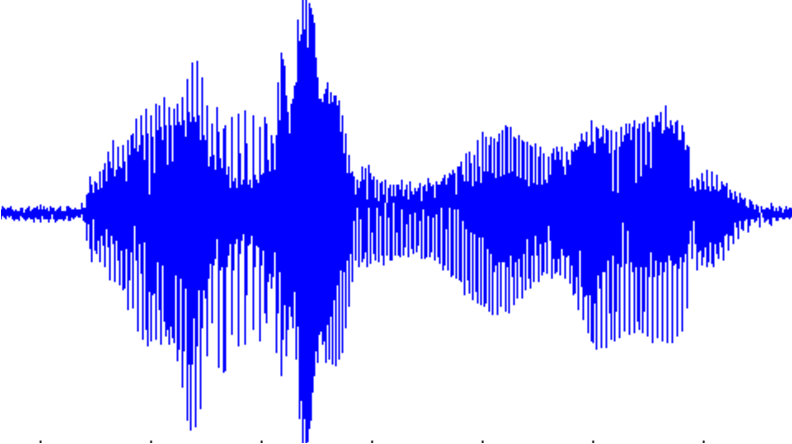
\includegraphics[width=1.2in]{figures/waveform.pdf}
\captionsetup{font=footnotesize}
 \captionof{figure}{Audio represented in waveform. }
\label{fig:waveform}
}
%
\item[Audio:] Audio is a rich source of information that can convey not only speech but any other sound that may not have an accurate textual description, for example, the sound of a heartbeat or the sound of waves. It is an effective media for evoking emotion or reflecting mood.\\
However, most audio lack appropriate visual representation, which makes it difficult to navigate or edit. Waveform is the most generic representation used in many applications, but it is ambiguous and hard to manipulate (Figure~\ref{fig:waveform}). 
For instance, detecting or separating the sound of one instrument from a music recording is a challenging research problem.\\

\item[Image:] A picture is worth a thousand words. Human perception is visually oriented, so images can be a powerful tool to communicate rich information intuitively in a small amount of space. Images are especially useful for conveying spatial relationships, structure, or detailed shape. Consider describing the layout of a building or the features of a face only using words versus showing a picture of the floor plan or the face.\\ 
On the other hand, it is difficult to convey information about movement or sequence using a still image. Oftentimes, text, labels or animation effects are attached to a still image to focus the viewers' attention to a specific part of the image or to clarify the intended message.\\

\item[Animation/Video:] Animations are created from a set of static frames whereas videos record a continuous event which is broken up into a series of frames. Both media are especially useful for illustrating concepts that involve motion or sequence.\\
As with audio, it takes time to navigate through the content of an animation or video and it is difficult to skim or search.\\

\item[Time:] In addition to having multiple modalities, audiovisual media is also intricately linked with time. Time imposes a linear structure to the media and is expressed, for example, with timelines on videos, scrollbars on websites and page numbers on slides. Whereas time provides a natural order to the media, it can also make non-linear interactions more cumbersome. For instance, watching a video from beginning to end is easy, but searching for specific scenes is harder.\\
Time also imposes a certain speed or pace to the media, and makes each \textit{moment}  within the media transient. Video frames, parts of webpages or slides are displayed for a limited amount of time and replaced with different, successive information. The abundance of concurrent and transitory information makes audiovisual media difficult to digest and manipulate compared to static media.\\
Finally, synchronization between multiple modalities is an essential part of audiovisual media. Effective navigation and manipulation of the media both require that the concurrence between multiple modes is appreciated and maintained. For instance, editing the audio track of a video normally requires editing the corresponding visual footage as well.
\end{description}

In sum, the complex interplay of multimodal information with each other and with time makes audiovisual media difficult to author, edit or navigate efficiently. Workflows around audiovisual media usually involve nonlinear navigation and iteration between different modalities. Unfortunately, conventional media browsers are best suited for linear navigation. Prevalent editing tools also handle each modality independently, leaving users to manage their interconnection manually. Both consumers and producers of audiovisual media have a right to be frustrated at the inefficiency caused by the lack of \emph{user-friendly} and \emph{media-friendly} interfaces that takes into account the users' workflows and characteristics of the media.\\ 
%
\section{The Goal: Effective Interfaces for Multimedia}
Just as effective multimedia carefully blends different types of media to advance the narrative, effective \textit{interfaces} for multimedia must capitalize the characteristics of each medium to expose the media to the users and provide tools to interact with it efficiently. Well-designed interfaces facilitate the users' workflow, be it authoring, editing or browsing, and whether it is linear or nonlinear. With the help of such interfaces, working with audiovisual media should be as simple and natural as working with text documents.\\

As natural as it seems today, text documents did not start out as an easy medium. Consider the 16-feet long scroll containing the text of the Diamond Sutra printed in 9th century China, or the Tripitaka Koreana, a collection of Buddhist scriptures carved onto 81,258 wooden printing blocks in 13th century Korea (Figure~\ref{fig:tripitaka}). 
%
\marginpar{
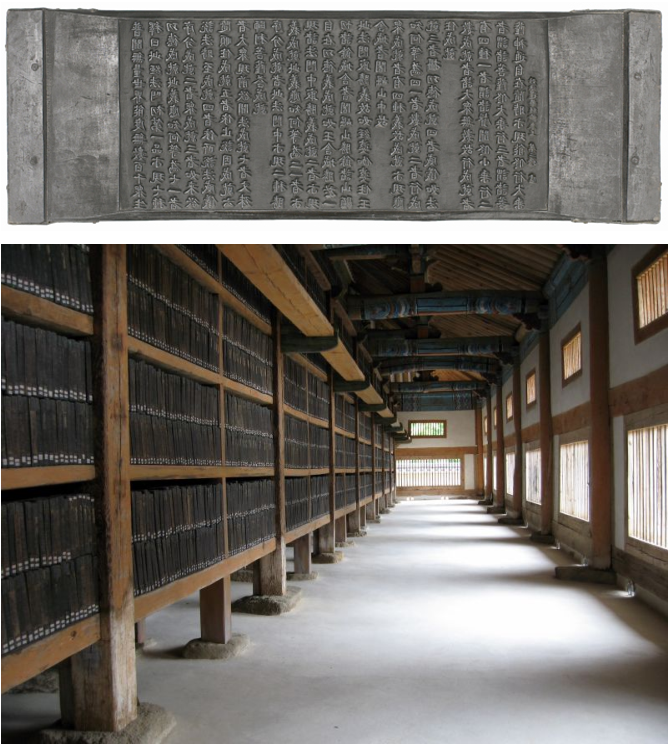
\includegraphics[width=1.2in]{figures/tripitaka_koreana.pdf}
\captionsetup{font=footnotesize}
 \captionof{figure}{Before convenient interfaces were developed, text documents were neither easy to author nor simple to navigate. Tripitaka Koreana, a collection of Buddhist scriptures cared onto 81,258 wooden printing blocks in 13th century Korea. (Above) Each wood block measures 24cm x 70cm. (Below) The blocks are stored in Haeinsa, a Buddhist temple in South Korea.}
\label{fig:tripitaka}
}
%
These text documents were neither painless to author nor easy to navigate. Even after the advent of digital word processors in the 1960s, it took several decades until the \emph{what-you-see-is-what-you-get} (WYSIWYG) form of word processors as we know them today became commonplace. Now, with online applications such as Google Docs, users can even collaborate on a single text document synchronously or asynchronously with ease. Wikipedia is an example of a new type of collaborative document that became possible through the development of online, collaborative text editors. \\

Similar to text documents, better interfaces can make it easier for users to author, edit, navigate and collaborate on audiovisual media. Improved efficiency can also lead to greater expressivity and even new types of audiovisual media. This dissertation takes a step towards this goal by exploring several approaches to designing effective interfaces for audiovisual media.

\section{Opportunities for Multimedia Interfaces}
Previously, we demonstrated that the complex combination of multiple modalities make multimedia especially difficult to navigate and manipulate. Yet, the same multimodal quality can be turned into opportunities for designing effective user interfaces for multimedia. The specific design strategy of an interface depends on the media as well as the interaction that the interface is trying to support (e.g., authoring, editing or browsing). Here, we outline several broad principles that emerged through our work on several different applications.\\
%
\begin{mldescription}
\mlitem{Harness spatial and temporal structure:} The different components of multimedia are tightly associated with each other in time and space. For instance, video frames that are adjacent in time are likely to have similar content. Simultaneous audio and visuals are also closely related to each other. Even within a single image or a slide, spatial layout can reveal meaningful patterns about the content.\\
Inferring the spatial and temporal structure embedded in the media can help design effective interactions. For one, explicitly visualizing the structure can help viewers navigate the media efficiently. In addition, interfaces can facilitate editing by keeping track of and maintaining meaningful structure, for instance, the synchronization between different components. \\
% 
\mlitem{Exploit different modalities to facilitate various types of interaction:} Each modality that compose audiovisual media lends itself more naturally to different types of user interaction or user tasks. For example, during navigation, text is easier to skim or search, whereas audio is better for listening to tonal nuances or flow. During authoring, speaking is faster than writing, but editing audio is generally more time consuming than editing text.\\
Interfaces for audiovisual media can take advantage of different modalities or representations to facilitate different parts of user tasks. For example, in Chapter~\ref{ch:voicescript}, we propose an interface for authoring voice recordings, which supports both authoring via speech and editing via text.  A key challenge in designing such multimodal interfaces is to enable seamless interaction between the different modalities. That is, edits in one modality should be translatable into meaningful operations in other modalities as well.  

\mlitem{Support direct manipulation with automation:} Hybrid approaches that combine direct manipulation with automatic algorithms have been proposed and successfully implemented in many application domains, including authoring of 3D models \cite{gal2009iwires, prevost2013make}, animations \cite{bai2016artist}, and illustrations \cite{chi2012mixt}. Automatic algorithms can greatly simplify tedious tasks and allow users to focus on the creative part of the workflow.\\
In light of the previous two principles, automatic algorithms can also take advantage of the inherent structure of the media or characteristics of different modalities. For example, in Chapter~\ref{ch:visualtranscript}, we use an automatic algorithm to extract  a set of static images from a video by analyzing the spatial and temporal structure of the visuals drawn continuously in the video. In Chapter~\ref{ch:voicescript}, we take advantage of text, which is a discrete modality that is easier to process automatically, in order to compare and align audio. Finally, in Chapter~\ref{ch:aparecium}, we use pre-authored digital slides to achieve, among other things, real-time beautification effects of hand-drawn strokes.\\ 
\end{mldescription}

As the following chapters will illustrate, these principles are instantiated for each application through a combination of interface design, visualization, algorithms and data structures.

%----------------------------------------------------------------------------------------
\section{Overview}
This dissertation is about designing effective interfaces to support the authoring and navigation of multimedia. We explore a range of applications -- navigating lecture videos, authoring speech recordings and delivering slide presentations. We originally considered these applications in separate publications, presented to different communities in computer graphics and human computer interaction. The goal of this text is to distill the common theme across these applications and present them in a unified way, along with insights gained over the course of our work.\\

Subsequent chapters are organized by application domain:
\begin{mldescription}
\mlitem{Navigating Lecture Videos (Chapter ~\ref{ch:visualtranscript}):}
Lecture videos are widely used for learning, but existing
video player interfaces are poorly equipped to support frequent learner tasks. It's difficult to search or skim the content, or view the lecture material at one's own pace. For these and other reasons, some people prefer to read lecture notes than to watch videos.\\
To facilitate learning with videos, we propose \emph{VisualTranscript}, a readable and skimmable interface for lecture videos. VisualTranscript transforms blackboard-style lecture videos into interactive lecture notes, interleaving static figures with hierarchically organized paragraphs of text.\\
We describe automatic algorithms to (1) extract a discrete set of key illustrations from the video frames, and (2) to analyze the audio content and classify sentences into two categorizes: depictive sentences that verbalize what the illustrations depict, and explanatory sentences that provide additional information not directly represented by the illustrations. Both algorithms take advantage of spatial and temporal structures inferred from the video.\\
We compared VisualTranscript with a standard video player, and a state-of-the-art interface designed specifically for blackboard-style lecture videos. User evaluation suggests
that users prefer VisualTranscript for learning and that VisualTranscript is
effective in helping them browse or search through lecture videos.
%
\mlitem{Authoring Speech Recordings (Chapter~\ref{ch:voicescript}):}
Speech recordings are central to modern media from podcasts
to audio books to e-lectures and voice-overs. Authoring these
recordings involves an iterative back and forth process between
script writing/editing and audio recording/editing. Unfortunately, most
existing tools treat the script and the audio separately, making
the back and forth workflow very tedious.\\
We present \emph{VoiceScript}, an interface to support a dynamic workflow for script
writing, audio recording and audio editing. VoiceScript integrates the
script with the audio such that, as the user writes the script or
records speech, edits to the script are translated to the audio
and vice versa.\\
Through informal user studies, we demonstrate that VoiceScript greatly facilitates the audio authoring process in various scenarios.
%
\mlitem{Delivering Slide Presentations(Chapter~\ref{ch:aparecium}):}
Presentations are an important component of both classroom
and online instruction, and presentation tools have a significant impact on how we teach and learn. Electronic slides, the dominant type of presentation technology today, has several shortcomings. Pre-authored slides take long time to prepare and restrict how contents are presented. There is little flexibility on the order and granularity of how information is displayed during the presentation.\\
We introduce \emph{Aparecium}, a presentation interface that helps presenters deliver flexible and engaging presentations by combining
the aesthetics and organization of electronic slides with
the spontaneity of inking. In Aparecium, presenters use inking
interactions to deliver slide presentations. With inking, presenters
can (1) reveal pre-authored content to the audience,
(2) make annotations on top of the slide, and (3) adjust the
slide layout to create blank space. Pre-authored slides help improve
the visual aesthetics and organization of the slides, while
inking enables presenters to have flexibility and fine-grained
control over the content and pace of the presentation.\\
In a user study comparing Aparecium with baseline presentation
tools, we found that our interface generally improves presentation
quality without increasing the burden on the presenter
at authoring or presentation time. Especially for text-centered
or process-driven content, both audiences and presenters preferred
presentations delivered using Aparecium.

\end{mldescription}
Finally, Chapter~\ref{ch:conclusion} reviews our contributions and discusses insights gained from our work. \\
The remainder of this chapter offers a brief overview of related work on multimedia interfaces.  
%----------------------------------------------------------------------------------------

\section{Related Work}
Not surprisingly, \emph{interfaces for multimedia} is a very broad subject that touches many fields of research, including human-computer interaction, computer vision, computer graphics, and even cognitive psychology. Instead of attempting to compile a comprehensive summary of the subject, we broadly categorize previous research according to different phases of users' workflows--browsing, authoring and delivery--and briefly review work that is directly related to the applications we present in this dissertation. 

\subsection{Browsing}
A main purpose of media browsing interfaces is to improve the users' efficiency by making it easier to find and absorb useful information--in short, to reduce the browsing time. Although specific techniques vary by media type and content, there are several common strategies that apply across different media. 
\begin{mldescription}
\mlitem{Displaying Compact Visual Representation:} Skimming and browsing are inherently visual tasks, and we perform them instinctively, for example, while we read or window-shop. A compact visual representation of the media can facilitate navigation by taking advantage of our natural visual capacity. \\
In case of videos, the final representation can be a shorter video ~\cite{he1999auto,ekin2003automatic,ngo2005video,lu2013story} or a set of still images~\cite{uchihashi1999video,barnes2010video,hwang2006cinema,boreczky2000interactive} extracted from the original video. It can also combine key frames with text from transcript~\cite{christel2002collages,pickering2003anses}. Static representations spatial structuring. For instance, . Enhanced by interactivity. \\
In case of audio, text for speech. Other visual representation. 
\mlitem{Analyzing Structure:}
\end{mldescription}


\subsection{Authoring}
Authoring covers a wide range of tasks from capturing, . 

\subsection{Delivery}


 

 % Chapter 1
%\cleardoublepage % Empty page before the start of the next part

%------------------------------------------------

%\ctparttext{You can put some informational part preamble text here. Illo principalmente su nos. Non message \emph{occidental} angloromanic da. Debitas effortio simplificate sia se, auxiliar summarios da que, se avantiate publicationes via. Pan in terra summarios, capital interlingua se que. Al via multo esser specimen, campo responder que da. Le usate medical addresses pro, europa origine sanctificate nos se.} % Text on the Part 2 page describing the content in Part 2

%\part{The Showcase} % Second part of the thesis

% Chapter 2
\newcommand{\systemname}[0]{VisualTranscript}
\chapter{Navigating Lecture Videos} % Chapter title
\label{ch:visualtranscript} % For referencing the chapter elsewhere, use
%
\begin{flushright}{\slshape    
The day is coming when the work done\\
by correspondence will be greater in amount\\
than that done in the classroom of our\\
academies and colleges.} \\ \medskip
--- \defcitealias{harper:1886}{William Rainey Harper}\citetalias{harper:1886} \citep{harper:1886}
\end{flushright}
%----------------------------------------------------------------------------------------
How viewers watch videos depends on the content of the video and the viewers'
needs. For example, watching a film in a theater is a very different experience
from watching a video tutorial on YouTube about how to cook brussel sprouts.
Even for a same video, someone who is watching it for the first time may have a
different approach from someone who has seen the video previously and is
watching it again only to review. In this chapter, we focus on the scenario of
watching lecture videos. \\

Lecture videos are growing in popularity, especially through Massive Open Online Courses
(MOOCs) and flipped classroom models.
However, learning with these videos using existing video player interfaces can
be challenging. Viewers cannot digest the lecture material at their
own pace, and it is also difficult to search or skim the content. For these and other
reasons, some viewers prefer lecture notes or textbooks to videos.\\

This chapter introduces \textbf{\systemname}, a readable
interface for lecture videos, that was designed to address some of these limitations. \systemname\ resembles lecture notes combining figures and text. To generate \systemname s, we take advantage of the spatial and temporal structures embedded in lecture videos. First, we segment the visual content
of a lecture into a set of discrete illustrations that correspond to equations, figures, or lines of text. Then, we analyze
the temporal correspondence between the transcript and the visuals to determine their relationships. Finally, based on the inferred relationships, we arrange the text and figures into a hierarchical and linear layout. \\

We compare \systemname\ with a standard video player, and a state-of-the-art interface designed specifically for 
lecture videos. User evaluation suggests that users prefer \systemname\ for the task of learning and that \systemname\
facilitates browsing and searching in lecture videos.

%----------------------------------------------------------------------------------------

\section{Introduction}
Despite the increasingly important and broad role of lecture videos in education, learning from such videos poses some challenges. 
%
It is difficult for viewers to consume video content at their own pace~\cite{chi2012mixt}.
%
To skip quickly through familiar concepts or slowly review more difficult material, the viewer must interrupt playback and scrub back-and-forth in the timeline.
%
It is also difficult to find specific information in a video. While scrubbing allows users to browse the visual information in the lecture, it is not effective for skimming the audio content, which often includes critical explanations and context that accompany the visuals. As an alternative, some platforms (e.g., Khan Academy and YouTube) provide synchronized transcripts that allow users to click on a phrase and play the video at that location. However, skimming the transcript for relevant content can also be challenging since the text is not structured, and viewers must click on various parts of the text to see the corresponding visuals. 
%
Finally, it is hard to get a quick overview of the lecture content without watching the entire video. 
For these and other reasons, some people prefer static learning materials such as textbooks or printed lecture notes over videos.\\

Inspired by lecture notes, we present \systemname, a readable interface for both the visual and audio content of a lecture video that facilitates reviewing, browsing and navigation. 
%
We focus on blackboard-style lectures that show a possibly infinite blackboard where the instructor writes down by hand the content of the lecture. \systemname s aggregate the full lecture content in a structured format where visual information is segmented and grouped with the corresponding narration text. For example, Figure~\ref{Fig:videonote_example} shows our automatically generated output for math lectures that interleaves verbal explanations with corresponding equations written on the board. 
%
By default, \systemname s hide redundant information to show a compact representation of the content that viewers can expand interactively to show relevant details (Figure~\ref{Fig:videonote_expanded}). 
%
Presenting video content in this manner allows users to review the lecture at their own pace while getting both the visual and textual information in a readable, skimmable format.
%
\systemname s is also linked to the video such that clicking on the text or the visuals plays the video from the corresponding location.
%
In this respect, \systemname s offer many of the benefits of traditional static media, such as textbooks and lecture notes, while also giving viewers direct access to the video content.\\

There are two main challenges in transforming a video and its transcribed audio into a \systemname : (1) visuals, which are drawn progressively on the board, must be discretized into  a set of meaningful figures, and (2) such figures and text representing the audio content must be organized into a compact, structured format that emphasizes the relationships between the two channels of information.
%
To segment the visuals into meaningful figures, we propose a dynamic programming approach that takes into account both the spatial layout of strokes and the time when they were drawn. We further time-align the transcript with the audio and use this alignment to establish correspondences between the visuals and the text. Finally, we use the visual-text correspondence to detect redundant information and arrange the content in a compact, sequential layout where the text is organized into readable paragraphs.\\

We evaluate our approach with a user study that compares \systemname\ with a standard video player with an interactive transcript, and an existing state-of-the-art visual-based video player developed by Monserrat et al \cite{monserrat2013notevideo}. We measure performance on summarization and search tasks, and observe how the participants interact with the interfaces. Evaluation results suggest that \systemname\ is indeed an effective interface for studying lecture videos. Specifically, users performed best using \systemname\ for search tasks involving text. Users noted that \systemname\ helped them to get a quick overview of the video including the details conveyed only through the text, and to efficiently focus on parts of interest. They also found the structured text easier to read and connect to relevant visuals than the baseline text-only transcript. In a post-study survey, users strongly preferred our interface for learning over the other two interfaces.\\

%----------------------------------------------------------------------------------------
\section{Previous Work}
%
\subsection{Video Visualization}
There is a large body of work that aims to automatically summarize videos to facilitate navigation and browsing, but most research focuses on live action footage which is very different from educational videos.  Recent survey papers \cite{truong2007video,borgo2011survey} comprehensively review these techniques, which can be broadly divided into two classes according to their output: \textbf{video skims} and \textbf{still-image abstracts}. \\

Video skims \cite{he1999auto,ekin2003automatic,ngo2005video,lu2013story} summarize a longer video with a shorter video, usually consisting of segments extracted from the original video. These skims retain audio and motion elements and are especially useful for understanding dynamic scenes, but they are less suitable for conveying the dense, static information of blackboard-style lectures. \\

Still-image based methods~\cite{uchihashi1999video,barnes2010video,hwang2006cinema,boreczky2000interactive}
primarily focus on conveying the visual content of a
video in static form through a collection of salient images extracted from the video.~\cite{christel2002collages} and~\cite{pickering2003anses} developed a still-image based method specific to news stories that combines text and images into summaries.\\

Most relevant to our work is~\cite{choudary2007summarization}, which summarizes blackboard-style lectures by creating a panoramic frame of the board. In addition to the visual content presented on the board, our interface includes the audio content and therefore maintains the sequence of the lecture and makes textual content also directly accessible.\\

\subsection{Tools for Online Lecture Videos}
Kim et al. use interaction data collected from MOOC platforms to introduce a set of techniques that augment existing video interface widgets~\cite{kim2014data}. For lecture videos based on slides, Li et al. use separate slides to automatically generate table-of-content overviews~\cite{kim2014data}. These works \textit{annotate} the original video with useful data to facilitate navigation, but do not reformat the video content. Pavel et al. provide a tool to create \textit{video digests}, structured summaries of informational videos organized into chapters and sections~\cite{pavel2014video} . They use  only the transcript to segment and summarize the video, whereas we leverage both the visual and audio content.\\

Most closely related to our work is Monserrat et al.'s interface \cite{monserrat2013notevideo}, which presents a summary image of blackboard-style lecture videos. Their image is composed of click-able visual links to support spatial and temporal navigation. Although they provide a search box for the transcript, text is not included as part of their summary display.

%----------------------------------------------------------------------------------------
\section{Design Principles}
\label{sec:principles}
%
The design of \systemname\ is informed by the following key characteristics of blackboard-style lectures:
%
\subsection*{Lectures present information progressively.}
\begin{figure}[h!]
    \centering
        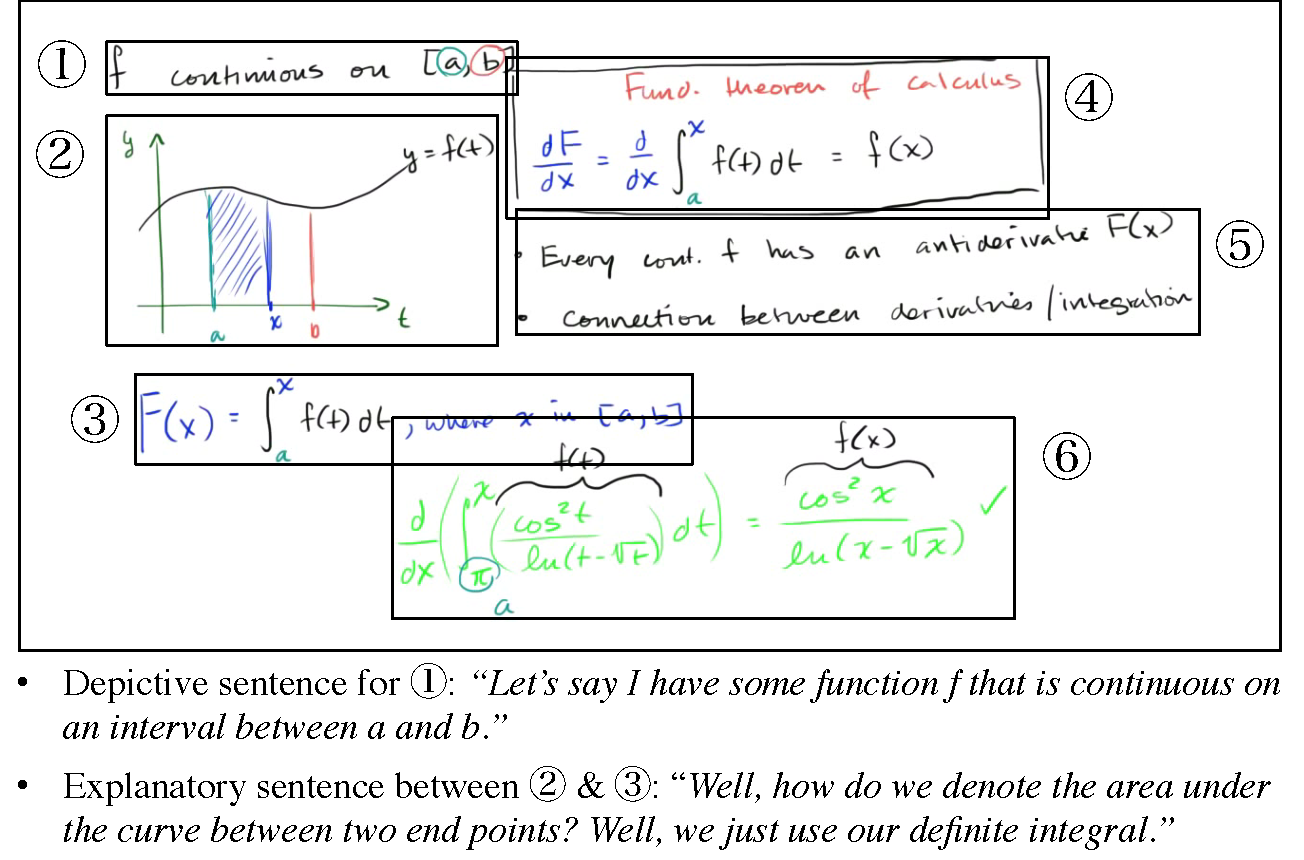
\includegraphics[width=\textwidth]{figures/keyideas.pdf}
    \caption{(top) Lectures convey concepts progressively. Here, the labels (1 through 6) show the order in which concepts were presented. They also organize visuals into discrete entities (outlined in this visualization with bounding boxes). (bottom) Verbal explanations during lectures are either depictive or explanatory.}
    \label{Fig:key_ideas}
\end{figure}
%
Most lectures convey concepts in a progressive manner where each new piece of information builds on the previously presented content.
For example, Figure~\ref{Fig:key_ideas} (\textit{top}) shows a panoramic image of the board for an entire lecture, where the labels show the order in which the contents were presented. Understanding the lecture often requires knowing this order.
%
To emphasize presentation order, our \systemname\ arranges all the content within the video in a top-to-bottom linear format.
%
\subsection*{Visuals are organized into discrete entities.} The visual content of a lecture is typically organized into well-defined entities (e.g., a line of text, an equation, an explanatory figure) that correspond to the set of presented concepts. 
%
For example, Figure~\ref{Fig:key_ideas} (\textit{top}) shows six visual entities in a calculus lecture.  Each visual entity consists of strokes that are close together in either space or time. Moreover, since people are accustomed to parsing visual information line-by-line, from top to bottom, and left to right, visual entities are often laid out in the same manner. 
%
Building on this observation, our system segments drawings on the board into visual entities based on their spatial alignment and temporal proximity.
%
\subsection*{Audio content complements visuals.}
In our analysis of lecture videos, we found that verbal explanations tend to serve one of two broad objectives. Explanations given while the instructor is \emph{not} drawing are often \emph{explanatory}, providing additional information not directly represented in the visuals or making connections between drawings. On the other hand, explanations given while the instructor is drawing are typically more \emph{depictive}, repeating or reading aloud the visual information (Figure~\ref{Fig:key_ideas}, \textit{bottom}).
%
While depictive explanations can help viewers follow along with the video, they often result in long, repetitive transcript text that is cumbersome to read or skim through. This problem is exacerbated by the fact that spoken explanations are usually colloquial.\\

Our interface automatically categorizes transcript text as either explanatory or depictive. In the default view, we hide depictive sentences and only show explanatory text interspersed with the set of visual entities extracted from the video. 
Large et al.~\cite{large1995multimedia} and Christel and Warmak~\cite{christel2001effect} have shown that such combinations of pictures and captions aid recall and comprehension as well as navigation of video material.
%
Our design gives the viewer relevant context for understanding the visual information without cluttering the output with redundant text. Users can click on a visual entity to see the corresponding depictive sentences.
\cleardoublepage
%----------------------------------------------------------------------------------------
\section{The \systemname\ Interface}
%---------------------------------------------------------------------------------------
\begin{figure}[h!]
    \centering
        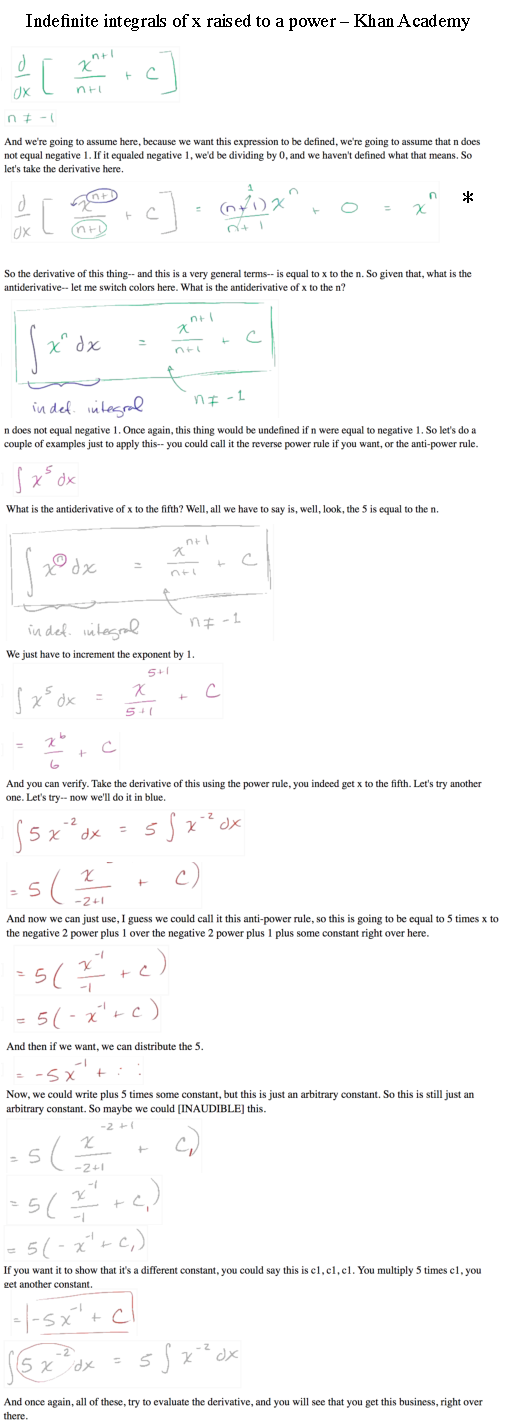
\includegraphics[width=\textwidth]{figures/videonote_example.pdf}
    \caption{Examples of two VisualTranscript outputs from Khan Academy Videos. (Top)\textit{'Indefinite integrals of x raised to a power'} and (Bottom)\textit{'Fundamental theorem of calculus}. Users can click on a figure to expand step-by-step details. For example, the equation marked by '*' is expanded in Figure~\ref{Fig:videonote_expanded}.}
    \label{Fig:videonote_example}
\end{figure}
%
%---------------------------------------------------------------------------------------
Based on these observations, we designed \textbf{\systemname}, a readable and printable interface that presents both the visual and audio content of a lecture video. Since \systemname\ contains all of the visual and audio information from the original video, it can be used by itself to study the content. Alternatively, it can be linked to the original lecture video to function as an interactive navigation aid. Similar to Monserrat et al's interface \cite{monserrat2013notevideo}, clicking on a visual entity or a transcript sentence plays the original video at that point in time. As the video is playing the corresponding visual entity and transcript sentence are highlighted. \\

Figure~\ref{Fig:videonote_example} shows two examples of \systemname\ created from Khan Academy videos. Please visit \url{https://people.csail.mit.edu/hishin/projects/visual_transcripts/abstract.html} for the interactive version of these examples. Given an input video and its transcript, we generate \systemname\ automatically using the algorithms described in the next section. To test the robustness of our method, we generated \systemname s of 20 lecture videos from 11 different instructors. Please view the appendix for all the results. Here we highlight some of the key features of \systemname .\\
%

\subsubsection{Linear format highlights lecture progression.} 
The layout of text and visual entities in \systemname\ often emphasizes the instructor's thought process and clarifies the intermediate steps that lead to a result. Figure~\ref{Fig:feature_highlight}~(left) compares equations in the final view of the blackboard at the end of the lecture with a \systemname\ output. 
%
\begin{figure}[h!]
    \centering
    \begin{subfigure}[t]{2.4in}
        \centering
        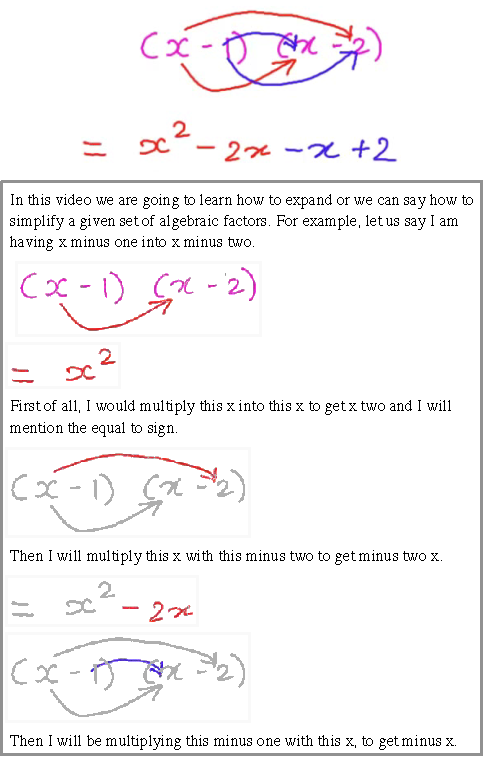
\includegraphics[width=0.8\textwidth]{figures/progression_ex.pdf}
    \end{subfigure}%
~
       \begin{subfigure}[t]{1.8in}
        \centering
        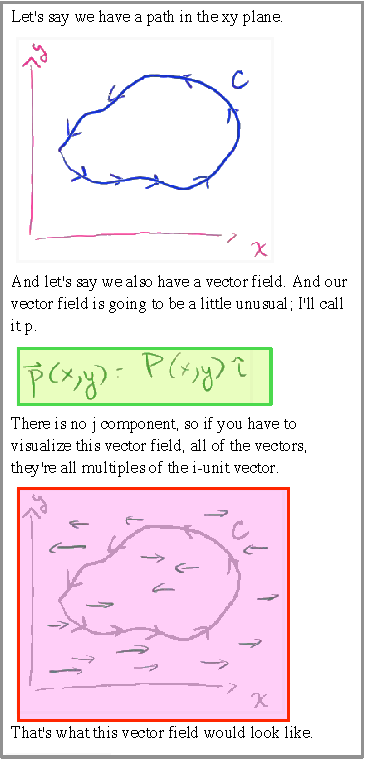
\includegraphics[width=0.8\textwidth]{figures/intersperse_highlight.pdf}
    \end{subfigure}
    \caption{(Left, bottom) \systemname\ shows the step-by-step progression of an equation  which is not apparent in the (left, top) final view of the board. (Right) Interspersing text with visuals clarifies the connection between the illustration of a vector field (pink hightlight) and its equation (green highlight). Compare with the leftmost example in Figure~\ref{Fig:visual_line_output}.}
    \label{Fig:feature_highlight}
\end{figure} 
%

Although both views show the same set of equations, in the blackboard view (top) it is difficult to infer how the equations relate to and build upon each other. In contrast, the \systemname\ output (bottom) shows a step-by-step progression of the visual content. 


\subsubsection{Interspersing text with visuals clarifies connections.} 
A purely visual summary of the video omits verbal explanations, whereas a purely textual summary (i.e., transcript) can be confusing without the corresponding visuals. Instead, \systemname\ interleaves explanatory text and visual entities. This makes it easy to see the connection between illustrations, or the context of an illustration. For instance, compare the leftmost example in Figure~\ref{Fig:visual_line_output}, which shows a final view of the blackboard and Figure \ref{Fig:feature_highlight}~(right), which shows the \systemname\ for the same video. In the former, it is difficult to see the connection between the illustration (pink highlight) and the equation to its right (green highlight) without listening to the lecture. In the latter, the text in-between explains clearly that the equation represents the vector field depicted in the illustration.

\subsubsection{Hierarchical organization show different levels of detail.} 
By default, \systemname\ hides redundant depictive text that just describes the corresponding visuals. Users can click on a visual entity to reveal the corresponding hidden text and read the details. In the case of a long equation or a complicated illustration, the expanded view breaks up the visual and textual information 
into easy-to-read blocks (Figure~\ref{Fig:videonote_expanded}). 
%
\begin{figure}[h!]
        \centering
        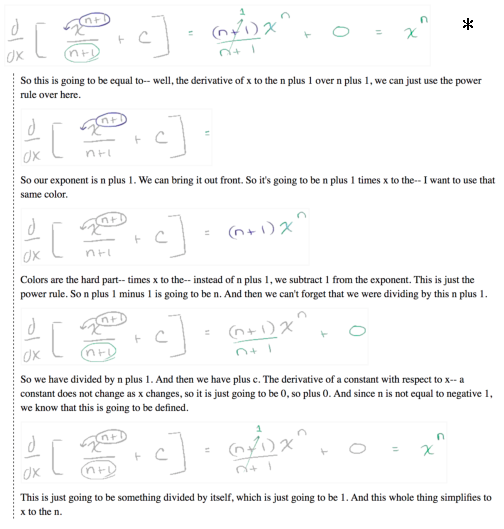
\includegraphics[width=0.7\textwidth]{figures/videonote_expand.pdf}
	\captionsetup{font=footnotesize}
        \caption{\systemname\ is organized hierarchically. The default view hides descriptive details to present a compact summary (Figure~\ref{Fig:videonote_example}*). Users can click on a higher-level figure to expand its detailed description and step-by-step derivation.} 
        \label{Fig:videonote_expanded}
\end{figure}\\
%
%----------------------------------------------------------------------------------------

\section{Algorithms}
There are three main steps to create \systemname . First, we
segment the visual content of a lecture into visual entities using a
dynamic programming approach (\ref{sec:segmentation}). Then, we 
structure the transcript content by computing temporal correspondences
between visual entities and transcript sentences
(\ref{sec:text_corr}). Finally, we generate a \systemname\ by interleaving visual entities with transcript text (\ref{sec:layout}). The rest of this section describes each of these steps in detail.
%
\subsection{Pre-processing}
The visual content in blackboard-style lectures consists of \emph{strokes},
the set of foreground pixels generated during one continuous drawing action.
In the context of a graphics tablet, a stroke corresponds to the continuous
path of a pen while maintaining contact with the writing surface. 
Since our input is a recorded video and we do not have the vector information of the strokes, instead we extract
individual strokes from the video frames using a method similar to
\cite{monserrat2013notevideo}.  We detect the start and end time of
each drawing action by comparing the number of foreground pixels in
consecutive frames. A large increase marks the start of an action,
while no change marks the end. The difference image between the end
and start frames gives an image of the stroke drawn during that
period.
The manual steps involved in this process are (1) identifying the cursor image, which is automatically removed from all frames, (2) setting a threshold for foreground/background separation, and (3)  setting a smoothing window to get rid of the noise in the foreground pixel count. Depending on the instructor's writing speed, a typical stroke
comprises several characters to several words, or it can also be a
part of an illustration or a graph (Figure~\ref{Fig:stroke_examples}).\\
%
\begin{figure}[h!]
    \centering
        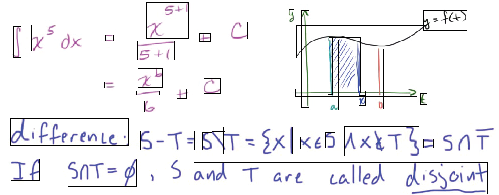
\includegraphics[width=0.8\textwidth]{figures/strokes.pdf}
    \caption{Examples of strokes (marked by black bounding boxes) extracted from video frames.} 
    \label{Fig:stroke_examples}
\end{figure}

In addition
to the visuals, lecture videos include an audio track with the instructor's
spoken explanations. Several on-line video lecture platforms (e.g. Khan Academy,
YouTube) provide transcripts of the audio. We assume such transcripts and
we use an online audio transcription service (\url{castingwords.com}) if they are
not available. 
%
\subsection{Segmenting Visual Content}
\label{sec:segmentation}
\marginpar{
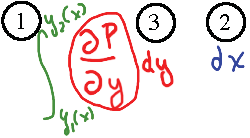
\includegraphics[width=1.2in]{figures/greedy_ex-2.pdf}
\captionsetup{font=footnotesize}
 \captionof{figure}{Without considering the semantics of these symbols and before the last stroke ($\frac{\delta p}{\delta y}dy$) is inserted, the first two strokes ($-\int^a_b$ and $dx$) appear like two separate equations with a large space between them.}
\label{fig:baselineinset}
}
One straightforward strategy for grouping strokes into visual entities
is to process strokes in the order they are drawn and decide whether
each stroke represents the start of a new visual entity or is part of
an existing visual entity formed by previous strokes \cite{mynatt1999flatland}.
While this simple, greedy approach works in some cases, there are many
scenarios where it leads to poor segmentations. For example, in
Figure~\ref{fig:baselineinset}, there is a large space between the first stroke ($-\int^a_b$, \raisebox{.5pt}{\textcircled{\raisebox{-.9pt} {1}}}) and the second stroke ($dx$, \raisebox{.5pt}{\textcircled{\raisebox{-.9pt} {2}}}). Without considering the semantics of these symbols, 
they appear to be separate equations. However, once we consider 
the subsequent set of red strokes(\raisebox{.0pt}{\textcircled{\raisebox{.2pt} {3}}})
 it becomes clear that this is not the best segmentation. In general, computing good stroke segmentations requires considering
the global configuration of strokes in both space and time. \\

In this respect, the problem of segmenting strokes into visual
entities is analogous to the
\emph{line-breaking} problem, i.e., arranging the words of a paragraph
into lines.  In both cases, we want to segment a sequence of elements
(strokes or words) into an optimal set of groups (visual entities or
lines) defined by some scoring function over candidate entities or lines.
An important difference is that in the traditional line-breaking problem, only a
contiguous set of words can be put on the same line. In our case,
strokes in one visual entity can be interspersed by strokes in a
different visual entity. For example, the instructor may
go back and forth between two lines of equations, or
between a graph and an equation (Figure~\ref{Fig:line_order}).\\
%
\begin{figure}[h]
        \centering
        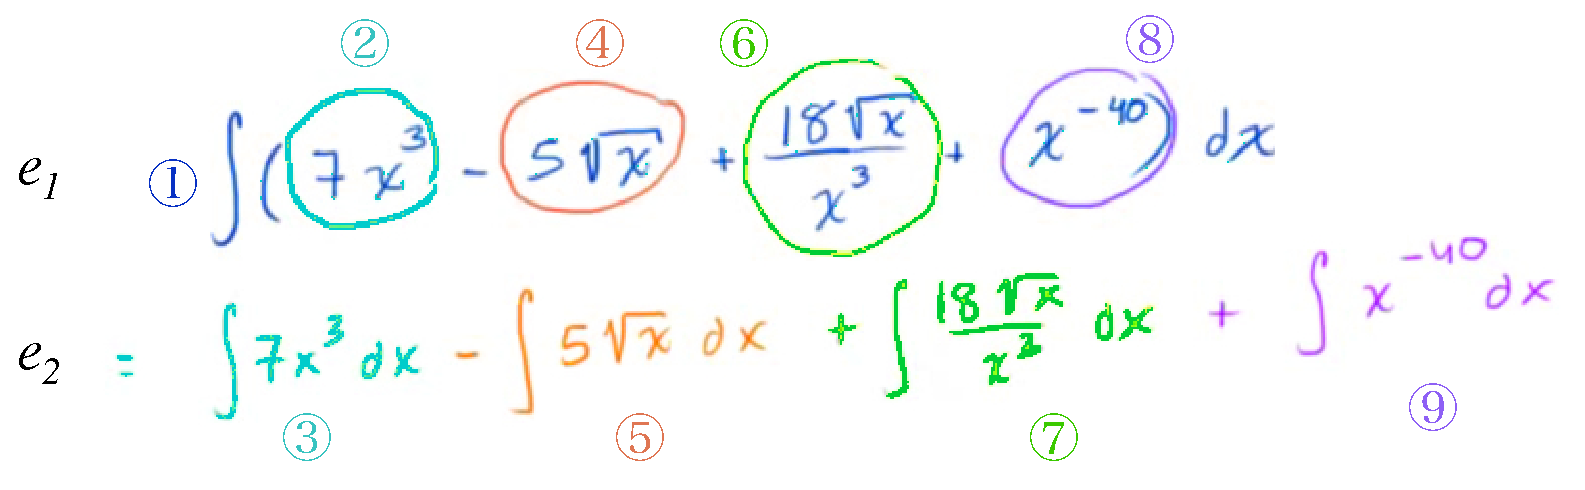
\includegraphics[width=0.8\textwidth]{figures/line_order.pdf}
        \caption{The instructor goes back and forth between writing two lines,
$e_1$ and $e_2$. The order of strokes 1-9 is as indicated.}
        \label{Fig:line_order}
\end{figure}\\
%

Given these observations, we propose a dynamic programming approach for
stroke segmentation based on the classic optimal line-breaking
algorithm~\cite{knuth1981breaking} that handles non-contiguous grouping.
We first explain the high-level structure of the algorithm before
describing the scoring function in detail.
%
\subsubsection{Algorithm Overview}
Figure \ref{Fig:pseudocode} gives a detailed pseudo-code of our segmentation algorithm.\\    
%
\begin{figure}[h!]
        \centering
        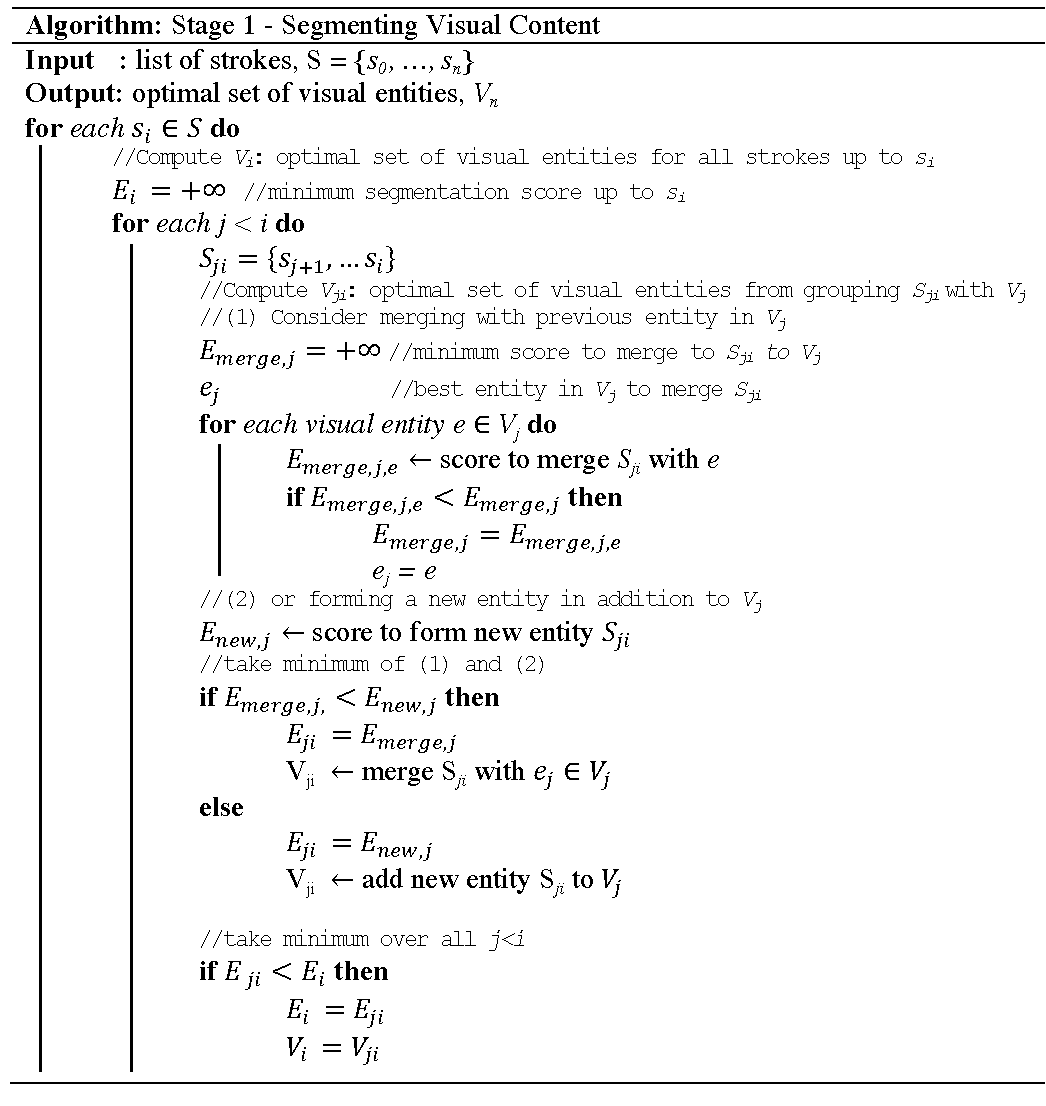
\includegraphics[width=\textwidth]{figures/pseudocode_image.pdf}
	\captionsetup{font=footnotesize}
        \caption{We use dynamic programming to segment strokes into an optimal
set of visual entities. For each stroke, $s_i$, the algorithm considers all previous
partial solutions, $V_{j<i}$ and $S_{ji}=\{s_{j+1}, ..., s_i\}$. For each
$V_j$, it considers two possibilities: merging $S_{ji}$ with an existing
entity or forming a new entity.}
        \label{Fig:pseudocode}
\end{figure}\\
%
Given a sequence of $n$ strokes $S = \{s_o,\dots,s_{n-1}\}$ ordered by
when they appear in the video, we find the optimal set of inter-stroke
boundaries that segment the strokes into visual entities. We refer to the boundary between $s_i$ and $s_{i+1}$ as
$b_i$.
%
Our algorithm processes the strokes in order and for each $s_i$
computes and records the optimal set of visual entities $V_i$ formed
by all strokes up to $b_i$, along with the total score $E(V_i)$ of
this partial solution.
%
To determine the optimal partial solution for stroke $s_i$, we
consider each previous boundary $b_j$ where
$\setlength{\thickmuskip}{0mu} j<i$, and evaluate two possible ways of
grouping the set of strokes $S_{ji} = \{s_\text{j+1},
\dots,s_\text{i}\}$: 1) merging $S_{ji}$ with one of the existing entities
in $V_j$, or 2) forming a new entity with $S_{ji}$. 
%
Allowing $S_{ji}$ to be merged with existing entities enables our
algorithm to support non-contiguous stroke groupings.
%
We take the better (lower) of the two scores for $S_{ji}$ and add it
to $E(V_j)$ to obtain the total score for the proposed
segmentation. After considering all candidate boundaries $b_j$, we
identify the partial solution with the minimum segmentation score and
record the corresponding set of entities as $V_i$ and the score as $E(V_i)$.
%
Once the algorithm iterates through all strokes, $V_n$ gives the
optimal set of visual entities for the entire lecture.
%
%
\subsubsection{Scoring Function}
The dynamic programming algorithm described above requires a scoring
function that evaluates the goodness of candidate visual entities
formed by sets of strokes. We define this scoring function based on
several observations: Strokes within a visual entity are (1) compactly arranged and (2) horizontally aligned. In addition, (3) separate visual entities are spatio-temporally distant from each other.
%
\paragraph{(1) Visual entities are compact.} Strokes that belong together
in the same visual entity are typically arranged in a compact way. We
consider two measures of compactness for a visual line:
horizontal and vertical.

\begin{figure}[h!]
	\centering
        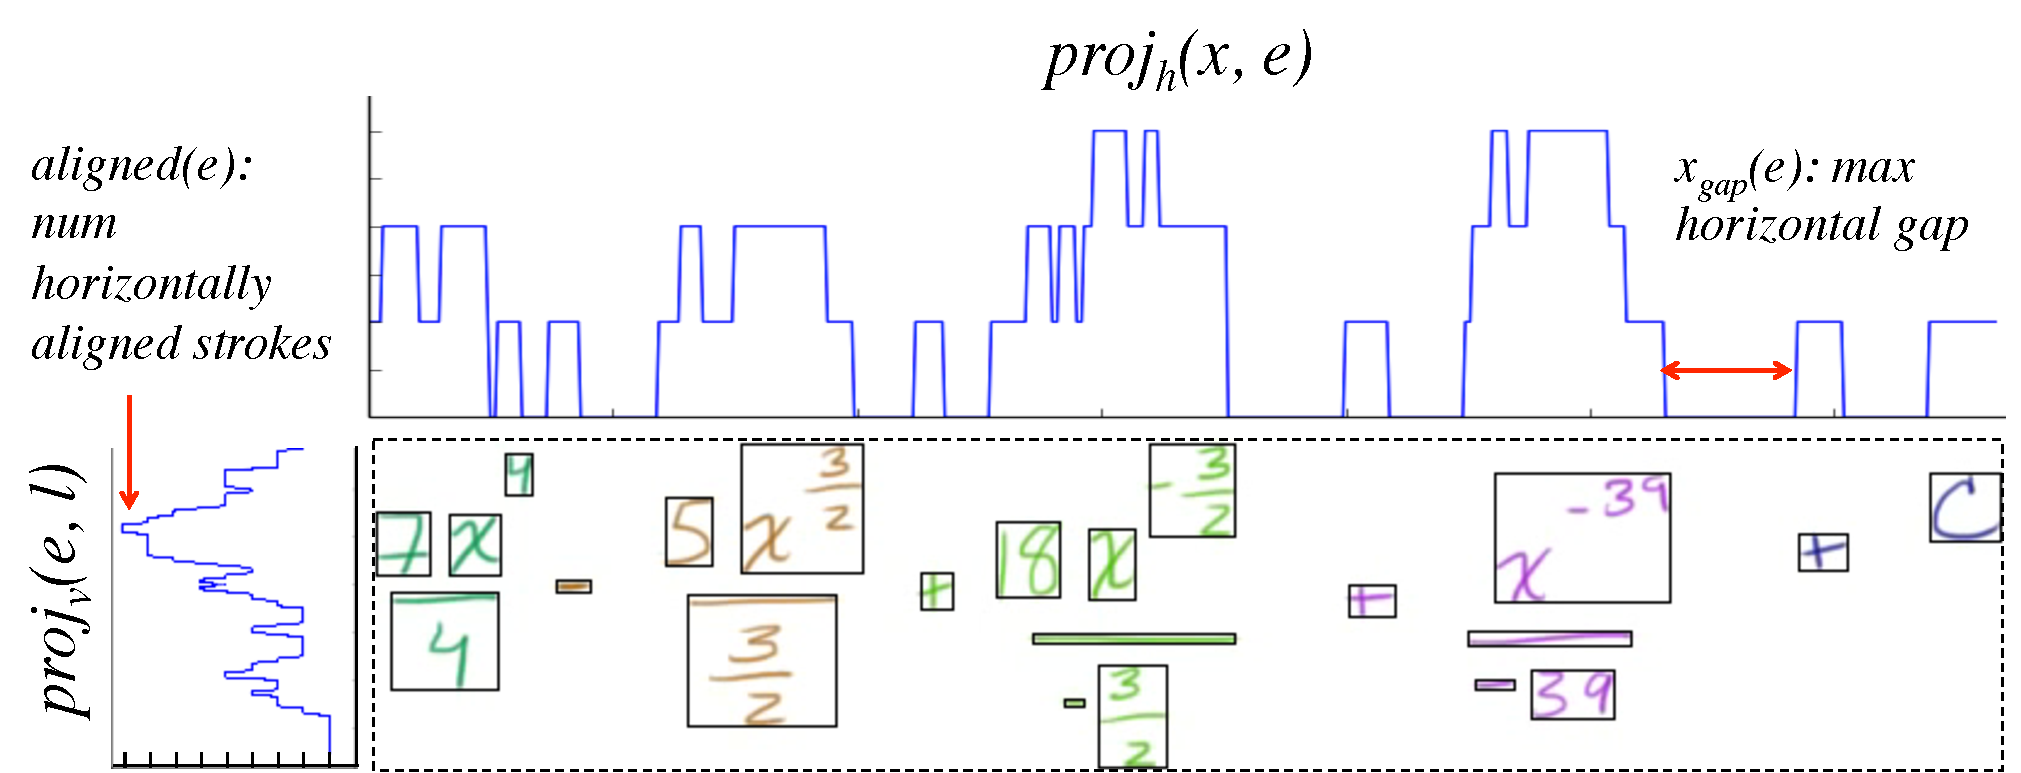
\includegraphics[width=0.8\textwidth]{figures/projection_function.pdf}
        	\captionsetup{font=footnotesize}
        \caption{Horizontal ($proj_h$) and vertical ($proj_v$) projection functions of strokes in a line. In this example, $y_\text{gap}(e)=0$.}
        \label{Fig:projection_function}
\end{figure}

\begin{itemize}
\item \textbf{Horizontal Compactness:} Intuitively, horizontal compactness is related to the horizontal
\emph{gap} between strokes within a visual entity. Figure \ref{Fig:projection_function}
shows an illustration of how gaps between strokes are measured. First, we define a horizontal projection function for a set of strokes, $S$, as 
\begin{equation}
proj_h(x, S) = \big{|}\{s\in S \small{|} x_\text{min}(s)\le x \le x_\text{max}(s)\}\big{|}
\label{Eq:projh}
\end{equation}\\  
where $x_\text{min}(s)$, and $x_\text{max}(s)$ are the minimum and maximum $x$-coordinates of the bounding box of stroke $s$ respectively. Then, the maximum horizontal gap of a visual entity $e$ is
 \begin{equation}
 x_\text{gap}(e) = \argmax_{x_i, x_\text{i+1}} (x_\text{i+1}
 - x_i)
 \end{equation}
where $x_i$ and $x_\text{i+1}$ are distinct consecutive elements in the ordered set $X =\{\,x \mid proj_{h}(x,e)\ne 0\,\} $. We observed that the horizontal gap between different visual entities
is usually around 100 pixels or more, so we define a horizontal compactness
term $C_{h}$ that imposes harsher penalties when the maximum
horizontal gap exceeds this distance.
\begin{equation}
C_{h}(e) = \big(\frac{x_\text{gap}(e)}{100}\big)^2
\end{equation}

\item \textbf{Vertical Compactness:} Vertical compactness is defined similarly in terms of a vertical projection
function, $proj_{v}$, the maximum vertical gap,
$y_\text{gap}(e)$, and a typical vertical gap of 40 pixels between
different visual entities.
\begin{equation}
C_v(e) = \big(\frac{y_\text{gap}(e)}{40}\big)^2
\end{equation}
\end{itemize}

\paragraph{(2) Strokes within a visual entity are aligned horizontally.} With the exception
of certain illustrations such as graphs, the strokes in most visual
entities are horizontally aligned (e.g., equations, lines of
text). Thus, we prefer to group horizontally aligned strokes into a single
entity. The number of horizontally aligned strokes in each visual entity is computed by taking the mode of its vertical projection function (Figure \ref{Fig:projection_function}).
\begin{equation}
aligned(e) = \argmax_{y_\text{min}(e) \le y \le y_\text{max}(e)} proj_v(y)
\end{equation}
We then define an alignment term $C_a$ whose contribution gradually
diminishes with the total number of aligned strokes.
\begin{equation}
C_a(e) = aligned(e)-\frac{1}{aligned(e)+1}
\label{Eq:n_align}
\end{equation}

\paragraph{(3) Distinct visual entities are spatio-temporally distant from each other.} This observation
is complementary to the first observation, i.e., visual entities are
compact. Whereas strokes that belong together are written close
together, instructors usually leave some space on the board, for
example, between lines of equations or separate illustrations. We
express this property by penalizing any overlap between distinct
visual entities, measured by the overlapping
area between their bounding boxes. In particular, we define the overlap
penalty term
\begin{equation}
P_{o}(V) = \sum_{e_i,e_j \in V, i \neq j}\big(\frac{area(e_i\cap e_j)}{min(area(e_i), area(e_j))}\big)
\label{Eq:overlap_penalty}
\end{equation}
A similar property holds in the temporal domain. For example, after
writing a single line of an equation and before going on to the next
line, there is a brief pause while the instructor moves the cursor to
the next position or provides some verbal explanation. We compute the
temporal distance between two consecutive strokes across visual entity
boundaries.
\[
    t_\text{dist}(s_i, s_\text{i+1})= 
\begin{cases}
   0, \text{if } s_i, s_\text{i+1 } \text{belong to the same visual entity}\\
   start(s_\text{i+1}) - end(s_i), \text{otherwise}
\end{cases}
\]
where $start(\cdot)$ and $end(\cdot)$ are the start and end times of
when a stroke is drawn in the video. We penalize visual entity
boundaries with a small temporal gap.
\begin{equation}
P_{t}(V) = \sum_{i = 0}^{n-1}\frac{1}{t_\text{dist}(s_i, s_{i+1})}
\end{equation}
where $n$ is the total number of strokes.\\

\paragraph{Combining scoring terms.} So far, we have defined terms that measure the compactness ($C_h, C_v$) and horizontal alignment ($C_a$) of an individual visual entity $e$, as well as the spatio-temporal distance ($P_o, P_t$) between a set of candidate entities $V$. 
%
We combine all these terms into a single scoring function $F$ as follows.  
\begin{align}
F(V) = &\sum_{e \in V}[C_v(e) + 0.5C_h(e)- C_a(e)]&\\
&+ P_o(V) + P_t(V)
\end{align}\\
The factor of 0.5 puts a smaller weight on horizontal versus vertical
gaps. Higher values of $C_a$ indicate more horizontally aligned strokes and better segmentation, so we put a minus in front.\\

The final output of our algorithm is a grouping of all the strokes on the
board into a set of meaningful visual entities (Figure~\ref{Fig:visual_line_output}).
%
\begin{figure}[h!]
        \centering
        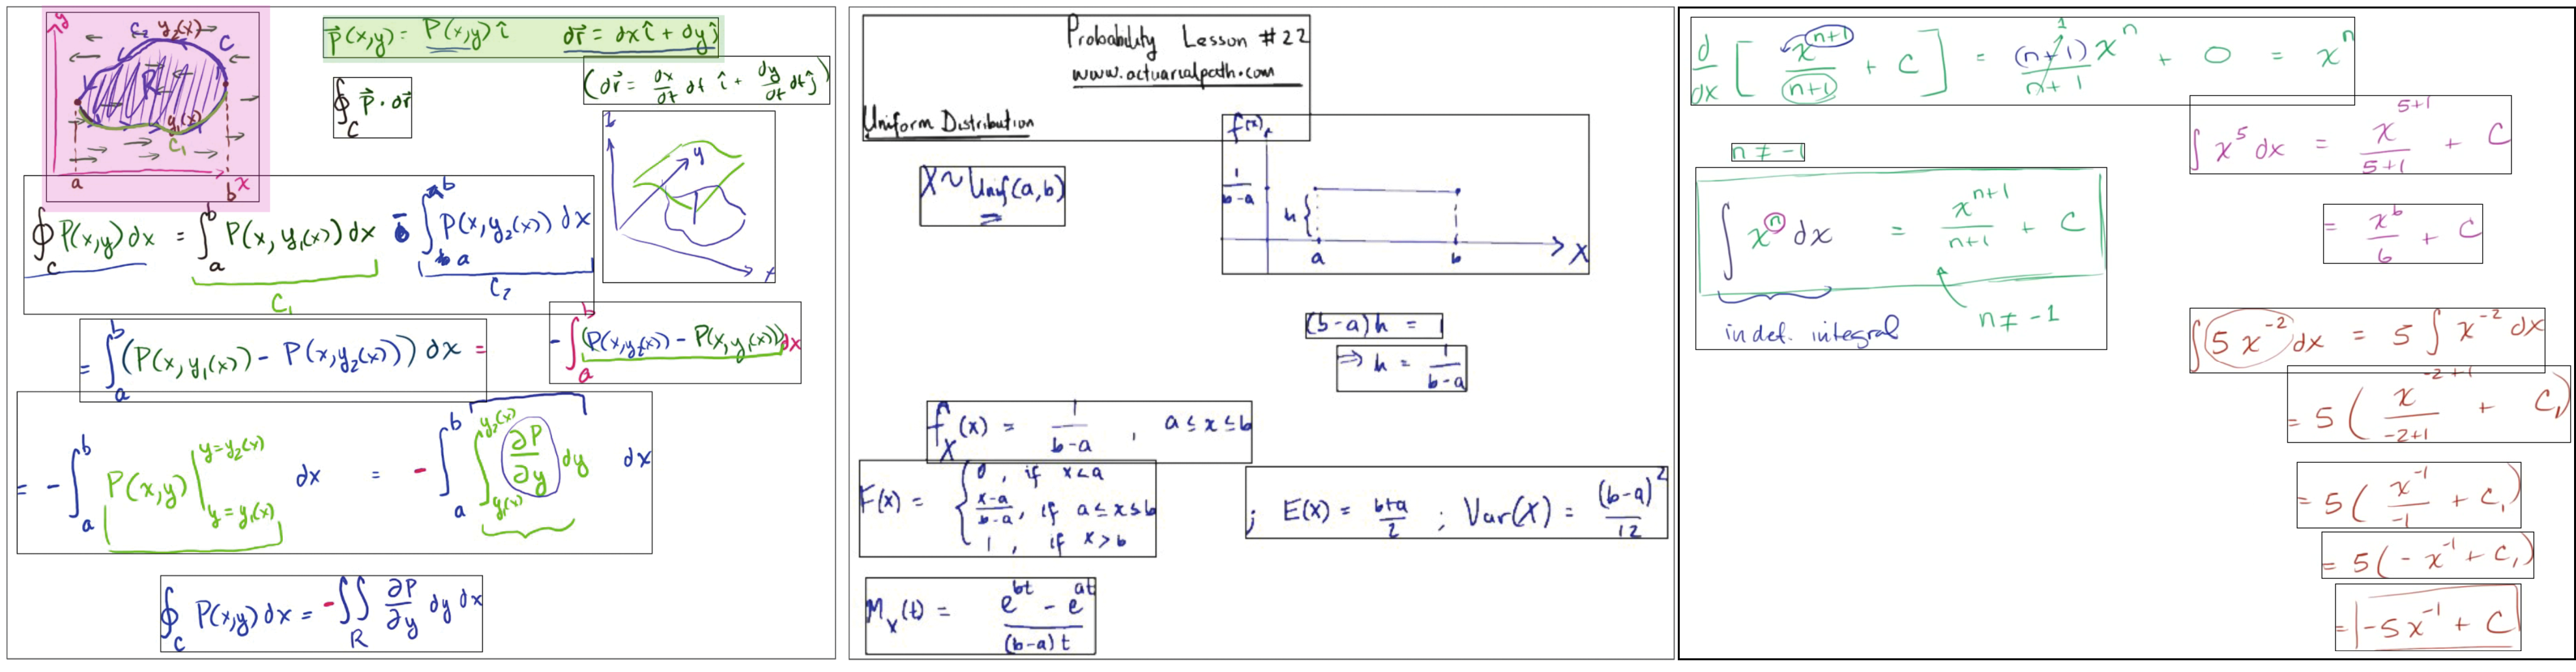
\includegraphics[width=\textwidth]{figures/visual-lines2.pdf}
        \captionsetup{font=footnotesize}
        \caption{Examples of visual entities output from our line-breaking algorithm.
Our algorithm successfully identifies meaningful groups even from complex
layouts with a mix of equations, figures and graphs.}
        \label{Fig:visual_line_output}
\end{figure}
%
To test the robustness of our segmentation algorithm, we applied it to 20 video lectures from 10 different authors, using the same set of parameters as described above. The lectures included nonlinear layouts of visual content and examples of complex diagrams with several layers of information. In all cases, the algorithm produced reasonable segmentations which generated comprehensible \systemname s. There were few cases ($\approx 5\%$) where the output segmentation was less than ideal, but these did not affect the overall quality of the \systemname s. Please see the discussion on section~\ref{sec:discussion} for more details. The full set of results are included in the appendix. 
%---------------------------------------------------
\subsection{Structuring Transcript Content}
\label{sec:text_corr}

Once we have segmented the visual content of the lecture, the next step is to organize the transcript text with respect to the extracted visual entities.
We leverage temporal correspondences between the transcript and visuals to distinguish between explanatory and depictive sentences (section~\ref{sec:principles}) and to break long text descriptions into shorter, more readable paragraphs.

\subsubsection{Aligning transcript to video.} 
To obtain the temporal alignment between the transcript and video, we use an automatic algorithm by \cite{rubin2013content} which extends the Penn Phonetics Lab Forced Aligner (P2FA) built on the HTK speech recognition software. This   aligner takes a verbatim transcript and an audio file as inputs and outputs a time-stamped transcript, where each word is annotated with a start and end time. 

\subsubsection{Detecting explanatory versus depictive sentences.} 
As discussed in section~\ref{sec:principles} about design principles, depictive sentences typically coincide with drawing actions while explanatory sentences do not. Using the time-aligned transcript,
we compute correspondences between transcript sentences and visual entities.
A sentence is matched to a single visual entity if most of its utterance
time ($ \geq 75\% $) overlaps with the drawing time of the visual entity.
If a sentence does not coincide with any entity, we refer to it as an unmatched
sentence. We classify all matched sentences as depictive text (associated with the corresponding visual entities) and all unmatched sentences as explanatory text.
%
Note that while this is a heuristic, we found it to work well in practice. 
%
We use this information in the layout stage to reduce clutter and make the text more readable.    

\subsubsection{Breaking up long text descriptions.}
%
In some cases, complex visual entities that contain a lot of information may get matched with large blocks of depictive text.
%
When reading such text blocks, it can be hard to identify and follow all the correspondences between the individual sentences and the relevant parts of the figure.
%
We address this problem by breaking up complex visual entities into sub-entities, each of which has a shorter, more readable block of depictive text.\\

In particular, we use a variant of the stroke segmentation algorithm described in the previous section to further segment a complex visual entity $e$.
%
In this case, we use the following scoring function $F_\text{sub}$ to evaluate a set of candidate sub-entities, $V_\text{sub}$:
%
\begin{equation} F_\text{sub}(V_\text{sub}) = \sum_{e_\text{sub} \in V_\text{sub}}\lambda_{1}\lvert n_\text{words}(e_\text{sub}) - w \rvert + P_\text{o}(V_\text{sub}) \end{equation} 
%
where $n_\text{words}(e_\text{sub})$ is the number of words in the depictive text associated with sub-entity, $e_\text{sub}$; $P_\text{o}$ is the overlap between bounding boxes of sub-entities in $V_\text{sub}$ (defined in Equation \ref{Eq:overlap_penalty}); $w$ is the target number of words in the depictive text for each sub-entity; and $\lambda_{1}$ determines the relative importance of the word count and overlap terms. We set $w = 50$ (about 2-4 sentences) and $\lambda_{1} = 1/25$.\\

Using this scoring function, we apply the same dynamic programming procedure described in section~\ref{sec:segmentation} to segment $e$ into sub-entities. In this variant, we only allow consecutive strokes to be grouped together since our goal is to obtain temporally sequential sub-entities. Figure~\ref{Fig:videonote_expanded} shows an example output from this optimization.  
%-----------------------------------
\subsection{Layout and Formatting}
\label{sec:layout}
We organize the visual and audio content into a static, sequential format by interleaving visual entities with blocks of transcript text in the order of their appearance in the video. As we point out in section \ref{sec:segmentation}, a single visual entity can be composed of non-contiguous groups of strokes. For example, in Figure~\ref{Fig:line_order}, $e_1$ and $e_2$ each consist of 4 separate groups of strokes, (1\&2, 4, 6, 8) and (3, 5, 7, 9) respectively. In this case, we show each contiguous group of strokes at its associated time, together with previous strokes in the same visual entity which are shown for context. So Figure~\ref{Fig:line_order} would be presented as: 1\&2, 3, (1\&2)\&4, (3)\&5 etc., where the parentheses indicate previous strokes. The new group of strokes is highlighted with color on top of the previous strokes (Figure~\ref{Fig:layout_line_order}). 
\begin{figure}[h!]
        \centering
        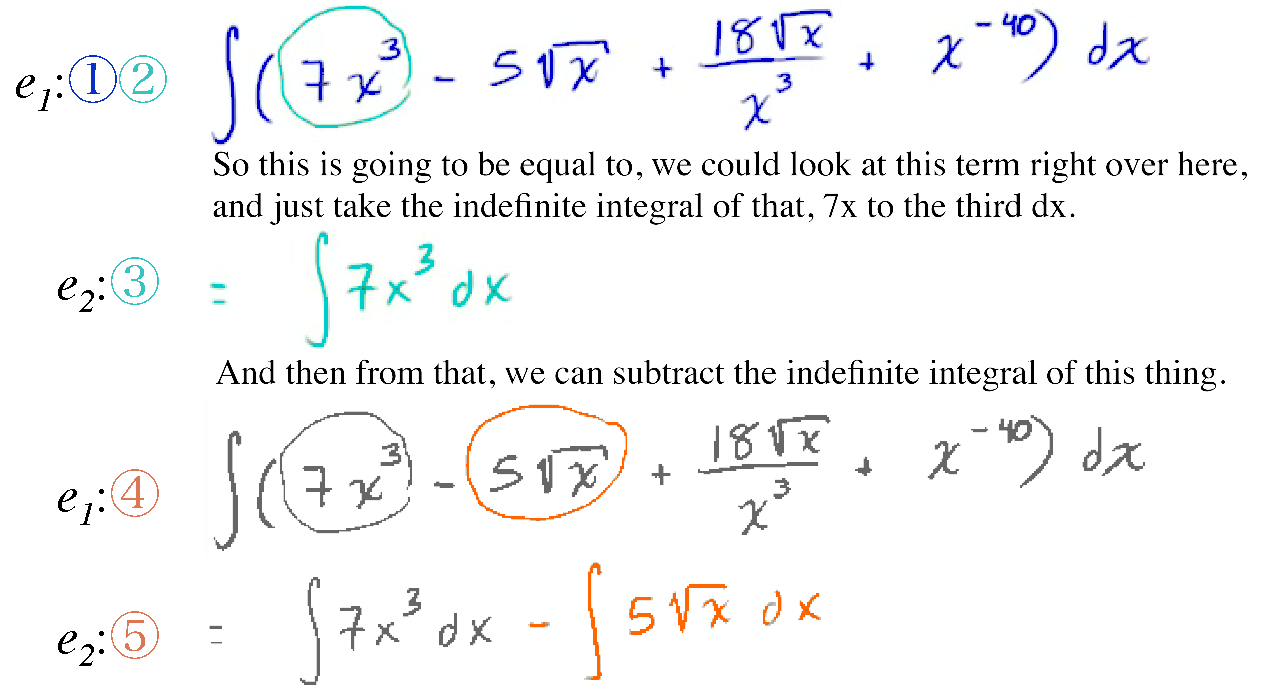
\includegraphics[width=0.8\textwidth]{figures/layout_line_order.pdf}
        \captionsetup{font=footnotesize}
        \caption{\systemname\ presentation of strokes 1-5 of Figure~\ref{Fig:line_order}. Each contiguous group of strokes is shown together with previous strokes in the same visual entity.}
        \label{Fig:layout_line_order}
\end{figure}\\

By default, all visual entities and explanatory sentences are shown; the depictive text associated with visual entities is hidden to reduce clutter. Users can click on the \emph{expand} buttons next to individual visual entities to display the corresponding depictive sentences. For complex visual entities, the expanded view shows the decomposed sub-entities with their associated depictive sentences (Figure~\ref{Fig:videonote_expanded}).\\

%----------------------------------------------------------------------------------------
\section{User Evaluation}
\label{visualtranscript-usereval}
%
\begin{figure*}[h]
    \centering
          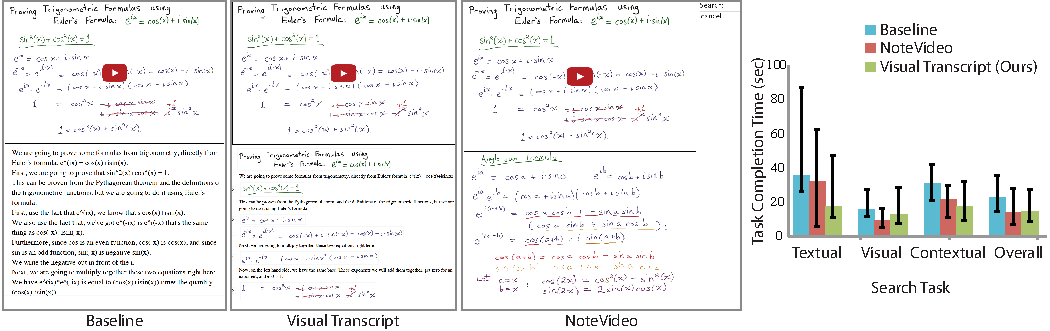
\includegraphics[width=\textwidth]{figures/evaluation-interfaces.pdf}
         \captionsetup{font=footnotesize}
         \caption{(left) We compared three interfaces to study video lectures: A standard YouTube player with an interactive transcript, our VisualTranscript, and NoteVideo. (right) Graph shows median search task completion time, where error bar represents interquartile range.}
    \label{Fig:interfaces}
\end{figure*} 
%
We performed a comparative study to test the hypothesis that \systemname\ facilitates learning. We compared three interfaces to study video lectures: a standard YouTube player with an interactive transcript (Baseline), Monserrat et al.'s interface \cite{monserrat2013notevideo} (hereafter referred to as \textbf{NoteVideo}), and our \systemname\ interface linked to the video (Figure~\ref{Fig:interfaces}). The YouTube video player is currently the most common viewing interface for online lectures, and NoteVideo while less established, was specifically designed to facilitate navigation of blackboard-style lecture videos. In NoteVideo, a panoramic image of the board with strokes from the entire lecture serves as an in-scene navigation interface. Users can click on any stroke to play the video at that point in time.
%
\subsection {User Tasks}
Our study includes two tasks: (1) summarization, to get a quick and comprehensive overview of the lecture without watching the entire video, and (2) search, to quickly locate specific information.
Although not a direct measure of learning, these tasks are inherent activities in learning and also match common evaluation tasks used in the literature on tools for lecture videos \cite{kim2014data,pavel2014video,monserrat2013notevideo}.\\
%
\subsubsection{Summarization Task}
Users were asked to quickly provide an overview of the lecture without watching the entire video. We gave users only 3 minutes to view and summarize 7-8 minute long lectures. We purposely did not give enough time to watch the entire video so as to motivate the users to quickly scan through its content. Before the task, users watched a sample lecture video and read a sample summary comprised of main points and detail points. Users were encouraged to try to write down at least all the main points of the lecture, and as many of the detail points as possible.\\
%
We compared the summaries written by users to a \text{gold standard} list of main/detail points manually created by two referees. The user summaries were scored by the number of points they covered.
%
\subsubsection{Search Task}
The search task emulates scenarios when the user wants to quickly find a specific piece of information in the video (e.g. to solve a question in a problem set, or to look up a specific formula). We differentiate three different types of search problems 
depending on whether the information is in the visuals, the transcript or a combination of both.\\ 

The \textbf{visual search} reproduces situations when a user remembers something visually and wants to find where it appeared. (E.g., \textit{Find the point in the lecture where the instructor strikes out part of an equation, where terms add up to eliminate each other.}) For the \textbf{textual search}, the cue is often a word or a phrase that could be found in the transcript either directly or indirectly (E.g., \textit{Find the point in the lecture where the property that every continuous function has an antiderivative is stated.}) For the \textbf{contextual search}, the information is neither in the text nor visuals alone, but rather in the context between the two. (E.g., \textit{Find the point in the lecture where the instructor writes an integral expression for a bounded area under some curve.}) User performance was assessed by the task completion time as well as correctness.\\

Nine participants (2 female, 7 males), ages 20 to 35 took part in our study. 
All of them were familiar with the general subject matter of the lectures, although they had not seen the particular lectures before.\\

We chose three college-level math lectures for our study: \textit{Fundamental Theorem of Calculus} by Salman Khan (8 minutes), \textit{Proving Trigonometry Formulas Using Euler's Formula} by Lee Stemkoski (7.2 minutes), and \textit{Uniform Distribution} by Actuarialpath (8 minutes).\\
We used a within-participant design, where each participant performed tasks on each interface. We counter-balanced the order of the interfaces and the assignment of videos to interfaces using a Latin Square.\\

Before using each interface, participants were briefed about their features and given time to familiarize themselves. After each task, they answered questions about their interaction with the interface. After completing all tasks, participants completed a questionnaire on their preference and the usability of each interface. Please refer to the appendix for the full set of tasks and post-task questionnaires.
%--------------------------------------
\subsection{Findings and Discussion}
There are several notable findings from our user study:

\subsubsection{Users write more comprehensive summaries with \systemname .}
Users listed the most number of main and detail points using our interface,
although differences across the interfaces were not statistically significant
according to the one-way analysis of variance (ANOVA) (main points:
$F_{2,24}=0.23$, $p=0.79$, detail points: $F_{2,24}=0.48$, $p=0.62$). Table~\ref{Tab:summary_results} shows the percentage of main/detail
points covered by user summaries with each interface.

\begin{table}[!h]
 \centering
 \begin{tabular}{ l |c c c}
 \hline
    & \textbf{Baseline} & \textbf{NoteVideo} & \textbf{Ours} \\\hline
   \textbf{Main points} & 0.83$\pm0.12$ & 0.81$\pm0.21$ & 0.87$\pm0.18$\\
   \textbf{Detail points} & 0.50$\pm0.22$ & 0.56$\pm0.18$ & 0.58$\pm0.15$\\
   \hline
 \end{tabular}
         \captionsetup{font=footnotesize}
 \caption{Percentage of points covered by user summaries compared to the
golden standard list.}
 \label{Tab:summary_results}
\end{table}

Note that while on average, there may not seem to be a significant difference
between ours and the two alternatives, summary quality varied
significantly depending on the video. In particular, when the sequence of lecture was not clear in the panoramic image, NoteVideo users mixed the order of points or missed a main point entirely. For example, in the lecture on \textit{Fundamental Theorem of Calculus} (Figure~\ref{Fig:key_ideas} bottom), NoteVideo users immediately clicked on the ``Fundamental Theorem'' (\raisebox{.5pt}{\textcircled{\raisebox{-.5pt} {4}}}) skipping the first third of the lecture about the graph of a continuous function and the area under it (\raisebox{.5pt}{\textcircled{\raisebox{-.5pt}
{1}}}-\raisebox{.5pt}{\textcircled{\raisebox{-.5pt}
{3}}}). While users performed comparably with \systemname\ or the baseline, when asked which interface they preferred for the summary task, they preferred NoteVideo (5/9) and ours (4/9). 

\subsubsection{Users find information involving text faster with \systemname\ than with NoteVideo or the baseline.}
For the \textit{text search} and  the \textit{contextual search} users performed fastest with \systemname\  followed by NoteVideo and then the baseline (Figure~\ref{Fig:interfaces}right), although the differences across the interfaces were not statistically significant according to the non-parametric Kruskal-Wallis Test ($\chi^2=0.82$,
$p=0.676$).\\ 

For these tasks, users either had to find relevant text or find a visual and also look at the text around it (or listen to the audio). \systemname\ naturally supports such tasks by  interleaving text and figures. NoteVideo does not provide a text to skim through, but users could search for key words or phrases (a feature also provided in \systemname\ and the baseline). Alternatively, they could click on a visual and listen. Interestingly, the baseline performed worst on these tasks, despite the fact that it is most text-centered and  provides the exact same text as \systemname . This is likely because the text in the baseline was unstructured and difficult to read (see next finding).\\

For the \textit{visual search} users performed fastest with NoteVideo. For
all videos we tested, NoteVideo had the advantage of presenting all the visuals
in one screen, which made it easier for users to scan the entire visual content
without having to scroll.\\

On average, participants' performance on the search task was comparable on
ours and NoteVideo, which was better than the baseline. The difference between
ours and the baseline was statistically significant with the Mann-Whitney
U (MWU) test ($Z=-2.1$, $p=0.02$), whereas the difference between ours and
NoteVideo was not ($Z=1.2$, $p=0.12$). Occasionally, users missed the information in their first search attempt and  then tried to scan the entire lecture, contributing to a large variance.\\

In terms of accuracy, users were most successful in locating the correct information with \systemname\ (average error rate $e=0.06$) compared to NoteVideo ($e=0.07$) or the baseline ($0.15$), although the differences were not statistically significant (ANOVA, $F_{2,24}=1.04$, $p=0.15$).

\subsubsection{\systemname\ makes the transcript text easy to read and skim through.}
Both the baseline and \systemname\ include the entire transcript text. However,
the usefulness of their transcripts is rated very differently. On a 1-7 usefulness
scale, \systemname\ scored 6.3 (range: 5 to 7), whereas baseline scored 4.7
(range: 1 to 7). With the baseline, participants mostly scrubbed
through the timeline to complete the tasks. Several users (3/9) mentioned
that the baseline transcript text was difficult to skim through or find correspondences
with the video. In contrast, with \systemname , users primarily relied on
the text and visuals to solve the tasks rather than the video. One user
commented that the layout was \textit{``similar to a textbook''} and \textit{``easy
to read''}. Another user said that \textit{``the paragraph structure corresponds
to the main points''} which facilitates skimming.

\subsubsection{Users prefer \systemname\ for learning.}
The post-task survey showed that, for learning in general, most users (7/9) preferred our interface over NoteVideo (2/9) or the baseline. 
The reasons for preferring \systemname\ included \textit{``having the whole script and equations [visuals]''} and \textit{``a good balance between getting the overview and some more detail.''} Those who preferred NoteVideo appreciated having all visual content presented \textit{at once} without having to scroll, but also noted that the sequence was not apparent (e.g., many users asked where to click to get to the beginning of the lecture) and that \textit{``there's a risk of missing something that's not written on the board.''}\\
%----------------------------------------------------------------------------------------
\section{Discussion}
\label{sec:discussion}
\subsection{Limitations}
\systemname\ focused on blackboard-style lectures, but the key ideas behind the design of \systemname\ (e.g., presenting discrete visual entities next to its corresponding narrative in a linear layout) are generalizable to other style of lecture videos. Different styles of lecture videos would require different or more sophisticated visual entity recognition and layout techniques. For example, a classroom recording might have human occlusion, and a slide-based presentation could have animation or other multimedia effects.\\

The pre-processing step for stroke extraction works especially well with digital blackboard-style lectures with constant background and minimal occlusion. However, videos with more noise (e.g., from lighting change or occlusion by hand) may require a more sophisticated method. We also do not handle special cases
such as partial erasure or copy-and-paste.  For instance, if the instructor
updates a part of visual content in order to correct a mistake, the current
implementation only shows the \textit{newest} stroke.\\

Although in all of our examples the segmentation algorithm outputs produce a comprehensible \systemname , we also observed 2 types of failure cases: (1) \textit{under-segmentation}, where too many strokes are grouped into a single visual entity, and (2) \textit{over-segmentation}, where related strokes are separated into different visual entities. Our scoring function assumes a layout where distinct visual entities are more or less spatially separate from each other. A different method may be required to handle videos that violate this assumption, for example a history lecture where most of the writing is on top of a map, or where figures are overlayed on top of each other (Figure~\ref{fig:humanities_lec}).  An editing or annotation mechanism, including crowdsourcing, to aid segmentation would be useful and a potential area for future work.\\
%
\begin{figure}[h!]
        \centering
        \includegraphics[width=\textwidth]{figures/humanities_lec.pdf}
                \captionsetup{font=footnotesize}
	\caption{Our segmentation algorithm assumes that distinct visual entities are more or less separate from each other. For example, a history lecture
where most of the writing is on top of a map, or where figures are overlayed
on top of each other may require a different method. }
        \label{fig:humanities_lec}
\end{figure}
%

In placing temporally aligned visuals and sentences next to each other, we assume that instructors talk about what they are drawing at the same time. This assumption holds in most cases, but fails to resolve other types of references. For example, in Figure\ref{fig:gesture}, the pronoun `here' is used twice, each time referring to a different part of the visual. Whereas in the video these references become clear with the cursor movement, they remain ambiguous in our static output.

\begin{figure}[h!]
        \centering
        \includegraphics[width=2.2in]{figures/gesture.pdf}
                \captionsetup{font=footnotesize}
	\caption{Layout using only temporal correspondence fails to resolve some references. In this example, `here' in the first sentence refers to the top right portion of the boundary R, whereas the second `here' refers to the bottom left portion. In the video, these references are clarified by pointing with a cursor.}
        \label{fig:gesture}
\end{figure}

%\begin{figure}[t!]
%        \centering
%        \includegraphics[width=\textwidth]{images/gesture.pdf}
%        \caption{\VEDIT{Layout using only temporal correspondence fails to resolve some references. In this example, `here' in the first sentence refers to the top right portion of the boundary R, whereas the second `here' refers to the bottom left portion. In the video, these references are clarified by pointing with a cursor.}}
%        \label{fig:gesture}
%\end{figure}

%\begin{figure}[h!]
%        \centering
%        \includegraphics[width=\textwidth]{images/humanities_lec.pdf}
%        \caption{\VEDIT{Our segmentation algorithm assumes that distinct visual entities are more or less separate from each other. For example, a history lecture
%where most of the writing is on top of a map, or where figures are overlayed
%on top of each other (Figure~\ref{fig:humanities_lec}) may require a different method. }}
%        \label{fig:humanities_lec}
%\end{figure}

\subsection{Conclusion}
This chapter introduced \systemname , a readable and interactive representation of blackboard-style lecture videos, which interleaves visual content with corresponding text. We use a variant of the classic line-breaking algorithm to segment the visual content of a lecture video into discrete figures. Then, we leverage the temporal correspondence between the figures and transcript sentences to structure the transcript text. Finally, we interleave the figures with corresponding text in an easy-to-read format. User evaluation suggests that compared to a standard video player and a state-of-the-art interface for watching blackboard-style lectures, users prefer our interface for learning. It also suggests that \systemname\ is effective in helping users browse or search through lecture videos. 

 % Chapter 2
\cleardoublepage
%% Chapter 3
\newcommand{\voicescript}[0]{VoiceScript}
\chapter{Authoring Voice Recordings} % Chapter title
\label{ch:voicescript} % For referencing the chapter elsewhere, use \autoref{ch:mathtest}

%----------------------------------------------------------------------------------------
% Abstract
%----------------------------------------------------------------------------------------
\section{Introduction}
Audio recordings of speech are prevalent across a variety of media, including podcasts, audio books, e-lectures and voice-overs for narrated videos.
%
Creating such audio recordings typically involves three main tasks: writing a script, recording the speech, and editing the recorded audio. 
%
While authors typically start by writing at least a rough script of what they plan to record, in practice, the process of creating the final audio rarely involves a simple linear progression through these steps. A more common workflow is to move back and forth between writing or editing the script, recording or improvising subsets of the speech, and editing together portions of multiple recorded takes.\\

For example, consider the case of recording the audio for an online lecture. After writing some notes to use as a rough script, the lecturer records a few takes and listens to the speech. She decides that one of the concepts requires a more detailed explanation, so she edits her notes, re-records the relevant speech, and merges the new recording into the final audio. Such updates may also happen in response to feedback from viewers after the lecture is published online. Similarly, when authoring a voice-over for a video, the initial recording may not align perfectly with the visual footage (e.g., some spoken explanations may be too short or too long for the corresponding video clips). In a collaborative scenario, an \textit{editor} could request edits to the initial recording of a \textit{narrator}. In each case, users may need to modify the script and re-record certain sections of the speech. In general, the process of recording and editing the speech together often reveals issues that require going back to edit portions of the script.\\

Unfortunately, most existing tools for authoring speech recordings do not facilitate this back and forth workflow. Typically, users write and edit the script in a text editing environment and then record and edit the audio in a standard waveform editing tool. The central issue  is that the written script and the recorded audio are treated as completely separate entities.
%
This separation introduces several sources of friction in the workflow. When the user records the speech, any deviations from the initial written text (either intentional or not) are not reflected in the script. Evaluating the recordings to decide what takes to choose or what script modifications are necessary requires careful scrubbing through the audio to find the relevant parts. In addition, once the user chooses a particular version of the speech to include, the script no longer matches the speech, which complicates any subsequent edits. Finally, if the user decides to modify a portion of the script, she must figure out what subset to re-record to ensure that the new recording can be merged in without creating audio artifacts (e.g., replacing a single word in a recorded sentence is hard to do since the word may not blend seamlessly with the adjacent words).\\

To address these challenges, we design \voicescript\, an interface that supports script writing, speech recording, and audio editing in a unified way. Our key idea is to maintain a so-called \emph{master-script} that is linked to the audio and always reflects the current state of the project, including unrecorded, recorded, improvised and edited portions of the script. We use automatic speech recognition to transcribe the audio into text, and solve the task of combining together multiple recordings and syncing audio with the script like a text differencing and merging problem. To help users maintain a consistent master-script, \voicescript\ provides semi-automated tools for merging recorded takes into the master-script and visualizations that indicate what portions of the script need to be recorded (or re-recorded) in response to edits to the script. The combination of these features enables users to move back and forth between script editing, speech recording and audio editing in a seamless fashion.\\

\voicescript\ can be used to create audio recordings in a variety of workflows, including recording a fairly detailed script, recording without any script, and a collaborative scenario between two
users. We conduct informal evaluations where users create their own audio recordings to summarize technical articles. We also compare \voicescript\ to a state-of-the-art text-based audio editing tool for the task of creating an audio recording from multiple raw recordings. The results demonstrate that \voicescript\ supports a wide range of workflows and enables first-time users to  easily author speech recordings. User feedback suggests that the integration of script and audio through the master-script greatly facilitates the authoring process. 

%----------------------------------------------------------------------------------------
\section{Previous Work}
\subsection{Scripting}
Adobe Story \cite{adobestory2016}, FinalDraft \cite{finaldraft2016} and Celtx \cite{celtx2016} are examples of professional software dedicated to script writing. They support collaboration, automatic formatting, navigation and planning for future production, but they treat the script as a text document that is essentially separate from the recordings. In fact, in our formative interviews of lay and professional audio producers, we found that many of them use general-purpose document editors like Google Docs \cite{googledocs2016} or Microsoft Word \cite{microsoftword2016} to prepare their scripts.

\subsection{Recording and Editing Audio}
At the recording and editing stage, many users rely on commercial digital audio workstations, like Adobe Audition \cite{adobeaudition2016}, Avid ProTools \cite{avidprotools}, GarageBand \cite{garageband} and Audacity \cite{audacity}. Video editing software such as Adobe Premiere \cite{premier} or ScreenFlow \cite{screenflow} are also commonly used. These tools allow users to edit audio by manipulating waveforms in a multi-track timeline interface. They also provide a wide variety of low-level signal processing functions. However, since they are designed to serve as general-purpose audio production systems, they include many features that are not directly relevant for creating audio narratives whose main content is speech. Hindenburg Systems \cite{hindenburg} develops tools that are specifically targeted for audio narratives. Still, they are primarily concerned only with the audio and they do not deal with the script directly.   

\subsection{Text-Based Audio Editing}
Recently, several researchers have explored using audio transcripts to support text-based navigation and editing of audio. Whittaker and Amento \cite{whittaker2004semantic} demonstrate that users prefer editing voicemail through its transcript instead of its waveform. Inspired by similar intuition, Casares et al. \cite{casares2002simplifying} and Berthouzoz et al. \cite{berthouzoz2012tools} enable video navigation and editing through time-aligned transcripts. Rubin et al. \cite{rubin2013content} extend this approach to audio narratives and propagate edits in the transcript text to the corresponding speech track. These systems all focus on editing pre-recorded audio via its transcript, whereas we also consider how script edits influence the recording process and how audio edits also evolve the script.\textit{NarrationCoach} developed by Rubin et al. \cite{rubin2015capture} also uses automatic speech recognition to align speech recordings with an input script. However, its focus, improving speech performance at recording time, is different from \voicescript. Here, we focus on facilitating the back-and-forth workflow between script writing and speech recording.\\
\voicescript\ also takes advantage of text-based navigation and editing, but unlike these systems, it supports a dynamic workflow where both the audio recordings and the underlying script can be continuously updated.      

%----------------------------------------------------------------------------------------
\section{Design Principles}
To learn about current practices and challenges for creating speech recordings, we interviewed ten professional lecturers and two video producers who regularly create audio recordings for online lectures that are published on online platforms, including YouTube, Udacity, EdX and MITx. The following are several key insights we gained from the interviews.\\

\paragraph{Scripts are prevalent.} All of the lecturers prepared written materials about what they were going to say before they started recording. The format and level-of-details of these scripts varied. For instance, one lecturer used his lecture slides containing images and a list of bullet points as his script. Another lecturer typed a thorough word-for-word transcription of what he was going to say in a text document. Another person used handwritten notes as an outline. In all cases, while they were recording, they kept the scripts within their view and depended on them to guide their speech.  

\paragraph{Recordings deviate from the script.} In many cases, the initial scripts were rough or incomplete. Only two out of the ten lecturers we interviewed prepared a word-for-word script before recording. The majority used lecture slides or handwritten notes containing a rough outline of what they were going to record. They used these outlines as guides and improvised most of the actual recorded speech. One of the lecturers did an initial recording from the outline, and then used that to flesh out the script before recording additional takes. Even when a word-for-word script was prepared beforehand, the recording often did not follow the script exactly. While recording, the speaker sometimes remembered and added more details, or found a more natural way of saying a written sentence. In some cases, major script changes were made long after the initial recording was created. For example, one lecturer noted that he periodically revisited and re-recorded parts of lectures to add up-to-date examples. The result is that recorded speech almost always differs either slightly or significantly from the initial written script. \\
While a few people edited the written script to resolve these discrepancies, in most cases the script and recorded audio end up in inconsistent states. This inconsistency makes it difficult for users to update the recording. They cannot simply read and edit the script because it may not accurately represent the recorded audio. Moreover,  changing any portion of the recording requires identifying the appropriate subset of speech to re-record such that the new recording can be merged into the final track with no noticeable seams at the take boundaries.  

\paragraph{Final track includes multiple recordings.} As mentioned above, users almost always record multiple takes of the speech. Thus, assembling the final track typically requires merging these takes together using audio editing software. Many users noted that aligning the waveforms of multiple takes, finding the best take, and then cutting and joining them seamlessly were very time consuming and tedious tasks.

%----------------------------------------------------------------------------------------\
\section{The \voicescript\  Interface}
Based on these observations, we designed \voicescript\, a speech authoring interface that supports script writing, speech recording and audio editing in a single unified workflow. Our interface is built on three key features.

\paragraph{Text-based representation of audio.} We build on previous work~\cite{casares2002simplifying,whittaker2004semantic,berthouzoz2012tools,rubin2013content} that demonstrates the benefits of text-based representations of spoken audio for navigation and editing. \voicescript\ uses automatic speech recognition to transcribe audio recordings in realtime and represent each take with a verbatim transcript. As with previous systems, edits to these text transcripts are automatically propagated to the audio, which facilitates simple audio editing tasks. 

\paragraph{\emph{Master-script} view.} To help users manage the relationship between scripted text and recorded speech, we introduce the notion of a \emph{master-script} that shows a unified view of both unrecorded portions of the script and recorded speech included in the final track. By representing and visualizing both recorded and unrecorded text, the master-script provides a complete, readable view of the current state of the project that evolves as the user records and adds new takes to the final track, edits recorded text, or adds/modifies text that must be recorded. 

\paragraph{Merge process.} Since recorded text typically differs from the script, \voicescript\ provides an interface for merging changes into the master-script. The fact that we represent all recorded audio as text allows us to use standard text differencing to identify conflicts and execute merges. One key difference between our scenario and standard text merging is that recorded audio cannot simply be cut and merged into the master-script at any arbitrary word boundary. In many cases, the temporal gap between spoken words is not big enough to produce a seamless edit in the final track. Our merge interface takes this into account and helps the user execute merges that are likely to be artifact-free.\\

The rest of this section describes our interface through typical usage scenarios of how users might create an audio recording. 
%
\subsection{Typical Usage Scenarios}
%
\begin{figure}
  \centering
  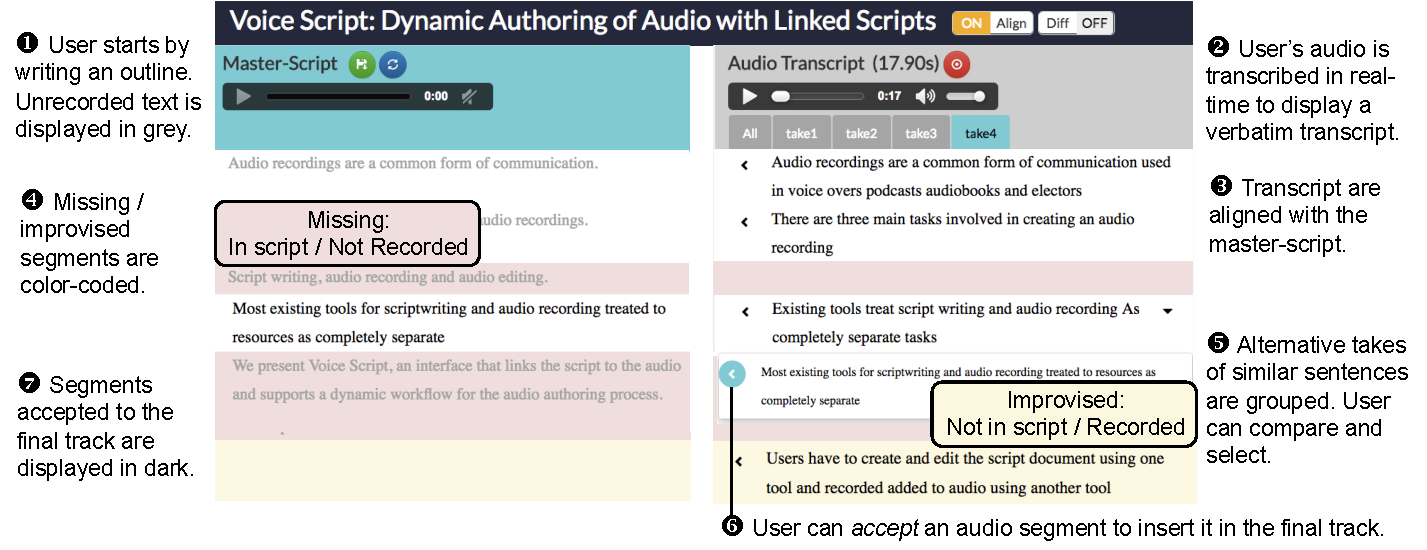
\includegraphics[width=\textwidth]{figures/ui_aligned2}
  \caption{The \voicescript\ interface. The \textit{master-script} view on the left shows the current state of the project, including both recorded and unrecorded text. On the right, there are individual tabs for each recording, along with an \textit{All} tab that shows a summary of all takes.}~\label{fig:ui_aligned}
\end{figure}
%
The rest of this section describes our interface through typical usage scenarios of how users might create an audio recording. 

\subsubsection{One-pass authoring.} 
Typically, the user begins by writing an outline of points to record in the master-script.
The text appears in light grey to indicate that these parts have not been recorded yet (Figure~\ref{fig:ui_aligned} \textit{left}). At this stage, the master-script is like an ordinary, editable text document. \\

Once the user starts recording, the audio is transcribed in real time and verbatim text corresponding to each take appears in a separate transcript tab (Figure~\ref{fig:ui_aligned} \textit{right}). Each transcript is time-aligned with the corresponding recording, so the user can quickly navigate to specific
parts of the audio by clicking on a word in the transcript. \\

The next task is to cut and merge parts of the recording into the final track. The user needs to compare the recording to the original outline, replace parts of the outline with the corresponding recording, and/or insert improvised speech. To this end, we provide a \textit{compare-view} that aligns segments of the recording transcript to corresponding segments in the master-script and shows them side-by-side. To indicate improvised portions of the audio, any segment of the transcript that does not correspond to any part of the master-script is highlighted in yellow. To indicate missing portions in the audio, any segment of the master-script that does not correspond to any part of the transcript is highlighted in red. To
view more detailed discrepancies between the script and recording, the
user can enable a \textit{diff-view} that displays per-word differences
using standard track change markers (i.e., strikethroughs for
missing words and highlighting for added words). \\

To add recorded audio to the final track, the user can \textit{accept} any portion of the recording by clicking a button next to the appropriate transcript segment. If there is a corresponding segment in the master-script, the accepted transcript segment replaces it. If there is no corresponding master-script segment, the accepted transcript segment is simply inserted into the master-script. Within the master-script, accepted segments appear in black to indicate that these are recorded portions of text that have been added to the final track. \\

If the user records more than one take, the user has to compare and select between multiple versions of the same segment. In addition to each of the transcript tabs, the \textit{all} tab provides a summary of all of the takes. For each segment in the master script, this tab displays all the corresponding transcript segments from all of the audio takes. A drop-down button next to a transcript segment  indicates that there are multiple versions (or takes)  of the  segment. Clicking on the button opens a list showing the alternative versions (Figure ~\ref{fig:ui_aligned}-5). The user can listen to any of these takes and select one without having to search through individual takes. \\

Finally, the user has to determine which parts of the outline is still missing. When the \textit{all} tab is in focus, any part of the master-script that has not been recorded in any of the takes is highlighted in red. In this way, the user can tell at a glance what has already been recorded and what still needs to be recorded. All of the dark (i.e. recorded) text in the master-script represents the current state of the final audio track; all of the grey text has not been recorded or is recorded but the author has not yet accepted it into the final track. 

\subsubsection{Iterative and collaborative authoring.} 
The final recording is rarely produced in a single pass. Instead, the user often iterates back
and forth between editing the master-script, recording audio takes, and merging
audio segments into the final track. It is also common for multiple people to collaborate on a single voice-over. For example, a narrator who records the voice-over may work with others who write/edit the script, or several people may work on a recording with multiple voices. \\ 

During any point in the process, users can edit the master-script
like a text document.  For example, a user can simply insert
more text to record or make changes to unrecorded text to flesh
out the original outline. These edits can include verbatim script as well as comments or stage directions (e.g., "include examples" or "speak softer").
A user can also edit or delete recorded portions of the text. Deleting recorded text from the master-script will remove the corresponding portion of the audio from the final track. Altering recorded text can introduce audio artifacts (e.g., when a word is deleted mid-sentence), or it could mean that the corresponding text no longer match the underlying audio. When the user edits a recorded word without completely deleting it, the word is flagged as \textit{dirty} (italicized and marked blue) to remind the user to review or re-record relevant portions. Finally, the user has an option to correct the transcription of recorded words without affecting the underlying audio or flagging it as \textit{dirty}.\\

In both iterative and collaborative editing, users need to identify (1) new content that needs to be recorded for the first time, and (2) existing content that needs to be re-recorded after the script edits. To visualize this information,  \voicescript\ keeps track of per-word metadata about whether a word is unrecorded (grey), recorded and unedited (black), or recorded and edited (blue italics). For collaboration, this metadata is passed between users with the script and recordings. The visualization and the text-based  editing/merging interface facilitates audio editing even when different persons work on different parts of editing the script, recording the audio and/or re-arranging the recorded audio. \\ 

\subsubsection{Other workflows.} 
One key benefit of our interface is that it supports a wide range of workflows for different users and scenarios. For instance, instead of starting with a written outline, the user can begin with an empty master-script, start recording, and then use  the initial recording as an outline. The user can also record the entire script in a single take, or work on a single section at a time. \\

Please visit \url{https://people.csail.mit.edu/hishin/projects/voice_script/abstract.html} to see a video describing the interface. The voiceover for this video was created by two authors collaborating over \voicescript . We also look at various workflows in our informal user evaluation in Section~\ref{sec:usereval}. 

%----------------------------------------------------------------------------------------
\section{Algorithms}
\label{sec:algorithms}
Our authoring interface relies on audio transcription and text alignment algorithms to link the master-script to the audio recordings.  

\subsection{Transcribing the audio recording}
We use IBM Speech to Text Service \cite{ibmspeechtotext} to obtain a verbatim transcript of each audio recording in real-time. The service outputs a time stamp for each word indicating its start and end time within the audio. It also segments the transcript into \textit{utterances} where each utterance is separated by a longer silent gap in the speech (longer than 500 ms). While automatic speech recognition is imperfect, we have found that in most cases the results were accurate enough for the purpose of alignment (described below) and for users to understand the transcript. 
  
\subsection{Aligning the transcript to the master-script}
To support our side-by-side \textit{compare-view} as well as the \textit{All} tab view, we must identify corresponding parts of the master-script and recording transcripts. Moreover, we must partition these corresponding parts into segments that users can easily compare and merge into the master-script. Ideally, our segments should respect natural boundaries such as punctuations and line breaks in written text to aid readability. As discussed earlier, the segment boundaries should also align with longer pauses in the audio so that merge operations do not introduce obvious audio artifacts. Finally, we also want to separate parts of the transcript that generally agree with the master-script (i.e., planned speech) from parts that do not (i.e., improvised speech).  We designed a scoring function that optimizes for these requirements and use an iterative algorithm to co-segment the two texts. We first explain the algorithm and then describe the scoring function in detail.

\subsubsection{Iterative co-segmentation.}
Before running our co-segmentation algorithm, we first compute the global word-to-word alignment between each recording transcript and the master-script using the Needleman-Wunsch (NW) algorithm \cite{needleman1970general}. NW allows for insertions and deletions, which account for differences in the two texts, for example, due to rough scripts, inaccurate speech, or transcription errors.
%
The segmentation of the master-script depends on the segmentation of the transcript and vice versa. Our iterative algorithm alternates between optimally segmenting the master-script and the transcript independently using the result from one to segment the other. We initialize the segment boundaries at punctuation marks (.!?:;) in the unrecorded text and silent gaps ($>$\ 500ms)\ in the recorded text. In practice, we
found that two iterations were sufficient to converge to a solution.

For each optimization step, we use the classic optimal line-breaking algorithm by Knuth and Plass \cite{knuth1981breaking}: The algorithm takes an input text $T$ and a reference text $R$, and outputs an optimal segmentation for $T$. Given the input text as a sequence of $n$ words $T = \{w_0,\dots,w_n\}$, the algorithm finds the optimal set of inter-word
boundaries that break the text into segments. We refer to the boundary between $w_i$ and $w_{i+1}$ as $b_i$.
%
The algorithm iterates through each word, and for each $w_i$
computes and records the optimal set of text segments $S_i$ for words up to $b_i$, along with the total score $E(S_i)$ of
this partial solution. $S_i =\{s_0, ... s_i\}$ is a sequence of segment labels, where $s_i$ is the index of the segment that word $w_i$ belongs to. To determine the optimal partial solution for $w_i$, it
considers each previous boundary $b_j$ $(j<i)$, and evaluates two possible ways of
segmenting the text $T_{ji} = \{w_\text{j+1},
\dots,w_\text{i}\}$: (1) appending $T_{ji}$ to the last segment in $S_j$, or (2) forming a new text segment with $T_{ji}$. The algorithm selects the better (lower) of the two scores for $T_{ji}$ and adds it
to $E(S_j)$ to obtain the total score for the proposed
segmentation. After considering all candidate boundaries $b_j$, the partial solution with the minimum segmentation score is stored as the optimal partial solution. Once the algorithm iterates through all the words, $S_n$ is the
optimal set of segments for the entire text $T$. 

\begin{figure}
\centering
  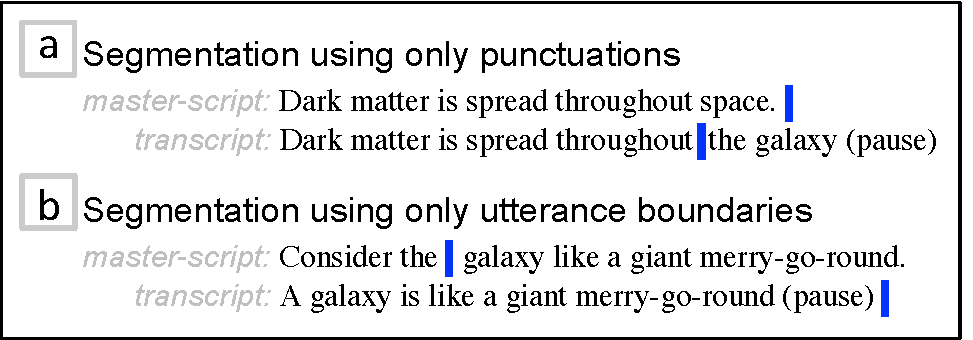
\includegraphics[width=\textwidth]{figures/scoringfunc.pdf}
  \caption{Co-segmentation of master-script and transcript texts. (a) Segmentation using only punctuation marks results in abrupt cuts in the audio. (b) Segmentation using only utterance boundaries produces unnatural cuts in mid-sentence. Our scoring function takes into account both sentence punctuation marks and audio pauses.}~\label{fig:scoringfunc}
\end{figure}

\subsubsection{Scoring function.}
The dynamic programming algorithm described above requires a
scoring function ($E$) that evaluates the goodness of a candidate segmentation. $E$ is a sum of the scores ($e$) for individual segments in the candidate segmentation. We define the scoring function
based on three terms: 
\begin{enumerate}
\item{\textit{Punctuation and silent gaps}: We prefer segment boundaries after sentence punctuation marks, and in case of recorded text, where there is a longer silent gap. Placing cuts at silent gaps allows audio segments from different takes or different parts of a single take to be joined seamlessly. More precisely, we define the boundary score ($e_b$) for a single text segment $T_{ji} = \{w_\text{j+1}
\dots,w_\text{i}\}$ as:
\begin{equation}
    e_b(T_{ji})= 
\begin{cases}
   1.0, \text{ if } w_i \text{ is unrecorded w punctuation (.!?:;)}\\
   -1.0 \text{ if } w_i \text{ is unrecorded w/o punctuation}\\
   t_{gap}(w_{i}) \text{ if } w_i \text{ is recorded} 
\end{cases}
\end{equation}

where $t_{gap}(w)$ is the silence gap in seconds after a recorded word, $w$, and is equal to 1.0 for $w$ that is at the end of a recording.
It is important to consider both the sentence punctuation and the silent gaps. As the examples in Figure~\ref{fig:scoringfunc} illustrate, considering only punctuation can result in audio artifacts when merging recordings. Similarly, considering only utterance boundaries can produce unnatural cuts in the middle of a scripted sentence.
}

\item{\textit{Global alignment}: We try to separate transcript segments that have a counterpart in the master-script (planned) from those that do not (improvised). Likewise, for the master-script, we want to separate segments that have a match in the transcript (recorded) from those that do not (unrecorded). We utilize the global alignment output from the Needleman-Wunsch (NW) algorithm. For each word $w_i$ in the input text ($T$) NW outputs a mapping 
to the reference text ($R$), and vice versa. For instance, $m_i$ is the index of the word in  $R$ that matches $w_i$. $m_i < 0$ if the word has no match. We prefer text segments that have the proportion of matching words close to 0 or 1. The alignment score ($e_a$) for a single text segment $T_{ji}$ is:  
\begin{equation}
e_{a}(T_{ji}) = 2\times\bigg|\sum_{n=j+1}^{i}{match(w_n)}\big/(i-j) - 1/2 \bigg|
\end{equation}
where $match(w_i)$ is 1 or 0, depending on whether $m_i \geq 0$ or not (whether the word has a match or not).
}
\item{\textit{Consistency with the other text}: Since the end goal is to align the segments from both texts, we would like the segment boundaries from the input text to align with the segment boundaries in the reference text even when the punctuation and utterance boundaries do not coincide. Let $S' = \{s'_0, \dots, s'_n\}$ be the segmentation of text $R$. Given this segmentation and the mapping of $T$ to $R$ from NW, the consistency score ($e_c$) for a text segment $T_{ji}$ is:
\begin{equation}
    e_c(T_{ji})= 
\begin{cases}
   1.0, \text{ if } s'_{m_i} \neq s'_{m_k} \text{ for the smallest } k>i, m_k \geq0\\
   -1.0 \text{ otherwise }
\end{cases}
\end{equation}

$s'_{m_i}$ is the index of the segment which $w'_{m_i}$ belongs to and likewise for $s'_{m_k}$. $w'_{m_k}$ is the closest word after $w'_{m_i}$ that has a match in $T$.
} 
\end{enumerate}

We combine these terms into a single scoring function $e$ as follows. 
\begin{equation}
e(T_{ji}) = e_a(T_{ji}) + e_b(T_{ji}) + 0.5  e_c(T_{ji})
\end{equation}
The goodness score for a set of text segments $S$ is:
\begin{equation}
E(S) = \sum_{T_{ji}\in S}{e(T_{ji})} - \big|S\big|
\end{equation}
where $\big|S\big|$ is the number of segments in $S$ and is a normalization term. For notational convenience, we use $T_{ji}\in S$ to refer to the set of contiguous words in $T$ that are assigned to the same segment in $S$. \\ 

We iteratively segment the master-script and the transcript texts. In practice, we found that 2 iterations was sufficient to converge to a final co-segmentation of the two texts.

\subsubsection{Alignment.} 
Given a co-segmentation of the master-script and the transcript text, we then compute the best matching master-script segment for each transcript segment. The match score between two text segments $T_1$ and $T_2$ is defined as the proportion of words in those segments that have a match between each other (from the NW output).
The result is an alignment between the master-script and transcript segments. 

We use this alignment to facilitate syncing and merging of script/audio by presenting tools similar to  common text differencing and merging tools. The \textit{compare-view} displays matching segments side-by-side. Our color-coded visualization indicates which portions of the master-script is missing from the transcript, and which parts of the transcript are improvised (parts that do not have matching segments). In the \textit{all} tab, segments from separate transcripts that match similar portions of the master-script are grouped together so that users can quickly compare and select between one of them. Similar to text or code merging, users can select a transcript segment to overwrite the matching master-script segment.



%----------------------------------------------------------------------------------------
\section{User Evaluation}
\label{sec:usereval}
\subsection{Informal User Study}
To assess the overall usability of \voicescript\ and to observe how users leverage various features of the interface, we conducted an informal evaluation with 4 users (U1-4). We started each session with a 10-minute demonstration of our interface. Then, we gave users a short article about a technical subject: \textit{What
is a Decibel?} from \textit{howstuffworks.com} \cite{howstuffworks} or \textit{How Lasers Work} from
David Macaulay's illustrated book, \textit{The Way Things Work}
\cite{macaulay1999way}. The users' task was to create an explanatory audio recording about the subject using our interface. Users were allowed to refer to the article during the authoring process or to take notes on the master-script, but they were discouraged from recording the article by reading it out loud. We examined the users' workflow and solicited written qualitative feedback about the authoring experience at the end of the session. Each session lasted about 40 minutes.

\subsubsection{Findings}
While the size of our user evaluation is small, the initial findings are extremely encouraging. All users successfully produced a complete audio recording summarizing the article. %(Table 1). 

\begin{mldescription}
\mlitem{\voicescript\ supports various workflows.} Interestingly, each user adapted a very different workflow. For example, U1 started by writing a complete list of main points. For each take, U1 recorded a few points from the list, merged them into the master-script, and then continued to record the next points on a separate take. In contrast, U2 wrote part of the script, recorded that portion, and moved on to write the script of the next part. U3 did not write an initial script, but improvised the recording and used that as a starting point to edit and re-record afterwards. Similar to U1, U4 started by writing a rough outline. But, instead of recording a few points, U4 recorded the full script at each take and merged the best parts to get the final track. Sometimes users typed verbatim script to read aloud during the recording, and other times they wrote rough outlines. For example, U2 noted,  \textit{``For
the introduction, I had a pretty good idea of what I wanted to
say, so it saved me time to use only bullet points. [For the
second part] I wrote full sentences, as I was not familiar with
all the technical details and it would have been more difficult
to improvise. I enjoyed being able to use the master-script in
both ways.''} The differences in the workflows could be due to personal preference, and/or  to the article content. In any case, our interface was able support various workflows. 

\mlitem{The master-script facilitates iterative workflows.} As the above examples also demonstrate, users took advantage of the master-script to go back and forth between scripting and audio recording. For instance, U2 initially wrote a very rough outline for the script.
After recording and merging the first take based on this rough script, U2 refined the master-script, and then recorded more takes. Similarly, after recording and merging audio takes into the final track, U1 noticed a mistake in the speech
(i.e., instead of saying \textit{140 decibels}, U1 had said \textit{40}
decibels). U1 corrected the corresponding recorded text in the
master-script, re-recorded
the relevant portion part by reading out the edited master-script, and replaced it.
During the back-and-forth iteration, users took advantage of our color-coded visualization that indicated sections of the mater-script that required recording  (grey) or re-recording (blue italics). 

\mlitem{Users found the master-script to be helpful.}
All users offered strong positive feedback about our authoring
interface, and said they would use it to create speech recordings. They were most enthusiastic about the integration
of the script and the recordings in the master-script document,
and the ability to align the master-script to the transcripts.
To quote from one user, \textit{``Writing the script on the same interface and having
that integrated with the audio was most helpful.''}  Another user noted
that the \textit{``compare-view helped to keep track of what pieces
of information was already recorded and which ones were still
needed.''} 

\mlitem{Users were satisfied with the final voice-over quality.} 
Participants were satisfied with the overall quality
of the final recording. One user wrote, \textit{``I was surprised
how the final recording from the multiple takes was seamless.''} Users noted that while speech recognition was imperfect, \textit{``the transcriptions were accurate enough to understand and easy to check [by clicking to listen to the corresponding audio].''}
\end{mldescription}
%------------------------
\subsection{Comparative study}
\begin{figure}[!t]
\centering
  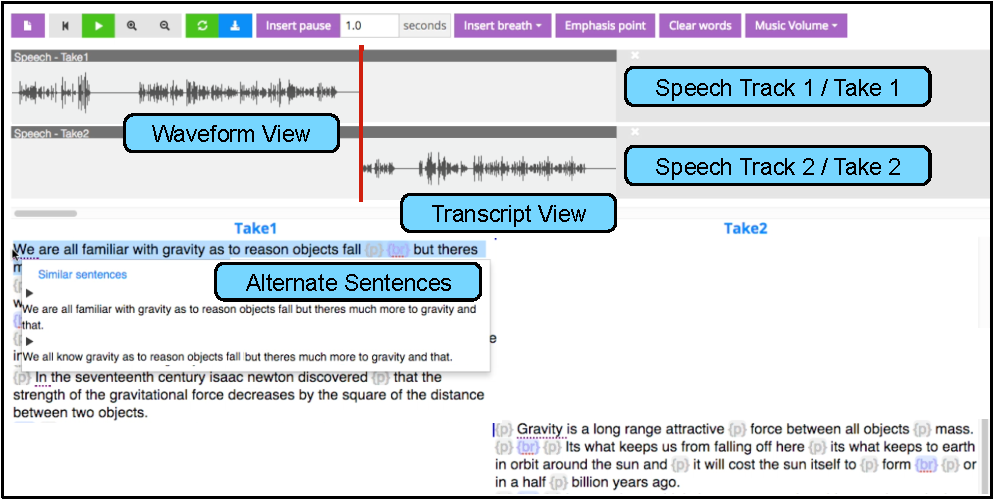
\includegraphics[width=1.0\columnwidth]{figures/interfaceR.pdf}
  \caption{Rubin et al.'s text-based audio editing tool (\textit{Interface-R}). For the purpose of our comparative study, each audio take was loaded as a separate speech track.}~\label{fig:interface-r}
\end{figure}\voicescript

One of the main tasks in creating audio recordings is cutting and merging multiple audio takes. Many existing software specifically assist this task (see Related Work). We separated out this audio editing task, and conducted a small comparative study to explore whether our master-script view facilitates the task compared to a state-of-the-art transcript-based speech editing interface \cite{rubin2013content}. 

Similar to \textit{Voice Script}, Rubin et al.'s interface (shown in Figure~\ref{fig:interface-r}, and referred to as
\textit{Interface-R} hereafter) also uses time-aligned transcripts to support text-based editing. In both systems, users
can edit the transcript like a text document using operations
such as copy-and-paste, insert, or delete, and the edits are propagated
to the audio. Both systems also detect alternate takes of the
same sentence and groups them together so that users can easily compare and select between them.
However, unlike \textit{Voice Script} , Interface-R does not have a master-script that integrates multiple audio recordings with a script. In fact, Interface-R does not explicitly handle multiple recordings. To simulate
multiple recorded takes, we took advantage of their multiple speech tracks,
so that each take appeared in a separate speech track (i.e., separate columns).

We recruited 4 participants, none of whom had
prior experience using text-based audio editing systems. We gave them
a script with bullet points outlining a mini lecture on a technical
subject (\textit{Gravity} and \textit{Dark matter}) and
two audio takes roughly corresponding to the script. In \textit{Voice Script}, the script was contained in the initial master-script. Since Interface-R does not have a notion of
a script separate from the transcripts, we gave users a hard copy
of script. The task
was to cut and merge the two pre-recorded takes to produce a recording that
contained all the contents listed in the script and only those
contents. The two takes were similar, but each take had some
missing content and some extra
content. The participants had to choose parts from each take
and combine them to get the final result. We encouraged the users
to focus on having the complete content rather than on the details
of the audio quality (e.g. tempo, diction, flow of speech).

Each participant completed the task twice, once on each interface using different scripts.
The subject of the lecture and the order of the interface were
counter-balanced. We examined the time users spent to complete the task, the number/type of functions they used, and the quality of the
final recording. After each task, participants gave written
qualitative feedback about their experience. In total, each session lasted about 1 hour. 
\subsubsection{Findings}    
\begin{table}[!t]
\center
\tabcolsep3pt
\begin{tabular}{c|cccccc}
\multicolumn{7}{c}{\textbf{Audio Editing Session}}\\\hline
{User}&\multicolumn{2}{c}{Time spent}& {Total} & {Accept}
&{View}&{Text} \\
{}&\multicolumn{2}{c}{ours \textit{(Rubin)}}&{cuts}&{\textit{ind
/ all}}&{alternate}&{edit}
\\\hline
\textit{A}&\multicolumn{2}{c}{5:58 \textit{(08:10)}}&{3}& {4
/ 3}&{-}&{2}\\
\textit{B}  &\multicolumn{2}{c}{6:40 \textit{(11:10)}}&{3}&{3
/ 4}&{-}&{1}\\
\textit{C}&\multicolumn{2}{c}{9:37 \textit{(11:05)}}&{2}& {7
/ -}&{1}&{7}\\
\textit{D}&\multicolumn{2}{c}{7:25 \textit{(09:10)}}&{6}& {10
/ 1}&{3}&{-}
\\\hline
\end{tabular} 
\label{tab:editing}
\caption{Four participants created audio
recordings from two pre-recorded takes, using our interface and
Rubin et al.'s interface. Usage statistics pertain to our interface.
Accept \textit{ind / all} are number of segments accepted from
the individual transcript view and the \textit{all} tab view
respectively.}
\end{table} 
\begin{mldescription}
\mlitem{Users completed the task faster using Voice Script.} All participants completed the task 25\% faster using our interface (average 7.4  \textit{vs} 9.9 min), and also preferred it to Interface-R. The difference may be explained by the different workflow that each interface affords. In Interface-R, users effectively started with both recordings in the final track. They applied copy-and-paste to cut and merge the two takes, and deletion to remove redundant or superfluous content. In contrast, in \textit{Voice Script}, users started with an empty final track. Then, using the \textit{compare-view} they \textit{accepted} parts that matched the script from either of the takes. Although copy-and-paste and deletion  were also available in \textit{Voice Script} these operations were used only rarely, for example to delete a mistakenly accepted segment, to delete individual words, or to change the ordering of accepted segments (Table 1) . 
 %Each of the four participants preferred \voicescript\ over Interface-R %for the given task, and noted they would use
% our interface to edit audio recordings. Every participant also
% completed the task faster using our interface (7.4 $vs$ 9.9 min Interface-R). 
% Table 2 summarizes the participants' usage of our interface. Again users had different preferences for the individual transcript view and the \textit{all-tab} view. User B wrote,  \textit{``individual tabs were helpful after using the all-tab to make sure I hadn't missed content''} whereas user D \textit{``liked the individual tabs better since I wanted to view the original take as is.''} For this task, participants did not have to insert new content, but they used text editing operations to move content (e.g. copy \& paste)\ or delete portions of accepted segments from the final track.   

\mlitem{The master-script facilitates merging.} Users appreciated having the master-script view. First, the master-script served to integrate the script outline and the recordings into a single comprehensive document. To quote from one user, \textit{``The master view integrated the two takes into an almost seamless whole that I just had to edit, as opposed to presenting two separate draft from which I had to generate a third and final story.''}  Secondly, the master-script helped users keep track of the status of the final track compared to the planned script. One user noted that \textit{``The outline [in the master-script] made it easier to find what I had accepted to the final track and what was still missing, instead of making notes on the paper outline and going back-and-forth between it and the recordings.'' } 

\mlitem{The \textit{compare-view} facilitates merging.}  All 4 participants mentioned the \textit{align} function in the \textit{compare-view} as the most helpful feature in \textit{Voice Script}. First, as one user noted, the segmentation in \textit{``the alignment view made editing much faster by visually breaking the script and the transcript into corresponding parts. I found I had to read much less.''} Also users found it \textit{``easier to click than to copy and paste''} in order to merge portions of recordings into the final track.  
\end{mldescription}
%----------------------------------------------------------------------------------------
\section{Discussion}
\subsection{Limitations}
We rely on automatic speech recognition to transcribe the audio recordings in real time. Despite recent improvements in speech recognition \cite{hinton2012deep}, its performance varies widely. Transcription errors can affect the user's performance negatively (e.g., in navigating the audio, or if the user has to spend time correcting the errors) \cite{gaur2015effects}. In \textit{Voice Script}, users can click on a word to listen to its corresponding audio and manually correct the transcription without affecting the audio. Taking advantage of the written script to fix or reduce speech recognition errors is an interesting area for future work.

\voicescript\ supports \emph{asynchronous} collaboration to create voice recordings. Additional features are required in order to support synchronous collaboration, in particular, conflict resolution and version control. 

Our interface focuses on the content of the speech recordings but does not consider editing details for audio quality. As one user mentioned in the feedback, we could integrate editing tools such as the ones in Rubin et al. \cite{rubin2013content} or \cite{rubin2015capture} to fine-tune audio quality. Speech recordings often accompany visual footage or other sound effects such as music that is also closely related to the script/audio. Future work could investigate how to integrate these contents in the workflow.

\subsection{Conclusion}
To create speech recordings, people iterate back and forth between script writing or editing and audio recording or editing.  It is also common for several people to collaborate in the authoring workflow. Unfortunately, most existing tools treat the script and the audio as completely separate entities, which makes the dynamic workflow between them very tedious. We presented \voicescript, an authoring interface that facilitates iterative workflows for script writing and audio recording or editing. We used our system to collaborate asynchronously to create a voice-over. Through an informal user study, we demonstrated that our interface supports a wide range of workflows, and that our \textit{master-script} seamlessly integrates scripting and recording. A comparative study showed that our system facilitates novice users editing speech recordings. 


 % Chapter 3
%\cleardoublepage
%% Chapter 4

\chapter{Delivering Slide Presentations} % Chapter title
\label{ch:aparecium} % For referencing the chapter elsewhere, use \autoref{ch:name} 

%----------------------------------------------------------------------------------------
\begin{flushright}{\slshape    
Presentation of ideas is conversation \\
carried on at high voltage -- at once \\
dangerous and more powerful.}\\ \medskip
--- \defcitealias{boettinger:1989}{Henry Boettinger}\citetalias{boettinger:1989} \citep{boettinger:1989}
\end{flushright}
%----------------------------------------------------------------------------------------

Presentations are everywhere. We give and sit in on presentations in classrooms, at business meetings, and in conferences. Not surprisingly, presentation technology plays an important role in how we communicate and learn. \\

Electronic slides have become especially popular with standard software PowerPoint and Keynote. While slides allow attractive presentation of visual information, they do not afford some of the basic flexibility that traditional tools such as blackboards provide for pacing, handwriting, content or layout adjustment. \\

In this chapter, we introduce \textbf{Aparecium}, 
%
\marginpar{Aparecium:\\ A charm for revealing invisible ink\cite{rowling1997harry}}
%
a presentation interface that helps presenters deliver flexible and engaging presentations by combining the aesthetics and organization of electronic slides with the spontaneity of inking. In Aparecium, presenters use inking interactions to deliver slide presentations. With inking, presenters can (1) reveal pre-authored content to the audience, (2) make annotations on top of the slide, and (3) adjust the slide layout to create blank space. Pre-authored slides help improve the visual aesthetics and organization of the slides, while inking enables presenters to have flexibility and fine-grained control over the content and pace of the presentation.\\

In a user study comparing Aparecium with baseline presentation tools, we found that our interface generally improves presentation quality without increasing the burden on the presenter at authoring or presentation time. Especially for text-centered or process-driven content, both audiences and presenters preferred presentations delivered using Aparecium.

\section{Introduction}

Presentations are an important component of both classroom and online instruction. 
They allow presenters to communicate concepts by combining visual content with spoken explanations.
As a result, tools for authoring and delivering presentations have a significant influence on how people teach and learn.
Today, the two dominant types of presentation technology are slides and blackboards.\\

Slides allow presenters to refine the appearance and organization of material in advance. As such, they are most convenient for information-rich content like images or detailed diagrams and charts. 
However, pre-authored slides restrict how content can be revealed during the presentation. Rather than displaying all of the slide content at once, which can make it difficult for the audience to know where to focus, presenters often set up animation effects to reveal visual elements incrementally. Since the sequence and granularity of these animations are determined ahead of time, it is difficult to add new content or change the order of reveals during the presentation, for instance, in response to the audience.
%
Animations also display information quickly and hasten the pace of the presentation. Indeed, slide lectures tend to show more information in a shorter period of time than blackboard lectures \cite{lanir2008observing}, potentially making it more difficult for the audience to follow.\\

As an alternative, some presenters prefer to write on physical blackboards or ink on virtual displays in real-time. This presentation style is direct and intuitive, and in contrast to pre-authored slides gives presenters full control over how content is displayed.
%
On the other hand, writing and talking at the same time is cognitively demanding. As a result, bad handwriting and poor layouts (e.g., running out of room while writing) are common in blackboard-style presentations. It is also difficult to incorporate complex visuals since they must be created from scratch during the presentation. This often results in long pauses or rambling, repetitive explanations as presenters focus on drawing or writing.\\

Some presenters blend the two modes of presentation, for example, by projecting slides onto a board and inking on top of them. Recently, PowerPoint and Keynote, also allow presenters to ink over electronic slides in presentation mode. However, in these approaches, the ink and underlying slides are treated as completely separate layers of content that retain their individual drawbacks. 
%
The slide content remains fixed and inflexible while real-time inking still requires the user to draw carefully albeit with the help of the slide content as a reference.\\

To address these limitations, we propose Aparecium, a presentation interface that combines the advantages of slides and inking.
%
In Aparecium, presenters use pre-authored slides to prepare the presentation content. However, instead of specifying animations beforehand, presenters use inking interactions to flexibly display the content on demand. By inking, presenters can control the pace at which pre-authored material is revealed, as if writing in real-time. At the same time, they do not have to worry about writing neatly or carefully arranging all the visual elements on the screen. Our system also allows improvised annotations and enables presenters to create blank space inside the slide to insert new content during the presentation. Aparecium supports all of these functions as modeless interactions.\\

We evaluate our interface from the perspective of presenters and the audience and compare Aparecium against two baselines, representing conventional slide and inking tools. Presenters found Aparecium easy to use for preparing and delivering presentations. They were also generally pleased with the quality of the presentation produced using our interface. 
%
Overall preferences between presentation interfaces depended on the type of content.
%
Both presenters and audience members clearly preferred Aparecium for text-heavy, process-driven material (e.g., explaining algorithms or mathematical derivations), and rated our system as comparable to the baseline slide interface for presenting complex, multi-part diagrams. \\

To summarize, this chapter presents the following contributions:

\begin{itemize}
  \item The design and architecture of a new presentation interface, Aparecium, that combines inking with pre-authored slides.
\item A set of modeless inking interactions that analyze the underlying slide content to help presenters reveal, annotate, and create extra space during a presentation.
  \item An evaluation from the perspective of presenters and the audience that compares Aparecium against two baseline interfaces.
%  \item Based on formative interviews and observations from our user study, we discuss design directions for future presentation interfaces. 
\end{itemize}


%----------------------------------------------------------------------------------------

\section{Previous Work}

\subsection{Presentation Software.} The vast majority of presentations today are created with WYSIWYG slide authoring software like PowerPoint \cite{powerpoint2017}, Keynote \cite{keynote2017} and Google Slides \cite{googleslides2017}. 
%
While these tools provide a broad range of content creation features, including the ability to add animation effects to slide elements, 
they offer limited flexibility or control at presentation time. 
%
Presenters can only advance linearly through the predefined sequence of animations and slide transitions.

\subsection{Nonlinear Presentations.} 
To address this shortcoming, research investigated how to support nonlinear paths though a presentation. Moscovich et al \cite{moscovich2004customizable} organize slides into nested directed graphs and allow presenters to choose between multiple paths on the fly. Similarly, Drucker et al. \cite{drucker2006comparing} suggest a method to compare and manage multiple slide presentation paths. Fly \cite{lichtschlag2009fly} and CounterPoint \cite{good2002zoomable} allow spatial navigation by embedding slides on an infinite canvas and employing zooming user interfaces (ZUIs). Prezi \cite{prezi2017} is a commercial, online platform for authoring zoomable presentations. Whereas these work focuses on navigating between slides or the presentation as a whole, the interactions presented in this chapter provide flexibility and control within each slide.

\subsection{Controlling Presentations.} 
Other work explores alternative techniques to control slide presentations. Palette \cite{nelson1999palette} uses physical cards to provide random access to slides, Baudel and Beaudouin-Lafon \cite{baudel1993charade} propose hand gestures, and Cheng and Pulo \cite{cheng2003direct} use an infrared laser pointer to control presentations. Cao et al. \cite{cao2005evaluation} perform a systematic user study comparing different interaction techniques, including hand gestures, laser pointer and standard mouse/keyboard input. We suggests inking interactions as the main mode to present slides.

\subsection{Inking on Digital Documents.} 
Many systems \cite{yoon2014richreview, marshall1999collaborating, hardock1993marking} support digital inking to make annotations on top of documents. Perhaps most similar in spirit to Aparecium are systems that integrate digital ink with electronic slides. Anderson et al.~\cite{anderson2007classroom} propose Classroom Presenter, a distributed presentation system that allows instructors and students to share digital ink on top of electronic slides. Recently, PowerPoint and Keynote added support for presenters to ink in presentation mode as well. SMART is another commercial system that supports inking and projected material using an interactive whiteboard \cite{smarttech2017}. While all of these systems combine slides with inking, the underlying slide content remains inherently separate from the ink on top. In contrast, in our system, presenters use ink to reveal underlying slide elements in a flexible, fine-grained way at presentation time.

\subsection{Beautifying Ink.} To further assist freeform digital inking, researchers have experimented with different methods to beautify the user's ink strokes. Beautification is applied to meet the requirements of specific scenarios, such as geometric diagrams \cite{igarashi1998pegasus, hse2005recognition, fivser2015shipshape}, hand-drawn pictures~\cite{xie2014portraitsketch, limpaecher2013}, handwriting \cite{zitnick2013handwriting} or mathematical diagrams~\cite{laviola2007mathpad}. Aparecium does not modify the user's ink stroke per se, but it achieves a similar effect by making the ink stroke disappear gradually and revealing the underlying pre-authored slide content instead.

%----------------------------------------------------------------------------------------

\section{Design Principles}
\subsection{Current Practices and Needs}
To learn about current practice and unsupported needs in presentation technology, we conducted in-depth interviews with 5 university lecturers, 8 graduate student TAs, 5 undergraduate students, and 5 online lecturers, each from multiple institutions and with varied experiences in giving and listening to presentations. The interviews were semi-structured and covered 1) the methods of presentations they used, 2) in what settings they prefer slides versus inking, 3) challenges of currently available technologies and what they would like to see in future presentation systems. We also consulted existing literature comparing different types of presentation software. From this analysis, we summarize the key findings that informed the design of our system.

\subsubsection{Flexibility in presentations is preferred for interactive or informal settings.} For settings such as research conferences or business meetings with tight time constraints and little room for audience interaction, people prefer to give highly scripted presentations with electronic slides. However, for settings such as lectures, tutoring sessions, or brainstorming meetings, presenters like to have some flexibility and often use inking as part of their presentations. Common strategies include using a blackboard or projecting slides/transparencies onto a board and inking on top of them. Several lecturers purposefully leave blank spaces on their slides to fill in by inking during the lecture. 

\subsubsection{Presenters want flexibility over prepared contents rather than complete improvisation.} 
Even for informal settings, presenters have the bulk of the content planned and prepared beforehand, in the form of lecture notes, worksheets or slides. Thus, the type of flexibility that presenters want is the ability to make small-scale adjustments on-the-fly, such as omitting part of the content, adding minor changes such as a line of text or annotations, or changing the order of the contents. Inking is often used to this effect. 

\subsubsection{Pacing is important and context dependent.} 
The choice of tool also affects the pace of the presentation. Electronic slides are useful for displaying information quickly, which may explain why presenters prefer them for time-constrained settings. Inking takes time, but it allows presenters to have fine-grained control over the pace of the presentation. Depending on the subject matter, the pace of real time writing also makes it easier to follow for the audience. For example, when describing sequential processes like solving a math problem or explaining a complex diagram, both presenters and viewers find it more effective to write them out step-by-step in real-time. Slide animations can simulate this effect, but setting up fine-grained animations is tedious. As a result, animated presentations typically include a very coarse set of discrete steps. 

\subsubsection{Visual aesthetics matter but are difficult to achieve with inking.} 
Both as a presenter and as an audience, people frequently mentioned better visual aesthetics as an advantage of slides over inking. Presenters are often not satisfied with or even embarrassed by their own handwriting. They pointed out that it is even more difficult to write while talking at the same time. Even small operations, such as changing the pen color, seem burdensome during the lecture, as noted by Anderson\cite{anderson2004study}. 
From a viewing perspective, people like the legibility and organization that pre-authored slides provide. As \cite{frey2002learners} also mention, sometimes audiences even felt that lecturers are better organized when they present using electronic slides. 

\subsection{Design Goals}
The above findings highlight the complementary attributes of electronic slides and inking. While slides are typically more organized and aesthetically pleasing, inking offers greater flexibility and fine-grained control at presentation time.
%
Our aim is to develop a presentation interface that combines the advantages of both existing technologies without increasing the burden on the presenter at authoring and presentation time.
%
More specifically, our system should achieve the following design goals. The first two goals are concerned with improving the presentation quality, while the last goal involves reducing the presenters' effort. 

\subsubsection{Maximize organization and aesthetics through pre-authored contents.} 
In order to improve presentation quality, we want to take full advantage of contents that presenters prepare beforehand. Pre-authored contents can help achieve visual aesthetics. It also \emph{forces} the presenter to organize the presentation ahead of time. 
 
\subsubsection{Maximize flexibility and fine-grained control during presentation delivery.} Presenters should have fine control over what visual content to present, and also when, how much, and how fast to present them. Moreover, these decisions need not be made ahead of time; instead, presenters should be able to implement and adjust them while delivering, according to the content and audience. 

\subsubsection{Minimize presenter effort during delivery as well as during preparation.} 
We want to give presenters more control, but without increasing their burden. Interactions during delivery should be as simple and natural as possible. Similarly, preparation itself should not take more effort than, for example, authoring regular slides. Moreover, presenters should be allowed to focus more on preparing the content itself rather than, for instance, spending time to setup animations effects for delivery. 


%----------------------------------------------------------------------------------------

\section{The Aparecium Interface}

Based on these design goals, we developed Aparecium, a presentation system that combines electronic slides with inking interactions. With Aparecium, presenters pre-author slides to organize and refine the visual aesthetics of their material. Unlike traditional electronic slides, presenters do not specify beforehand when, how, or in which order the visual elements in the slide will appear via scripted animation effects. Instead, they simply specify which elements will be displayed to the audience immediately (background) versus which elements will be hidden and then revealed in real time (foreground).\\ 

The key innovation of Aparecium is in how presenters deliver the pre-authored content.  The main mode of interaction at presentation time is inking, but instead of just adding strokes to the slide, inking supports three functions depending on the context: (1) If the presenter inks over hidden elements, it reveals the pre-authored element to the audience. (2) If the presenter inks over empty space or over revealed elements, ink strokes are added on top of the slide. (3) Finally, if the presenter holds down the pen after drawing a stroke, the user can adjust the slide layout to create blank space.\\ 

Inking allows presenters to have flexibility and fine-grained control over when, how much, and how fast to reveal elements on the slide.
%
At the same time, the ability to reveal pre-authored content allows presenters to not worry about writing or drawing neatly.
%
Presenters can also add extra writing or annotations on top of pre-authored elements, and create blank space if necessary. 
%
All of these interactions are implemented as modeless pen interactions.\\

Here we elaborate on slide authoring and inking in our system.
%\begin{figure*}
%  \centering
%  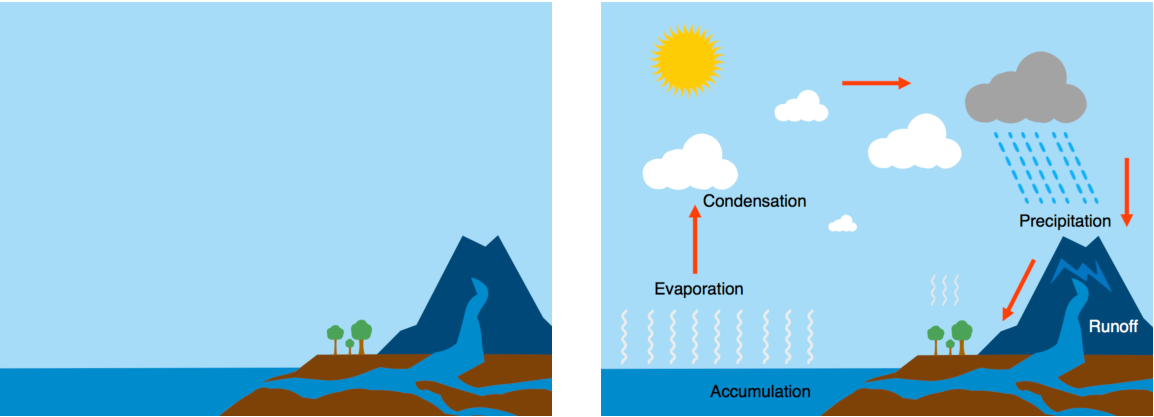
\includegraphics[width=2.0\columnwidth]{figures/watercycle}
%  \caption{}~\label{fig:watercycle}
%\end{figure*}
\subsection{Slide authoring}
Slides in Aparecium can be authored using any existing slide presentation software (e.g., PowerPoint, Keynote, GoogleSlides). They can include typed text or images, as well as, hand drawn ink strokes. Instead of specifying animation effects on these slide elements, presenters separate them into two layers for each slide. The background layer is always visible and it is what the audience sees initially. The foreground layer is initially only visible on the presenter view, but presenters can reveal parts of it to the audience during delivery. Presenters also have the option of preparing a third layer, the notes layer, which is only visible on the presenter view and acts as transparent speaker notes placed on top of the slides. Layers in Aparecium are represented as bitmap images. (Figure~\ref{fig:slidelayers})

\begin{figure*}[h!]
    \centering
    \begin{subfigure}[t]{0.31\textwidth}
        \centering
        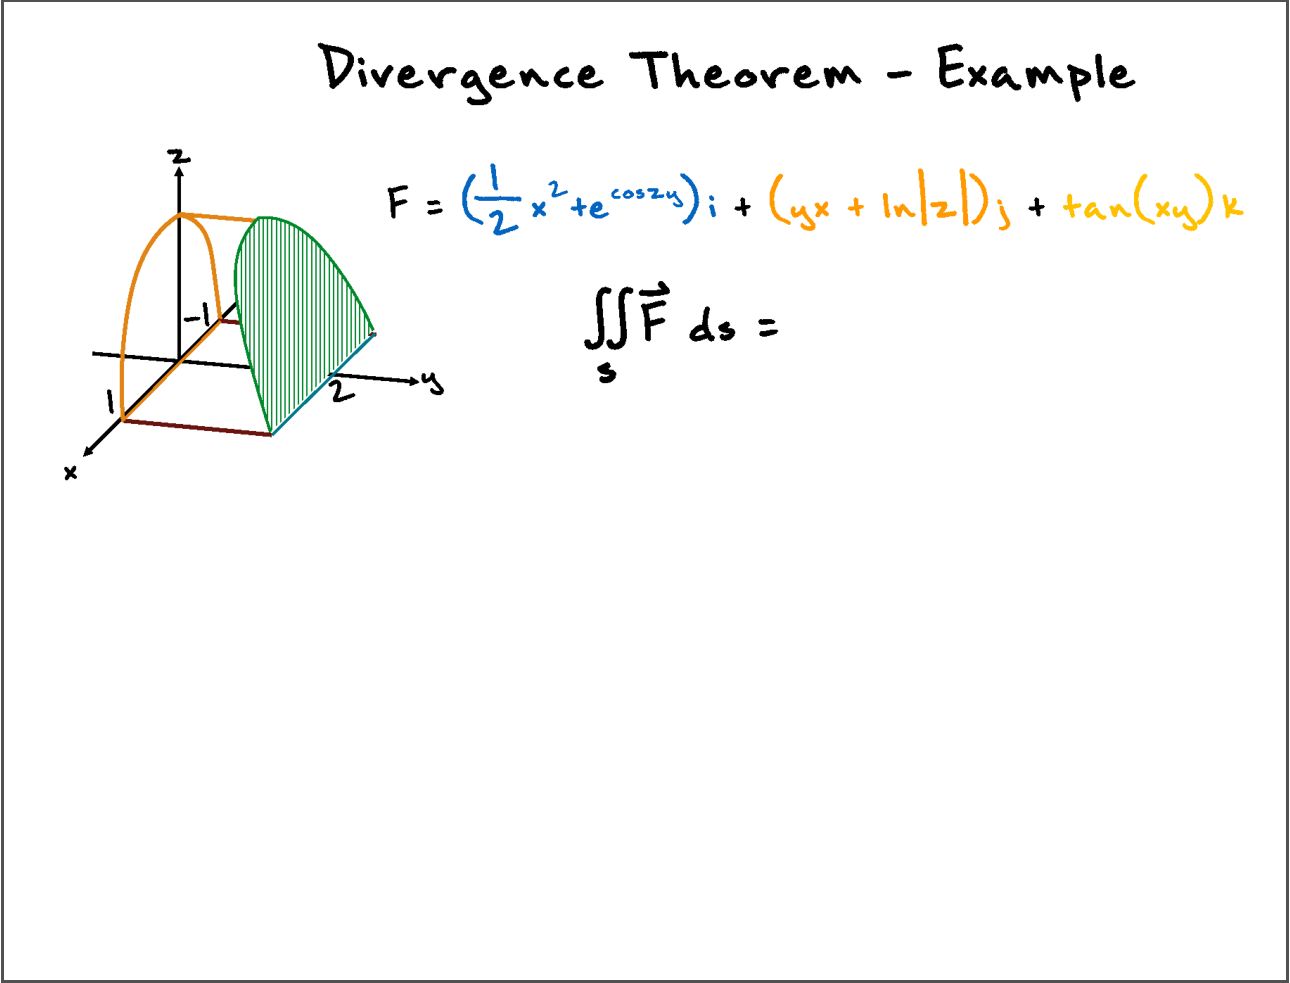
\includegraphics[width=1\columnwidth]{figures/videoslide1}
\captionsetup{font=footnotesize}
        \caption{Background (Audience View)}
    \end{subfigure}%
    ~ 
    \begin{subfigure}[t]{0.31\textwidth}
        \centering
        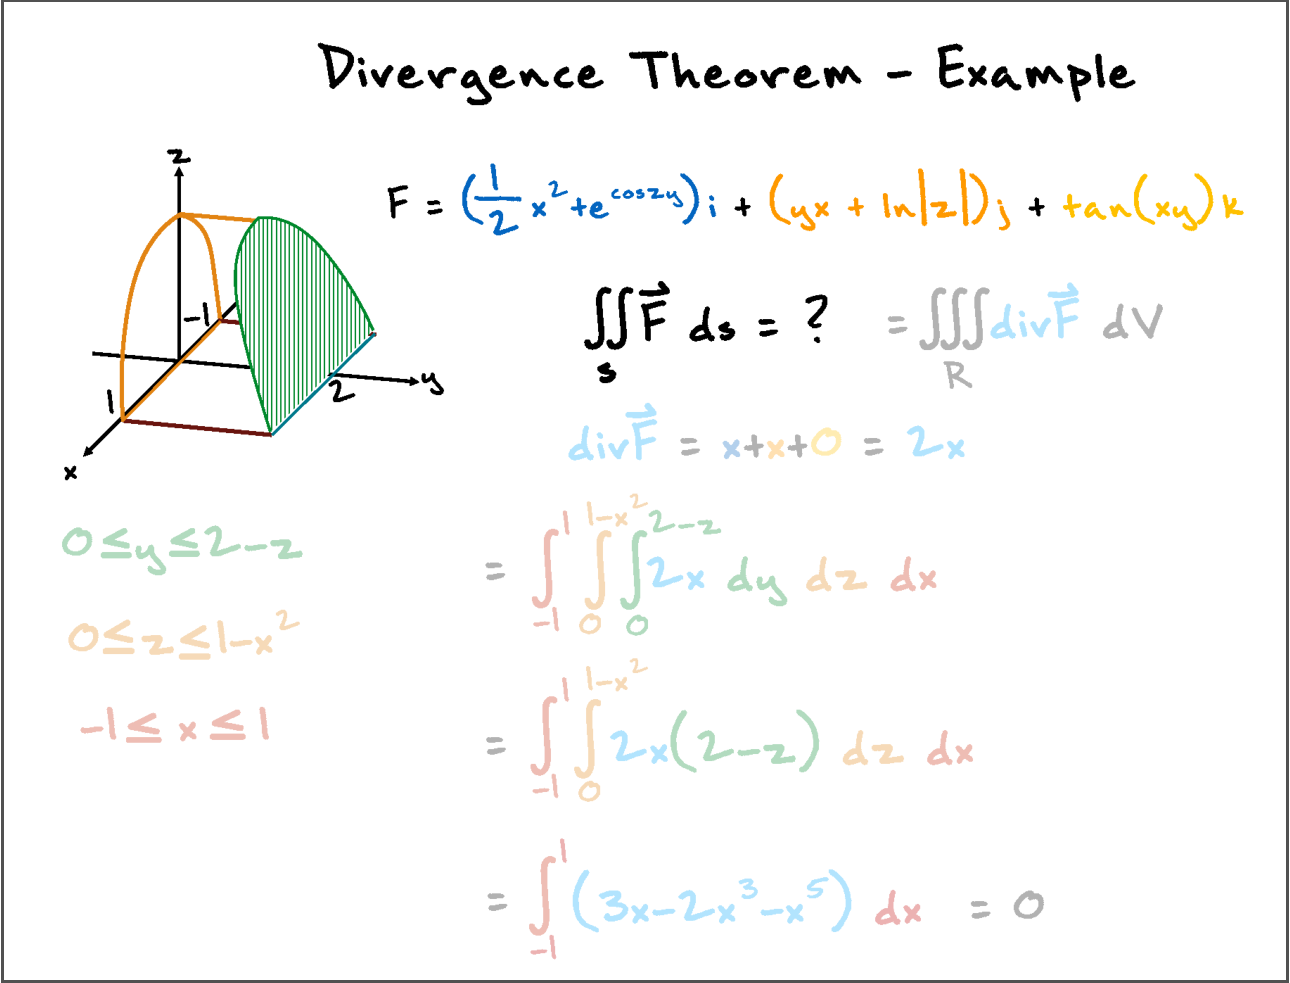
\includegraphics[width=1\columnwidth]{figures/videoslide2}
        \captionsetup{font=footnotesize}
        \caption{Background + Foreground\\ (Presenter View)}
    \end{subfigure}
    ~
        \begin{subfigure}[t]{0.31\textwidth}
        \centering
        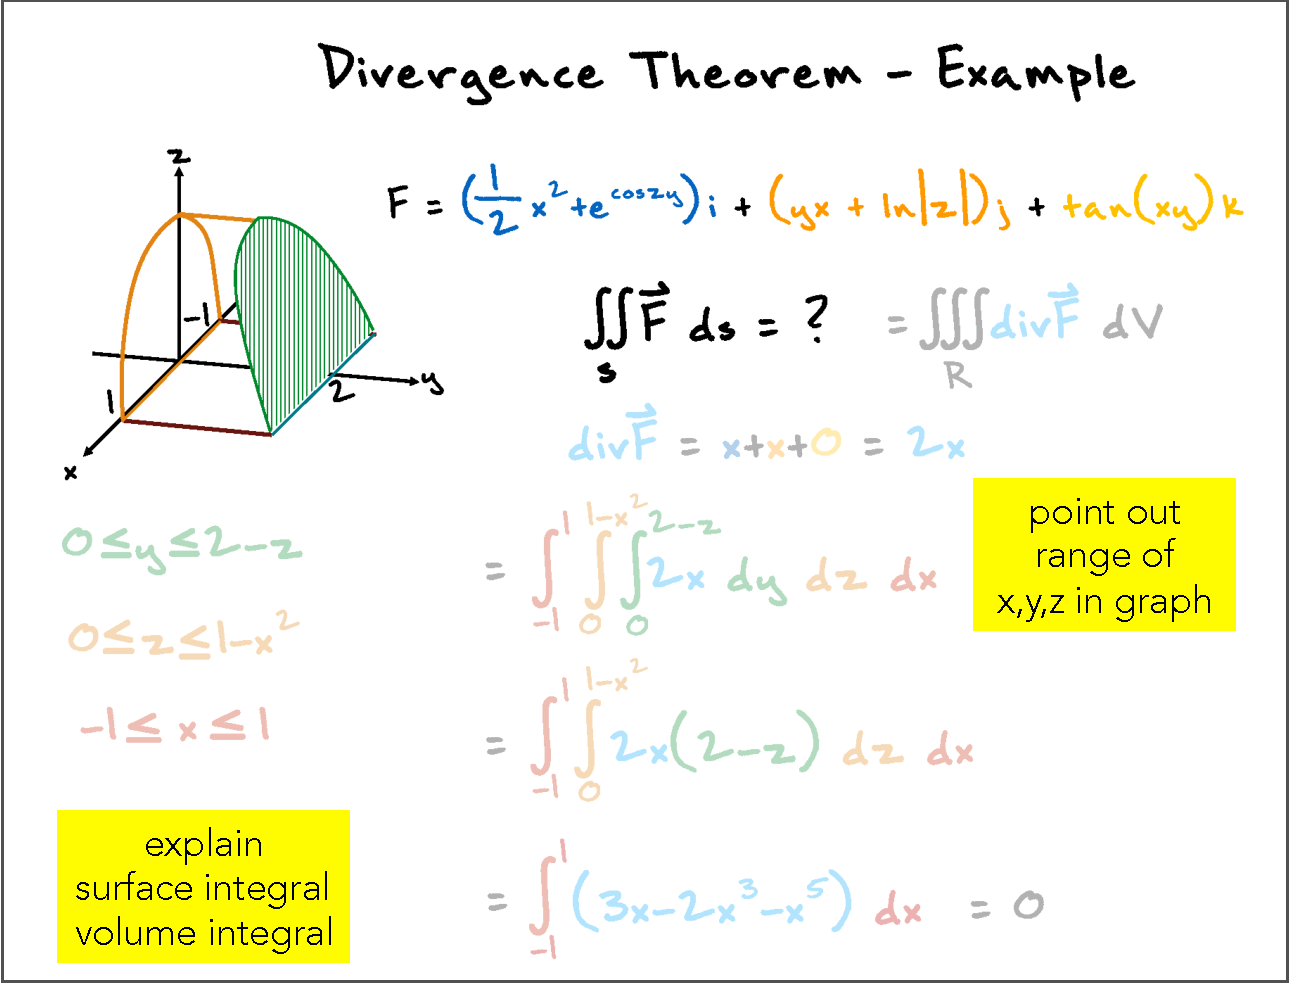
\includegraphics[width=1\columnwidth]{figures/videoslide3}
        \captionsetup{font=footnotesize}
        \caption{Background + Foreground + Notes}
    \end{subfigure}
    \caption{Slide Layers in Aparecium. Slides are separated into foreground and background layers. \textbf{(a)} The background layer is always visible and it is what the audience sees initially. \textbf{(b)} The foreground layer is initially only visible on the presenter view, and is faded to distinguish it from the background. Presenters can reveal parts of it to the audience during delivery. The revealed parts appear on the audience view and becomes unfaded on the presenter view. \textbf{(c)} Optionally, presenters can also have the notes layer, which is only visible on the presenter view and acts as transparent speaker notes placed on top of the slides. }
    \label{fig:slidelayers}
\end{figure*}

\subsection{Inking during delivery}
%
Aparecium enables robust, modeless inking operations at presentation time by leveraging the structure of the pre-authored slide content. Each of the three inking functions uses this structure in different ways. 
\subsubsection{Reveal}
To reveal hidden foreground content to the audience, the presenter inks over the relevant portion of the foreground layer.
%
At the end of each stroke, the system computes a subset of the surrounding foreground pixels to display. 
%
For each point, $s_i$ on the stroke, the closest foreground pixel, $p_i$ is computed. If the distance between $p_i$ and $s_i$ is within a threshold $\alpha$, a flood-fill is performed starting from $p_i$ to neighboring foreground pixels. The value of $\alpha$ determines how precisely the user has to ink in order to reveal the underlying content. Since presenters can be more precise when they are inking slowly versus when they are inking quickly, $\alpha$ is set to vary proportionally to inking velocity, $v$:
%
\begin{equation}
\alpha = 0.02v+10
\end{equation}
where both $\alpha$ and $v$ are measured pixel space.\\
 
The extent of the flood-fill is limited by two additional thresholds $\beta$ and $\gamma$ on (1) the distance from $p_i$, and (2) the color difference from $p_i$ in Lab space. 
%
To give presenters finer-grained control over the extent of the reveal, $\beta$ and $\gamma$ also vary according to the velocity of the presenter's ink stroke:\\ 
\begin{equation}
    \beta = min(0.01v+5,\;40)
\end{equation}
%
\begin{equation}
\gamma = 0.05v+10
\end{equation}

Our algorithm has several important properties. Bounding the flood-fill with $\beta$ and $\gamma$ ensures that the revealed content is localized around the user stroke and prevents ``bleeding'' across regions with very different colors.
%
In addition, modulating $\beta$ and $\gamma$ based on the stroke velocity allows presenters to reveal with different levels of precision. 
%
To show a small piece of content, the presenter can ink slowly over the relevant foreground region. This interaction is useful when the presenter wants to simulate writing in real-time, or needs to reveal a specific element in a dense slide. For example, in Figure~\ref{fig:inkreveal}(a), the presenter slowly writes out a part of the integral $\int_{-1}^{1}\int_{0}^{1-x^2}\int_{0}^{2-z}2x$, while explaining each of the domains.
%
In other situations, users may want to reveal larger pieces of content more efficiently. For example, in Figure~\ref{fig:inkreveal}(c), the presenter reveals all of $dxdydz$ at once to complete the equation. In this case, users can ink quickly and roughly (e.g., by scribbling) over a foreground region.

\begin{figure}[h!]
    \centering
    \begin{subfigure}[t]{0.4\columnwidth}
        \centering
        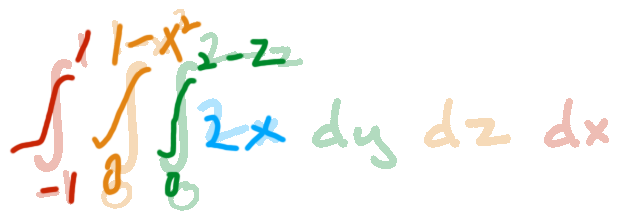
\includegraphics[width=1\columnwidth]{figures/slowink_presenter}
                \captionsetup{font=footnotesize}
\caption{Slowly writing over a portion of the equation (Presenter View)}
    \end{subfigure}%
    ~ ~
    \begin{subfigure}[t]{0.4\columnwidth}
        \centering
        
\includegraphics[width=1\columnwidth]{figures/slowink_audience}
                \captionsetup{font=footnotesize}
\caption{After reveal \\ (Audience View)}
    \end{subfigure}
         ~   ~
      \begin{subfigure}[t]{0.4\columnwidth}
        \centering
        
\includegraphics[width=1\columnwidth]{figures/fastink_presenter}
                \captionsetup{font=footnotesize}
\caption{Quickly scribbling over rest of the content (Presenter View)}
    \end{subfigure}%
    ~ ~
    \begin{subfigure}[t]{0.4\columnwidth}
        \centering
        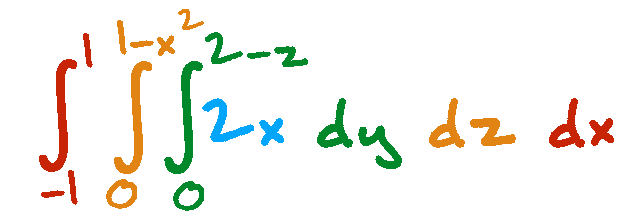
\includegraphics[width=1\columnwidth]{figures/fastink_audience}
                \captionsetup{font=footnotesize}
\caption{After reveal (Audience View)}
    \end{subfigure}
    \caption{Inking to reveal. Presenter inks over foreground content to reveal it to the audience. Presenter can either \textbf{(a)} ink over slowly to simulate writing in real-time, or \textbf{(b)} scribble over quickly to reveal larger portions efficiently. \textbf{(c), (d)} In both cases, the relevant portion of the foreground layer is revealed to the audience and replaces the presenter's original ink strokes.}
    \label{fig:inkreveal}
\end{figure}

\subsubsection{Annotate}
Presenters sometimes add new (i.e., unauthored) information to a slide on-the-fly during a presentation.
%
For example, a lecturer may circle an important concept for emphasis, explicitly label part of a diagram, or even add a whole new line of equation. 
%
To make such annotations in Aparecium, the presenter simply inks over empty (or already revealed) pixels on the foreground layer. If less than 10\% of the $p_i$s are within the $\alpha$ threshold of an unrevealed foreground pixel, the system treats the stroke as an annotation. To ensure that the annotation stands out from the surrounding slide content, Aparecium computes the average color of the slide around the stroke and sets the ink to a complementary color. (Figures~\ref{fig:annotate} and \ref{fig:space}c). 

\begin{figure}[h!]
    \centering
    \begin{subfigure}[t]{0.5\columnwidth}
        \centering
        
\includegraphics[width=1\columnwidth]{figures/annotate_presenter}
                        \captionsetup{font=footnotesize}
        \caption{Before auto-coloring}
    \end{subfigure}%
    ~ 
    \begin{subfigure}[t]{0.5\columnwidth}
        \centering
        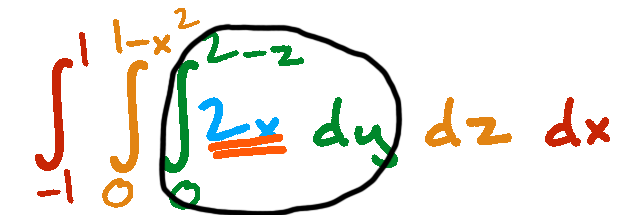
\includegraphics[width=1\columnwidth]{figures/annotate_audience}
                        \captionsetup{font=footnotesize}
\caption{After auto-coloring}
    \end{subfigure}
    \caption{Inking to annotate. \textbf{(a)} Presenter inks over already revealed content to make annotations. \textbf{(b)} To ensure that the annotation stands out from the surrounding slide content, Aparecium computes the average color of the slide around the stroke and sets the ink to a complementary color. In this case, the underlines below the cyan $2x$ is set to orange.}
    \label{fig:annotate}
\end{figure}

\subsubsection{Create Space}
In some cases, presenters may want extra space to insert new content in a slide, for example, to add an item to an existing list, a word in a sentence, or an extra line of explanation. These situations can arise as a result of a mistake in the preparation phase (e.g., the presenter forgets to list an item), as well as from presenter-audience interaction (e.g., the audience requests extra explanation). Aparecium allows presenters to create empty space from ink strokes. First, the presenter draws a curve where the empty space should be created. At the end of the curve, if the presenter holds down the pen for more than 0.5 seconds, the curve turns into a red dashed stroke, indicating that the presenter can start expanding the space around the curve. As the presenter moves the pen along one of the axis-aligned directions, empty space is created and expanded from the curve in that direction.  As the space grows, the foreground content shifts accordingly. (Figure~\ref{fig:space}).

%
\begin{figure}[h!]
    \centering
    \begin{subfigure}[t]{0.48\columnwidth}
        \centering
        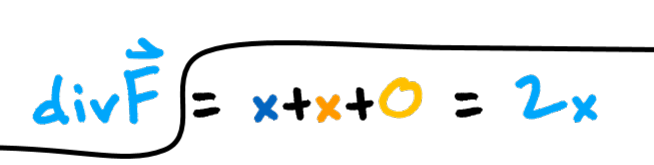
\includegraphics[width=1\columnwidth]{figures/create_space1}
                       \captionsetup{font=footnotesize}
 \caption{Presenter draws a stroke where empty space should be created and holds the pen down (0.5sec)}
    \end{subfigure}%
    ~ 
    \begin{subfigure}[t]{0.48\columnwidth}
        \centering
        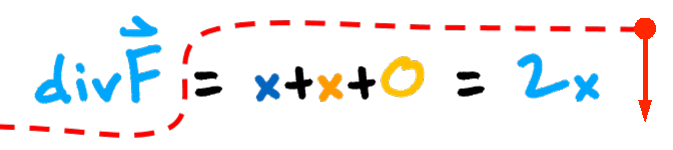
\includegraphics[width=1\columnwidth]{figures/create_space2}
                       \captionsetup{font=footnotesize}
 \caption{The stroke turns into a space-expansion curve. Empty space is created by expanding the curve along the direction of the pen movement and shifting the foreground content accordingly.}
    \end{subfigure}
    ~
        \begin{subfigure}[t]{1\columnwidth}
        \centering
        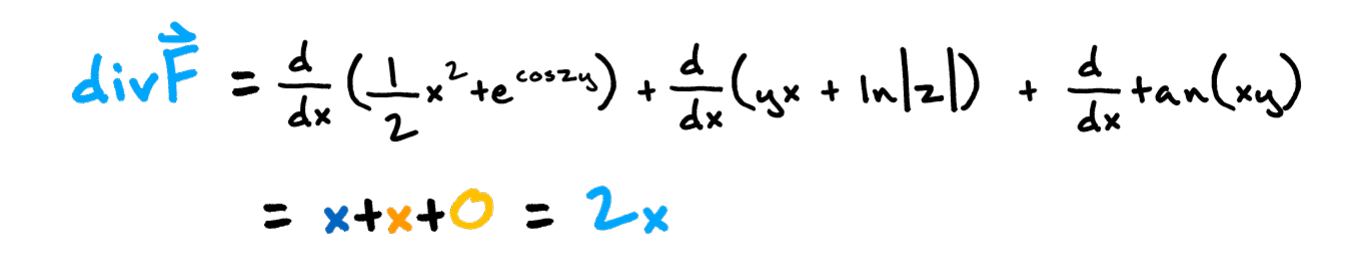
\includegraphics[width=1\columnwidth]{figures/create_space3}
                        \captionsetup{font=footnotesize}
\caption{Presenter inserts annotations in the newly created space }
    \end{subfigure}  
    \caption{Creating space and annotating.}
    \label{fig:space}
\end{figure}
%
As space is created, the slide area grows and scrolling is automatically enabled. Users can also zoom out to fit the slide in a single view.
%----------------------------------------------------------------------------------------

\section{User Evaluation}

We evaluate Aparecium from the perspective of presenters and the audience. We assess the ease of use of the interface from the presenters' point of view, and rate the presentation quality from both the presenters' and the audiences' perspective.\\

To better understand the benefits of our interface, we compared Aparecium against two baselines. The first baseline (\textbf{BaselinePPT}) represents conventional electronic slide tools.
%
We use Microsoft PowerPoint and allow presenters to apply animation effects (but no inking) during the presentation.
%
The second baseline (\textbf{BaselineInk}) represents standard ``blackboard-style'' presentation tools that allows users to ink in real-time during the presentation.
%
For this condition, we also use Microsoft PowerPoint but only allow users to pre-author and deliver content via inking.\\

We hypothesized that different types of content would lend themselves to different presentation styles. We compare three different types of content: (1) a text-centered slide, explaining the derivation of the quadratic formula \textit{(Derivation)}, (2) a diagram-centered slide, describing the hydrologic cycle  \textit{(WaterDiagram)}, and (3) a typical PPT style slide with bullet points and images listing different carpentry tools \textit{(BulletPoints)}. Using PowerPoint, we pre-authored a single page slide for each of these content types (Figure~\ref{fig:studyslides}).\\
%
\begin{figure}[h!]
    \centering
    \begin{subfigure}[t]{1\columnwidth}
        \centering
        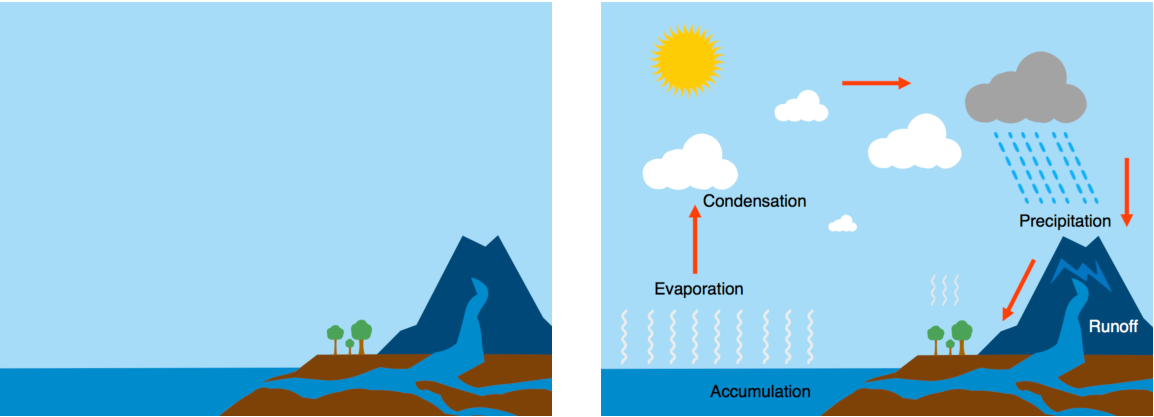
\includegraphics[width=1\columnwidth]{figures/watercycle}
        \captionsetup{font=footnotesize}\caption{\textit{WaterCycle} slide background (left) and foreground (right)}
    \end{subfigure}
    ~ 
    \begin{subfigure}[t]{0.48\columnwidth}
        \centering
        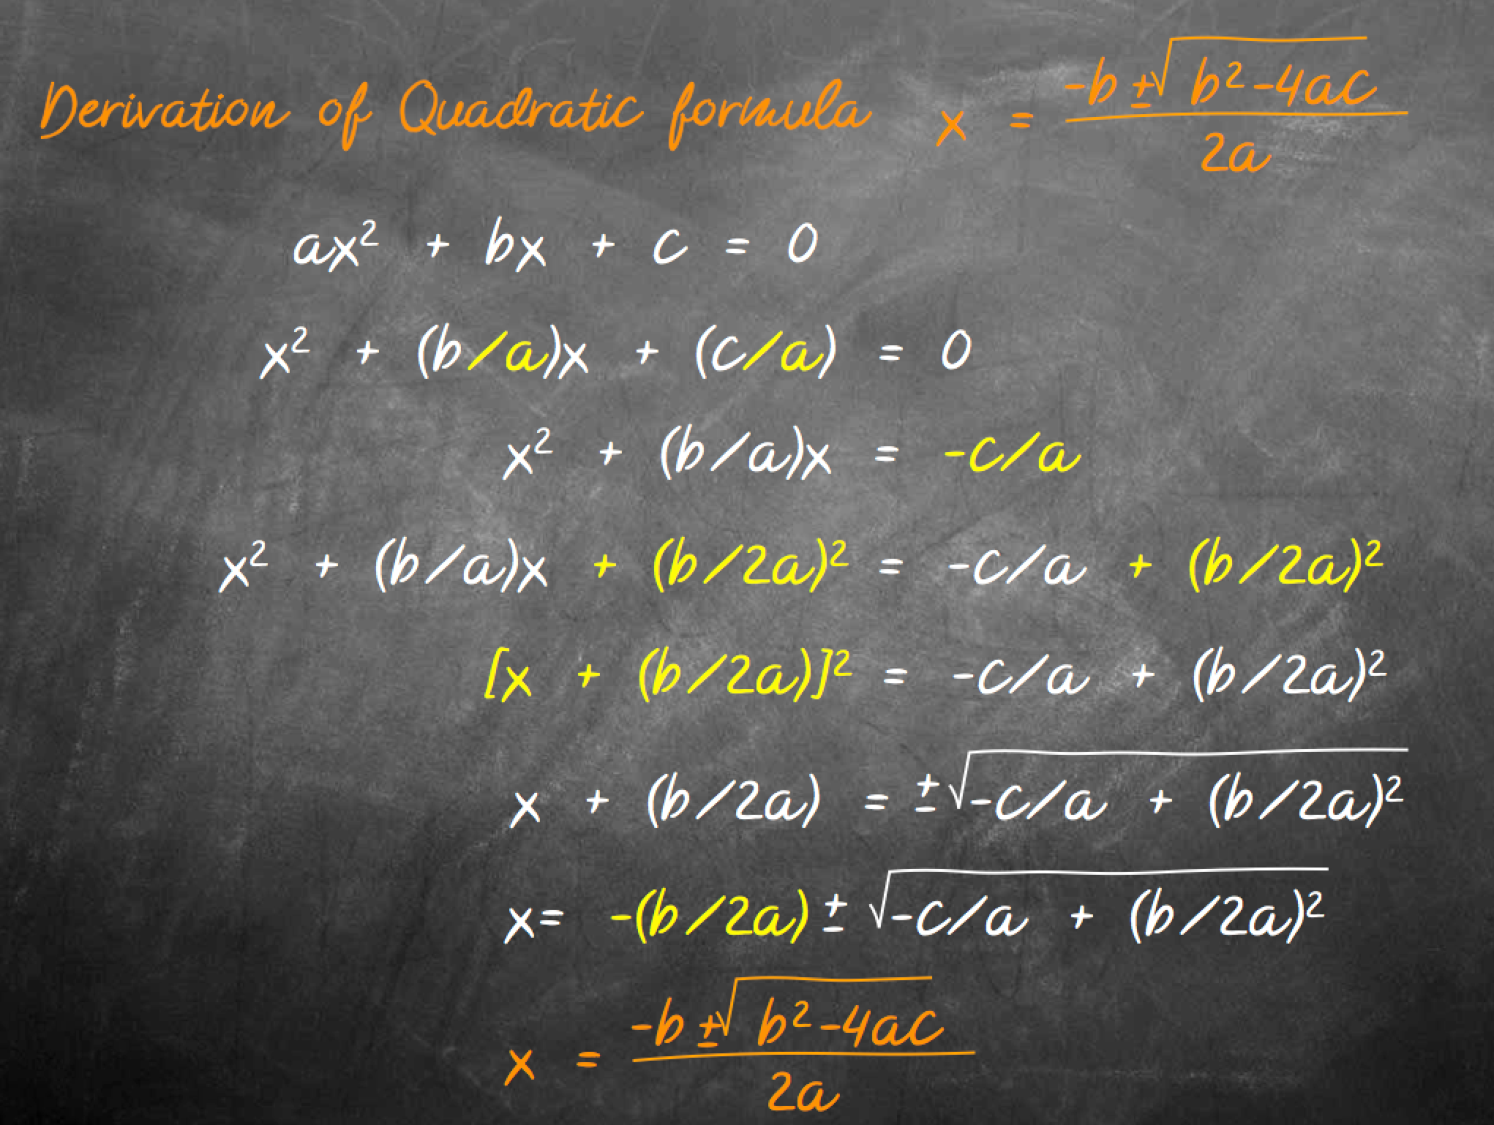
\includegraphics[width=1\columnwidth]{figures/quadformula}
        \captionsetup{font=footnotesize}\caption{\textit{Derivation} slide}
    \end{subfigure}  
    ~
    \begin{subfigure}[t]{0.48\columnwidth}
        \centering
        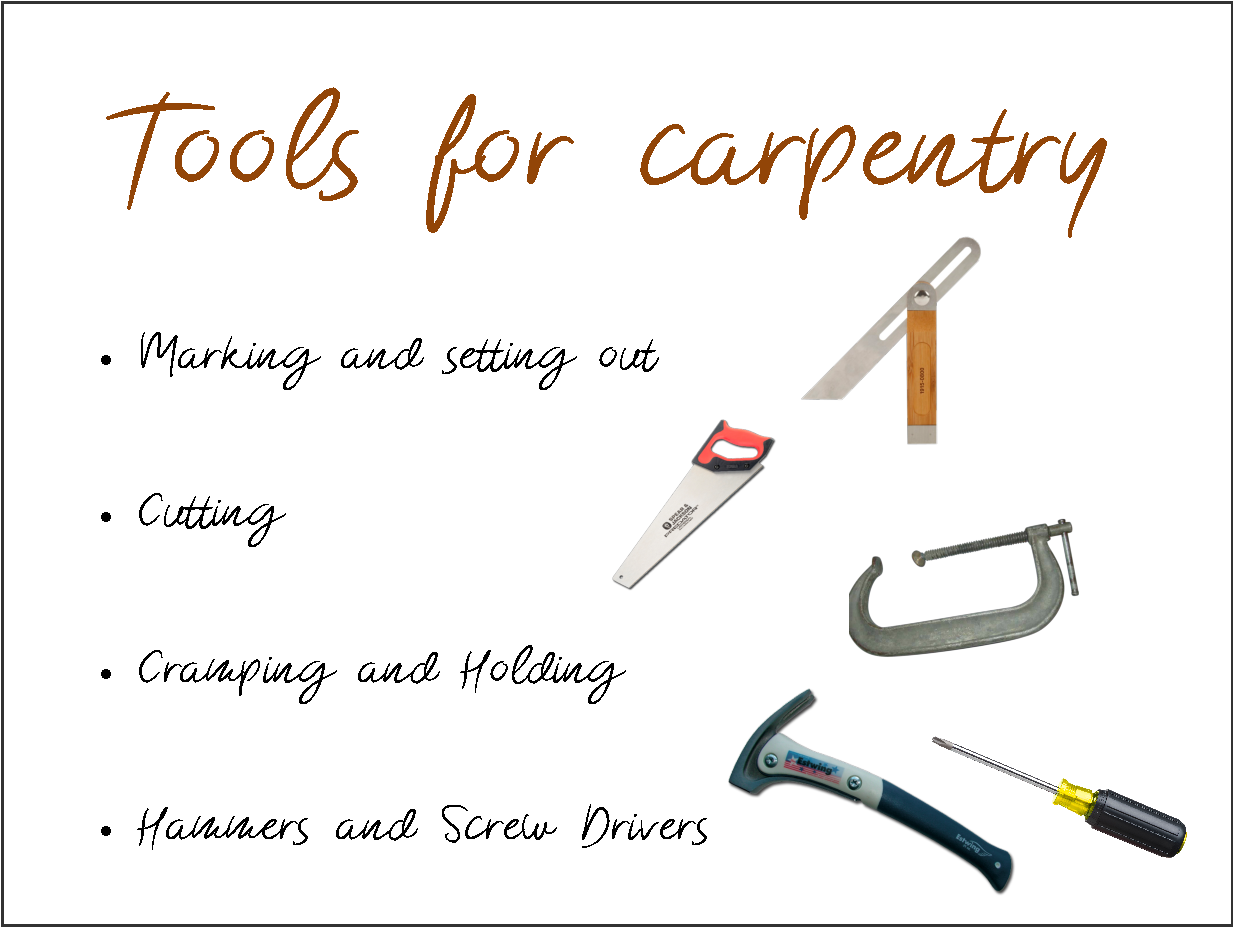
\includegraphics[width=1\columnwidth]{figures/tools}
        \captionsetup{font=footnotesize}\caption{\textit{BulletPoints} slide}
    \end{subfigure}  
    \caption{Evaluation slides}
    \label{fig:studyslides}
\end{figure}

To reduce the preparation effort for all three presentation tool conditions, we separated each slide into foreground and background elements, which are shown in our supplemental materials. For the BaselinePPT condition, we leave the individual PowerPoint elements (e.g., arrows, text boxes containing individual lines of equations, images) ungrouped to make it easier for users to author fine-grained animations. 

\subsection{Study 1: Presenter Perspective}
In our first study, we asked participants to present each of the three content types using the three different presentation tool conditions. 
%
For each content type, participants were given the pre-authored, pre-segmented slide. 
They received verbal and written explanations of the material, and a printout of the complete slide contents (both foreground and background layers). They were given time to familiarize themselves with this material and to set up the slide before the presentation.\\

In the BaselinePPT condition, participants could add animation effects to reveal or emphasize the foreground elements. For the BaselineInk condition, the slide only contained background elements. Participants were free to write additional content into the slide as part of their set up, which is analogous to blackboard lecturers writing on the board before class. For Aparecium, participants could also write additional content on top of the background, or they could choose to make some of the foreground elements visible (effectively moving those elements into the background layer). For simplicity, we omitted the space creating functionality in the evaluation. \\

After the setup phase, participants used one of the three tool conditions to deliver the presentation. 
%
To simulate a real presentation, participants were asked to pretend that their presentation was being broadcast live as a webcast. At the end of each trial, we showed the user a screen recording of their presentation and asked them to self-rate their own presentation, this time pretending that they were students trying to learn the subject. Presenters also completed a questionnaire where they rated how easy it was to prepare and deliver presentations using each of the tools. All ratings were done on a 5-point Likert scale.\\

We recruited 12 graduate students from 8 different universities (ages 21 to 31). All of the partcipants were familiar with the PowerPoint interface. We used a within-subject design, where each participant delivered presentations on each interface. We kept the task order fixed and counter-balanced the order of the presentation tools to obtain an equal distribution of task-tool pairs.
%

\subsection{Study 2: Audience Perspective}
In our second study, we recruited a separate set of participants to vote on presentations delivered using each interface.
%
While we considered comparing the output presentations from the first study, we found that there was too much variation in quality between the results. Since presenters were not forced to follow fixed scripts, there were significant differences in length and detail. In addition, the presenters spoke with varying levels of enunciation and enthusiasm (not to mention different accents).
%
Thus, we ourselves produced a new set of more comparable presentations
using the slides from the first study.
%
To make the comparison as fair as possible, we used a fixed script for each content type.
We also analyzed the output presentations from the first study, and used them as a reference when creating our own versions. 
%
For example, for the BaselinePPT condition, we reproduced the granularity and order of animations that we observed in the user-created presentations.
%a
In the BaselineInk condition, we followed the typical ordering of the inked contents and chose similar ink colors. We also recorded the presentations so that the silent pauses in between inking periods were similar (or shorter) than those produced in the first study. 
%
Finally, for Aparecium, we used a similar reveal order, combination of slow tracing versus fast scribbling, and on-the-fly ink annotations as most participants. 
%
In general, presenters from the first study employed similar approaches to inking or animation so it was straightforward to extract common qualities. For the few cases, where participants varied in their approach, we selected an approach that we deemed to produce better quality (e.g., finer-grained animations, use of different ink colors).\\
 
We recruited 36 undergraduate and graduate students from multiple universities to rate the presentations. For each content type, participants watched recordings of three presentations delivered using each interface, and voted for the most engaging presentation. 

\subsection{Findings and Discussion}
Overall, presenters found Aparecium easy to use for setting up and delivering presentations. They were satisfied with the quality of the presentations recorded using our interface, and emphasized that the appearance of real time inking had an engaging effect. 
Preferences between the presentation tools depended on the content type. Participants in both studies (i.e., presenters and viewers) preferred Aparecium for text-centered or process-driven content. \\

Given the size and exploratory nature of our study, we use descriptive statistics to summarize the Likert responses from Study 1. Below we discuss each of our findings in more detail.\\

\subsubsection{Aparecium makes it easier to prepare slides.}
Presenters found it easiest to set up the slides using our interface, followed by BaselineInk and then BaselinePPT (Figure~\ref{fig:likert}). 
%
\begin{figure}[h!]
    \centering
        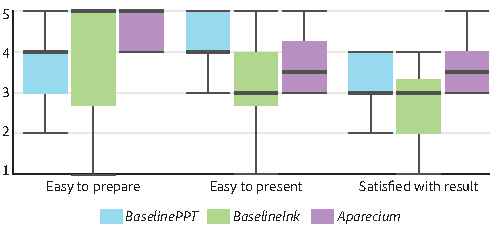
\includegraphics[width=0.8\textwidth]{figures/study1likert}
        \caption{Summary of Likert responses from Study 1 on a scale from 1 (strongly disagree) to 5 (strongly agree).}
\label{fig:likert}
\end{figure}
%
With Aparecium, most presenters did not do any extra work (revealing or writing beforehand) to set up the slides, but used them as-is. In the few cases, where they pre-revealed parts of the foreground, they expressed that the required effort was minimal.\\ 

In comparison, although our participants were familiar users of PowerPoint, they found the effort to set up animation effects tedious. To quote \textit{U6}, "\textit{It was cumbersome to add animations to each individual object and get the timing right... sometimes I decided I wanted to add an animation, but then had to figure out where to insert it in the existing animations sequence.}"\\

In terms of preparation effort, the BaselineInk condition was similar to our interface; most participants used the slide as-is, without writing additional content ahead of time. However, the reasons were different. In Aparecium, presenters had the ability to reveal the pre-authored foreground elements to the audience during the presentation. In the BaselineInk condition, presenters had to manually draw the foreground content, which they could either do ahead of time (thus losing the real-time effect) or during delivery. Either way, the effort was more \textit{"daunting"  (U12)} and  \textit{"time consuming" (U8)}, and the result was aesthetically less satisfactory (\textit{U1, U5, U8}).  
%%\val{Kruskall-Walis: chi-squared; 4.865, p = 0.0878}

\subsubsection{For presentation delivery, Aparecium involves comparable effort to BaselinePPT and less effort than BaselineInk.}
%{Kruskall-Walis chi squared: 4.044, p = 0.13}
%Presenters found it easiest to deliver the presentation using BaselinePPT, followed by our interface, and then BaselineInk.The difference between BaselinePPT and our interface (Mann-Whitney U test: Z = 1.18, p = .24) was less significant than between that of BaselinePPT and BaselineInk (Z = -1.88, p = .06). \\
%
Regarding the ease of delivering presentations, BaselinePPT received slightly higher ratings than our interface. BaselineInk was rated the lowest by a larger margin. 
%
It is not surprising that BaselinePPT required the least effort. The only interaction presenters used was to press a single button to advance the slide animations. That said, when the animation involved more than a few steps, it was common for presenters to make mistakes. 3 out of 12 participants forgot to advance the animation at the right time at least once, and only realized it at the next animation step. They had to either repeat the verbal explanation or quickly skip through the subsequent animations. In addition, two participants reported that they forgot to set up a desired animation step and only realized it during delivery. Several users suggested that having cues to help remember the animation would be beneficial $(U2, U7)$.\\

While presenters found inking in Aparecium straightforward, they noted that inking to reveal still required more effort than pushing a single button. Presenters seemed to prefer the path of minimum effort. For instance, with the exception of the math derivation content, they mostly used fast scribbling or strike-through gestures to reveal. As several presenters mentioned, this had the downside that the audience would initially see the scribbled ink strokes before the underlying pixels were revealed, which could potentially be distracting and aesthetically less pleasing. Some users suggested that they would prefer an even faster gesture such as clicking or circling to reveal large parts. On the other hand, they also expressed the idea that for the audience it could be better \textit{"to have the word appear after the inking instead of just after clicking like in powerpoint." (U1)} We discuss this tradeoff in more detail in the Limitations and Discussion section. In addition, users appreciated the automatic color selection for annotation and the modeless switching between revealing and inking. \\

As expected, BaselineInk required the most effort during delivery. Participants complained that drawing took away their attention from the content delivery. Since verbal explanations tend to be faster, there were periods of silence while the presenters were still drawing. In the Derivation presentation, three out of the four presenters who used BaselineInk ran out of space and had to use the margins or eraser. The one exception was a presenter who used the setup time to layout line numbers on the slide. In addition to these challenges, some users also complained about the specific difficulty of writing on a tablet. For example, the screen interface is not as smooth as paper \textit{(U1, U4, U6)} and operations such as switching to an eraser or a different color is tedious \textit{(U7, U9)}. 

\subsubsection{Presenters were most satisfied with the presentation quality of Aparecium.}
Presenters were most satisfied with the presentations produced using Aparecium. As shown in Figure~\ref{fig:likert}, the distribution of ratings for BaselinePPT was slightly lower, while BaselineInk was rated the lowest.
%
%The difference between our interface and BaselinePPT was less significant (Z = -0.95, p = .34) than that between ours and BaselineInk (Z = -1.88, p = 0.06). 
%
This trend held overall, as well as for each individual content type.\\

The feedback we gathered was consistent with our preliminary, formative interviews. Participants were accustomed to the BaselinePPT style, but in many cases they thought it could be improved with finer grained animation \textit{(U1, U3, U4, U8, U11)}. They liked the \textit{"handwritten in real time effect" (U4)}   in Aparecium, as it made the presentation \textit{"more interactive and seem to require engagement " (U9)}. The main complaints about BaselineInk presentations were that the drawings looked \textit{"messy" (U7)} and \textit{"not professional enough" (U6)}, and that the pace was too slow.\\

\subsubsection{Tool preference depends on presentation content.}
Figure~\ref{fig:votes} shows the preference data across content types from both studies. The tool preferences of both the presenters and audience depended on the content type.\\
%
\begin{figure}[h!]
    \centering
        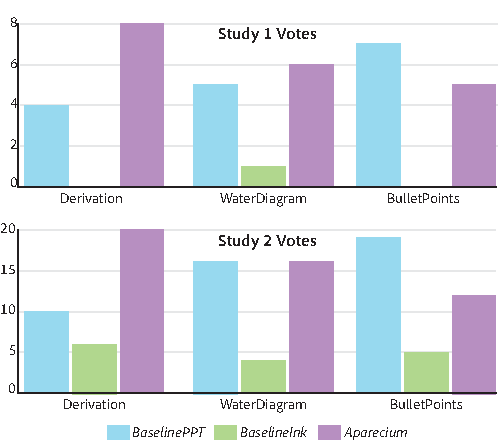
\includegraphics[width=0.8\textwidth]{figures/studyVotes}
        \caption{Preferred tool/presentation for each content type.}
\label{fig:votes}
\end{figure}
%

In Study 1, we asked presenters to choose which interface they would prefer to use for each content type.
For Derivation, presenters preferred  Aparecium (8/12) and then BaselineInk (4/12). For WaterDiagram, Aparecium (6/12) and BaselinePPT(5/12) were comparable choices. Similarly for BulletPoints, BaselinePPT (7/12) and Aparecium (5/12) were preferred.\\
%

In Study 2, we asked audiences which presentation was most engaging. For Derivation, the majority of audiences preferred Aparecium (20/36) followed by BaselinePPT (10/36) and then BaselineInk (6/36). For WaterDiagram, Aparecium (16/36) and BaselinePPT (16/36) were comparable. For BulletPoints audiences preferred BaselinePPT (19/36) and then Aparecium (12/36).\\

These findings confirm our intuition that fine-grained control of pace is most important for presenting sequential processes, especially for writing out text or equations (Derivation). In the case of the WaterDiagram, it was easy to achieve similar sized steps using BaselinePPT and Aparecium. The fact that the WaterDiagram slide consists mainly of images rather than text may have affected the users choice as well (see discussion about different ways to reveal). For simple lists and images (BulletPoint), BaselinePPT provided an appropriate pace and aesthetics.

%----------------------------------------------------------------------------------------

\section{Discussion}
Here, we consider some limitations of our design, and discuss several observations and lessons learned about designing future presentation interfaces.

\subsection{Limitations}
\subsubsection{Different Ways to Reveal.}  
Several presenters in the first user study wanted an even quicker way than scribbling to reveal content. Indeed, scribbling over large areas to reveal images or long lines of text can be tedious, especially if the presenter is not concerned about simulating the real-time hand-drawn effect. \\

In addition, some participants across both user studies complained that showing the scribbles before revealing the foreground elements is less aesthetically pleasing or even distracting. Conversely, other audience members commented that the scribbles served as helpful cues to draw attention to where information was about to appear.\\

In general, supporting different types of revealing mechanisms (e.g., clicking or lasso selection) and allowing instantaneous reveal of certain elements could improve the presentation experience. However, such a design should not increase the preparation effort or limit flexibility during presentation. For example, we considered allowing presenters to specify at setup time elements that can be revealed instantaneously upon clicking or tapping. However, this can make preparation tedious, akin to grouping elements and setting up animations in PowerPoint. Moreover, it does not allow presenters to change their mind during preparation about how to reveal elements. 

\subsubsection{Presenter Convenience vs. Presentation Quality.} 
The question of what revealing mechanisms to support points to a more fundamental tension with presenter interfaces. On the one hand, making the workflow more convenient for presenters is an important objective. However, it is at least as important to take into account the audience's point of view, since they are the intended consumers of the presentations themselves. For example, providing a larger set of revealing gestures may tempt presenters to always opt for the minimum-effort gesture at the cost of presentation quality. In fact, in an earlier prototype of our system, we allowed revealing either by lasso selection or slow tracing, and observed that presenters almost always opted for the lasso tool even for the \textit{Derivation} type of content, which compromised presentation quality for the audience. Instead, we opted for a design that \textit{forces} the presenter to go at a slower pace.\\

More broadly, designing presentation tools that achieve the right balance between the needs of presenters and audience members remains an interesting direction for future work. In this vein, previous research that systematically compares the effect of different presentation styles (e.g.,~\cite{seth2010powerpoint, cross2013typerighting}) may provide valuable guidance for new interfaces that assist and \emph{nudge} presenters towards the most effective communication techniques.

\subsubsection{Creating Flexible Interactivity.} 
Our work focuses on presenting slides with static visuals, and Aparecium supports limited interaction with the displayed content (i.e., shifting elements to create empty space). In our formative interviews, several participants expressed the desire to present interactive content that can be controlled on-the-fly, for instance, to explain the steps of a computer algorithm or a physics diagram. 
%
While there are many existing approaches to creating interactive diagrams, designing authoring and presentation tools that are both convenient and flexible is a challenging problem that bears further exploration.

\subsection{Conclusion}
This chapter introduced Aparecium, a novel presentation interface that combines inking interactions with pre-authored slides to help presenters deliver flexible and engaging presentations.\\

Our modeless inking interactions allow presenters to reveal, annotate and create extra space during a presentation. We evaluated our interface from the perspective of presenters and the audience by comparing it against two baseline interfaces, representing conventional slide and inking tools. Presenters found our interface easy to use both during preparation and delivery. In particular, for text-heavy, process-driven content, both presenters and audience preferred presentations delivered using Aparecium.\\ 

In light of these findings, we believe our inking interactions could be a valuable addition to existing slide-based presentation tools.


 % Chapter 4 
%\cleardoublepage
%% Chapter 4

\chapter{Conclusion} % Chapter title

\label{ch:conclusion} % For referencing the chapter elsewhere, use \autoref{ch:name} 

%----------------------------------------------------------------------------------------

\section{Section Title}

Content

%------------------------------------------------

\subsection{Subsection Title}

Content

%------------------------------------------------

\subsection{Subsection Title}

Content

%----------------------------------------------------------------------------------------

\section{Section Title}

Content % Chapter 4 


%\cleardoublepage % Empty page before the start of the next part

%----------------------------------------------------------------------------------------
%	THESIS CONTENT - APPENDICES
%----------------------------------------------------------------------------------------

%\appendix

%\part{Appendix} % New part of the thesis for the appendix

%% Appendix A

\chapter{Appendix Test}

%----------------------------------------------------------------------------------------

\lipsum[13-14]

%----------------------------------------------------------------------------------------

\section{Appendix Section Test}
\lipsum[15]

\graffito{More dummy text}
\lipsum[16]

%----------------------------------------------------------------------------------------

\section{Another Appendix Section Test}
\lipsum[17]

\begin{table}
\myfloatalign
\begin{tabularx}{\textwidth}{Xll} \toprule
\tableheadline{labitur bonorum pri no} & \tableheadline{que vista}
& \tableheadline{human} \\ \midrule
fastidii ea ius & germano &  demonstratea \\
suscipit instructior & titulo & personas \\
\midrule
quaestio philosophia & facto & demonstrated \\
\bottomrule
\end{tabularx}
\caption[Autem usu id]{Autem usu id.}
\label{tab:moreexample}
\end{table}

\lipsum[18]

There is also a useless Pascal listing below: \autoref{lst:useless}.

\begin{lstlisting}[float=b,language=Pascal,frame=tb,caption={A floating example (\texttt{listings} manual)},label=lst:useless]
for i:=maxint downto 0 do
begin
{ do nothing }
end;
\end{lstlisting} % Appendix A
%% Appendix X

\chapter{Appendix Title}

%----------------------------------------------------------------------------------------

% Content begins here % Appendix B - empty template

%----------------------------------------------------------------------------------------
%	POST-CONTENT THESIS PAGES
%----------------------------------------------------------------------------------------

\cleardoublepage% Bibliography

\label{app:bibliography} % Reference the bibliography elsewhere with \autoref{app:bibliography}

\manualmark % Work-around to have small caps also here in the headline
\markboth{\spacedlowsmallcaps{\bibname}}{\spacedlowsmallcaps{\bibname}} % Work-around to have small caps also
%\phantomsection
\refstepcounter{dummy}

\addtocontents{toc}{\protect\vspace{\beforebibskip}} % Place the bibliography slightly below the rest of the document content in the table of contents
\addcontentsline{toc}{chapter}{\tocEntry{\bibname}}

\printbibliography % Bibliography

%\cleardoublepage% Declaration

\refstepcounter{dummy}
\pdfbookmark[0]{Declaration}{declaration} % Bookmark name visible in a PDF viewer

\chapter*{Declaration} % Declaration section text

\thispagestyle{empty}

Put your declaration here.
\bigskip
 
\noindent\textit{\myLocation, \myTime}

\smallskip

\begin{flushright}
\begin{tabular}{m{5cm}}
\\ \hline
\centering\myName \\
\end{tabular}
\end{flushright}
 % Declaration

%\cleardoublepage% Colophon (a brief description of publication or production notes relevant to the edition)

\pagestyle{empty}

\hfill

\vfill

\pdfbookmark[0]{Colophon}{colophon}

\section*{Colophon}

This document was typeset using the typographical look-and-feel \texttt{classicthesis} developed by Andr\'e Miede. The style was inspired by Robert Bringhurst's seminal book on typography ``\emph{The Elements of Typographic Style}''. \texttt{classicthesis} is available for both \LaTeX\ and \mLyX: 

\begin{center}
\url{https://bitbucket.org/amiede/classicthesis/}
\end{center}

\noindent Happy users of \texttt{classicthesis} usually send a real postcard to the author, a collection of postcards received so far is featured here: 

\begin{center}
\url{http://postcards.miede.de/}
\end{center}
 
\bigskip

\noindent\finalVersionString % Colophon

%----------------------------------------------------------------------------------------

\end{document}
